\documentclass[12pt, a4paper]{scrreprt}
\usepackage[utf8]{inputenc}
\usepackage{amsmath,amssymb, amsthm}
\usepackage{amsfonts}
\usepackage{xcolor}
\usepackage{graphicx}
\usepackage{hyperref}
\usepackage[parfill]{parskip}
\usepackage[figure]{hypcap}
\usepackage{tikz}
\usepackage{tikz-cd}
\usepackage{fontenc}
\usetikzlibrary{positioning,calc,spy}
\usepackage{mathtools}
\usepackage[english]{babel}
\usepackage{typearea}
\usepackage[outer=2cm, inner=2cm, top=1.5cm, bottom=25mm,includehead]{geometry}
\usepackage{algorithm}
\usepackage{algpseudocode}


\setkomafont{caption}{\footnotesize}
\setkomafont{captionlabel}{\usekomafont{caption}}

\usepackage[clines, headsepline, plainfootsepline,automark]{scrlayer-scrpage}
\usepackage{subfig}


\clearscrheadfoot
\ofoot[scrplain-außen]{scrheadings-außen}
\ihead[]{\headmark}
\chead[]{}
\ohead[]{}
\ifoot[]{}
\cfoot[\pagemark]{\pagemark}
\ofoot[]{}


\DeclareMathOperator*{\argmin}{arg\,min}
\DeclareMathOperator{\R}{\mathbb{R}}
\DeclareMathOperator{\X}{\mathbb{X}}
\DeclareMathOperator{\N}{\mathbb{N}}
\DeclareMathOperator{\f}{\varphi}
\DeclareMathOperator{\T}{\Theta}
\DeclareMathOperator{\g}{\gamma}
\DeclareMathOperator{\risk}{\mathcal{R}}
\DeclareMathOperator{\prob}{\text{P}}
\DeclareMathOperator{\p}{\psi}
\renewcommand{\P}{\Psi}
\renewcommand{\O}{\Omega}
\renewcommand{\t}{\theta}
\renewcommand{\a}{\alpha}
\renewcommand{\hat}{\widehat}
\newcommand*\wc{{}\cdot{}}
\newcommand*{\tran}{^{\mkern-1.5mu\mathsf{T}}}

\theoremstyle{plain}
\newtheorem{theorem}{Theorem}[section]
\newtheorem{lemma}[theorem]{Lemma}
\newtheorem{proposition}[theorem]{Proposition}
\newtheorem{corollary}[theorem]{Corollary}

\theoremstyle{definition}
\newtheorem{remark}[theorem]{Remark}
\newtheorem{definition}[theorem]{Definition}
\newtheorem{assumption}[theorem]{Assumption}
\newtheorem{example}[theorem]{Example}

\theoremstyle{plain}
\newcommand{\thistheoremname}{}
\newtheorem{genericthm}[theorem]{\thistheoremname}
\newenvironment{namedthm}[1]
  {\renewcommand{\thistheoremname}{#1}%
   \begin{genericthm}}
  {\end{genericthm}}

\newenvironment{mydescription}[1]
  {\begin{list}{}%
   {\renewcommand\makelabel[1]{##1:\hfill}%
   \settowidth\labelwidth{\makelabel{#1}}%
   \setlength\leftmargin{\labelwidth}
   \addtolength\leftmargin{\labelsep}}}
  {\end{list}}


\title{On variational autoencoders: theory and applications}
\date{November 22, 2023}
\author{Maksym Sevkovych}
\subject{Report}
\publishers{Inspector: Univ. Prof. Dr. Ingo Steinwart}

\begin{document}
\begin{titlepage}
\vspace*{1 cm}
\begin{center}
\LARGE{Master's thesis}

\vspace{0.5 cm}

\large{November 22, 2023}

\vspace{0.5 cm}

\Huge{\textbf{On variational autoencoders: theory and applications}}

\vspace{0.5 cm}

\Large{Maksym Sevkovych}

\Large{Registration number: 3330007}

\Large{In collaboration with: Duckeneers GmbH}
\vspace{1 cm}

\Large{Inspector: Univ. Prof. Dr. Ingo Steinwart}
\vspace{3cm}
\end{center}
\textcolor{red}{TODO:} Here should be a catchy abstract and maybe even a short introduction.
\end{titlepage}
\newpage
\tableofcontents

\chapter{Preliminary}\label{chap:preliminary}
In order to comprehend the topic of variational autoencoders or even autoencoders in general, we need to consider a couple of preliminary ideas. Those ideas consist mainly of neural networks and their optimization - usually being called training. In this chapter, we will tackle the conceptional idea of how to formulate neural networks in a mathematical way and furthermore, we will consider a handful of useful operations that neural networks are capable of doing. Then, we will take a look at some strategies of training neural networks. Lastly, we will consider neural networks operating on images. This discipline of machine learning is usually referred to as computer vision.

\section{Neural networks}
The idea of artificial neural networks originated from analysing mammal's brains. An accumulation of nodes - so called neurons, connected in a very special way that fire an electric impulse to adjacent neurons upon being triggered and transmit information that way. Scientists tried to mimic this natural architecture and replicate this mammal intelligence artificially. This research has been going for almost 80 years and became immensely popular recently through artificial intelligences like OpenAI's ChatGPT or Google's Bard for the broad public. But what actually is a neural network? What happens in a neural network? Those are very interesting and important questions that we will find answers for.\\
As already mentioned, neural networks consist of single neurons that transmit information upon being \glqq triggered\grqq{}. Obviously, triggering an artificial neuron can't happen the same way as neurological neurons are being triggered through stimulus. Hence, we need to model the triggering of a neuron in some way. The idea is to filter information that does not exceed a certain stimulus threshold. This filter is usually called activation function. In practice, there are many ways of modelling such activation functions and it mainly depends the use-case what exactly is demanded from the activation function. Therefore, we define activation functions as general as possible.\\
\textcolor{red}{TODO:} Give a formal reference to neural networks somewhere?

\begin{definition}
A non-constant function $\f: \R \to \R$ is called an \textbf{activation function} if it is continuous.
\end{definition}


Even though there are lots of different activation functions, we want to consider mainly the following ones, see \cite[Chapter~6]{goodfellow2016deep}.


\begin{example}
The following functions are activation functions.
\begin{mydescription}{\widthof{\textbf{Leaky Rectified Linear Unit (Leaky ReLU)}}}
\item[\textbf{Rectified Linear Unit (ReLU)}] $\f(t) = \max\{0, t\}$,
\item[\textbf{Leaky Rectified Linear Unit (Leaky ReLU)}] $\displaystyle \f(t) = \begin{cases}
\a t, 	& t \leq 0, \a>0,\\
t,		& t > 0.
\end{cases}$
\item[\textbf{Sigmoid}] $\displaystyle \f(t) = \frac{1}{1 + e^{-t}}.$
\end{mydescription}
\end{example}


Now, having introduced activation functions we can introduce neurons.


\begin{definition}
Let $\f: \R \to \R$ be an activation function and $w\in \R^k$, $b \in \R$. Then a function $h: \R^k \to \R$ is called \textbf{$\f$-neuron} with weight $w$ and bias $b$, if
\begin{align}\label{def_neuron}
h(x) = \f \left(\langle w, x \rangle + b \right), \qquad x \in \R^k.
\end{align}
We call $\t \coloneqq (w, b)$ the parameters of the neuron $h$.
\end{definition}


If we arrange multiple neurons into a vector, we can define a layer consisting of neurons. This way we can expand the architecture from one to multiple neurons.


\begin{definition}\label{def_layer}
Let $\f: \R \to \R$ be an activation function and $W \in \R^{m\times k}$, $b\in \R^m$. Then a function $H:\R^k \to \R^m$ is called \textbf{$\f$-layer} of width $m$ with \textbf{weights} $W$ and \textbf{biases} $b$ if for all $i=1,\ldots,m$ the component function $h_i$ of $H$ is a $\f$-neuron with weight $w_i = W^\top e_i$ and bias $b_i = \langle b, e_i \rangle$, where $e_i$ denotes the standard ONB of $\R^m$.\\
If we consider $\hat{\f}: \R^k \to \R$ as the component-wise mapping of $\f:\R\to \R$, meaning $\hat{\f}(v) = (\f(v_1), \ldots, \f(v_k))$, we can write the $\f$-layer $H:\R^k \to \R^m$ as
\begin{align}\label{eq_linear_layer}
H(x) = \hat{\f}(Wx + b), \qquad x \in \R^k.
\end{align}
In the following, we will denote the weights $W$ and biases $b$ as \textbf{parameters of the neural layer} $\t \coloneqq (W, b)$.
\end{definition}


Finally, we can introduce neural networks as an arrangement of multiple neural layers.


\begin{definition}\label{def:nn}
Let $L\in\N$, $\f_1,\ldots,\f_L$ be activation functions and $H_1, \ldots, H_L$ be $\f_i$-layers with parameters $\t_i = (W_i, b_i)T$ for all $i \in \{1,\ldots,L\}$. Furthermore, let  $\t = (\t_1, \ldots \t_L)$, $\f = (\f_1, \ldots, \f_L)$ and $d_1,\ldots,d_{L+1}\in\N$.\\
Then we define a \textbf{$\f$-deep neural network} of depth $L$ with parameters $\t \in \T$ as
\begin{align}
f_{\f, L, \t}: \R^{d_1} &\to \R^{d_{L+1}}\nonumber\\
x &\to H_L \circ \ldots \circ H_1 (x), \qquad x \in \R^{d_1},
\end{align}
where each $H_i: \R^{d_i} \to \R^{d_{i+1}}$ is a $\f_i$-layer. Ultimately, $d_1$ describes the input dimension and $d_{L+1}$ the output dimension of the neural network.\\
Lastly, we will write $f\coloneqq f_{\f, L, \t}$, if the activation function $\f$, the depth $L$ and the parameters $\t$ are clear from the context.
\end{definition}

Furthermore, we should consider how the parameters of a neural network actually look like. To do this we introduce the parameter space.

\begin{definition}
Let $f_{\f, L, \t}$ be a neural network as in Definition \ref{def:nn}, with parameters $\t\in\T$, where we denote $\T$ as the \textbf{parameter space}, that is a set that contains all feasible parameters.
\end{definition}

The parameter space is defined in a very general manner, since we usually do not demand any restrictions other than that the parameters should have fitting dimensions to be compatible with the considered neural networks.\\
At last, we want to introduce prediction functions. This is a quantity we will refer to oftentimes through the thesis and hence, should mention it at this point. It merely describes a neural network that was trained on a dataset. Hence, the parameters of the neural network are tuned to represent the dataset as good as possible. We will consider training of neural networks in Section \ref{sec:training_of_nn}.

\begin{definition}
Let $d, n \in \N$ and $X\subseteq \R^d$ and $Y \subseteq \R^n$, that we will refer to as \textbf{input} and \textbf{output space}. Furthermore, let $D=\{(x_1,y_1),\ldots, (x_k,y_k)\}$ be a \textbf{dataset} of length $k\in\N$. Then a neural network that is trained on the dataset $D$ is called \textbf{prediction function}. We then denote its parameters as $\t_{D}$.
\end{definition}

One may realize that neural networks are defined in a way that the activation function may vary in each layer. However, in most applications the input layer and the hidden layers ($i \in \{1, \ldots, L-1\}$) share the same activation function. The last layer, often referred to as output layer, usually has a different activation function. This activation function may in some use-cases as well be the identity function.\\
A visual representation of a neural network can be found in Figure \ref{img_nn}


\begin{figure}[H]
\begin{center}
   \begin{minipage}[b]{0.9\linewidth}
      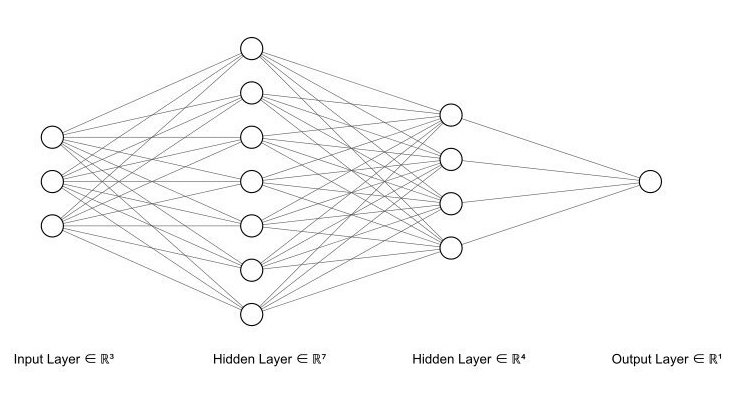
\includegraphics[width=\linewidth]{neural_net}
      \caption{A neural network with input $x\in \R^4$ and output $y\in\R^2$. The five hidden layers have dimensions $3$, $4$, $5$, $3$ and $7$ respectively. The graphic was generated with http://alexlenail.me/NN-SVG/index.html}\label{img_nn}
	\end{minipage}
\end{center}
\end{figure}


\section{Training of neural networks}\label{sec:training_of_nn}

Since we now know what neural networks are, we want to discuss how to tune them to a specific problem. This procedure is usually referred to as training of a neural network. There are many approaches of how to train a neural network. However, all of them require the definitions of a loss function and risk function. The loss function is a function that measures the point-wise error of a neural network, or any other prediction function in general. This is fundamental in supervised learning. In contrast, the risk function is a function that measures the error with regard to a probability measure or an observed data set.


\begin{definition}\label{def:loss}
Let $X,Y$ be arbitrary input and output spaces. Furthermore, let $t\in\R^n$ be a prediction for $y\in Y$.\\
Then we define a \textbf{supervised loss function} $\loss: X \times Y \times \R^n \to [0, \infty)$ as a measurable function that compares a true value $y \in Y \subset \R^n$ to a predicted value $\hat{y} = t$ in a suitable way.
\end{definition}

The recently introduced loss function from Definition \ref{def:loss} allows us to compare a true label to a prediction. However, since we only require it to be measurable, the function is defined very general. This is solely, because one may be interested in different loss functions in different settings, since the choice of a specific loss functions is a crucial aspect of learning theory, as it directly impacts the behaviour of learning algorithms.\\
We want to consider a couple of important examples for loss functions, for further reading please take a look at \cite[Chapter~4.3]{goodfellow2016deep}.


\begin{example}
Let $y\in Y\coloneqq \R$ and $t\in \R$, then the following functions are loss functions.
\begin{mydescription}{\widthof{\textbf{Squared Error Loss}}}
\item[\textbf{Squared Error Loss}] $\loss(y, t) = \left|y - t\right|^2$,
\item[\textbf{Linear Error Loss}]  $\loss(y, t) = \left|y - t\right|$.
\end{mydescription}
Now, let $y\in Y \coloneqq \R^n$ and $t\in\R^n$ with $n>1$. Then, we consider the squared error loss and the linear error loss pointwise:
\begin{mydescription}{\widthof{\textbf{Squared Error Loss}}}
\item[\textbf{Squared Error Loss}] $\loss(y, t) = \sum_{i=1}^n\left|y_i - t_i\right|^2$,
\item[\textbf{Linear Error Loss}]  $\loss(y, t) = \sum_{i=1}^n\left|y_i - t_i\right|$,
\end{mydescription}
where $y = (y_1,\ldots, y_n)$ and $t = (t_1,\ldots, t_n)$.
\end{example}


However, loss functions only quantify the disparity between one predicted outcome and one actual value. In order to compare the predictions over a wider range of data points, we need to introduce another quantity, the risk function.


\begin{definition}\label{def:risk}
Let $X,Y$ be arbitrary input and output spaces, $\loss$ be a supervised loss function and $\prob$ be a probability measure on $X \times Y$.\\
Then we define the \textbf{risk of the function $f$} with regard to a loss function $\loss$ as
\begin{align*}
\risk_{\loss, \prob}(f) = \int_{X\times Y} \loss\left(x, y, f(x) \right) d \prob(x, y).
\end{align*}
In the following, we will denote this as the \textbf{$\loss$-risk of $f$}.
\end{definition}


Considering applications, one usually wants to compute the risk with regard to observed data instead of a probability measure, since the true probability measure usually is unknown. In this case, the general risk function becomes more tangible, as we see in the following definition.


\begin{definition}\label{def:empirical_risk}
Let $X, Y$ be arbitrary input and output spaces, $D = \left((x_1,y_1), \ldots, (x_k,y_k)\right)$ be a dataset consisting of $k\in\N$ data points. Furthermore, let $\loss$ be a supervised loss function and $f$ be an arbitrary prediction function.\\
Then we define the \textbf{empirical risk function} as
\begin{align*}
\risk_{\loss, D} (f) = \frac{1}{k} \sum_{i=1}^{k} \loss\left(x_i, y_i, f(x_i)\right).
\end{align*}
We will write $\risk \coloneqq \risk_{\loss, D}$ unless unclear in the given context.
\end{definition}


With the previous definitions, we can return to considering the training of neural networks. There are many possible techniques and strategies. However, most of them rely on iteratively finding the gradient - the direction of greatest ascent of the risk function, and afterwards performing a step in the opposite of the found direction. This approach dates way back to the early $\nth{19}$ century and was introduced by Augustin L. Cauchy in the year $1847$. For a brief overview please take a look at \cite{lemarechal2012cauchy}. This method is immensely popular and thus, can be discovered in numerous literary works. We will mostly draw inspiration form \cite[Chapter~XV]{kantorovich2016functional}. For in-depth explanation, please take a look at the reference.\\
Let us consider a (non-linear) real-valued function $f$, which is defined on a real normed space $X$. We assume that $f$ is bounded below on $X$ and we aim to find an element $x^{\ast}\in X$ such that

\begin{align*}
f(x) \geq f(x^{\ast}),
\end{align*}

for all $x\in X$. Hence, $x^{\ast}$ minimizes the function $f$. To solve this problem, one usually constructs a sequence $(x_n)$ that minimizes $f$, in the sense that

\begin{align*}
\lim_{n\to\infty} f(x_n) = \inf_{x\in X} f(x).
\end{align*}

In certain cases, one can construct such a sequence that it converges to an optimum $x^{\ast}$. If the considered function $f$ is assumed to be continuous, then this element will be a solution to the proposed problem.\\
To construct such a sequence, we assume that the function $f$ is differentiable. This means, that the derivative

\begin{align*}
\frac{\partial f (x)}{\partial z} = \frac{1}{\|z\|} \lim_{h \to 0^+} \frac{f(x + hz) - f(x)}{h},
\end{align*}
exists at each point $x \in X$ and for every direction $z \in X$. We call such a function simply \textbf{differentiable}. If the function and its derivative are additionally continuous, we call it \textbf{continuously differentiable}.\\
Furthermore, we assume that there exists a direction for which the derivative takes minimum value - thus, the direction of steepest descent. This direction is essentially the negative direction of the gradient of $f$. If we now perform a step towards the direction of steepest descent, we completed an iteration of the so called steepest descent method - or nowadays better known as the gradient descent algorithm. This algorithm we now want to define a little more precisely.\\
Let $X$ be a normed space and $f:X\to \R$ be a continuously differentiable function with existing minimum $f(x^{\ast)}$.
Furthermore, let there be a direction of steepest descent in every $x \in X$ and $x^{(0)}\in X$ an arbitrary (initial) element. Assume that we already found the $k$-th iterate $x^{(k)}$, then we define the $(k+1)$-th iterate by

\begin{align}\label{eq:gd}
x^{(k+1)} = x^{(k)} - \g_{k+1} z_{k+1},
\end{align}

where $z_{k+1}$ denotes the direction of steepest descent at $x^{(k)}$. The numerical parameter $\g^{(k+1)}$ can be found in various ways. However, we propose the following one.\\
We specify a sequence of positive numbers $(\g_k)$ such that $\g_k \to 0$ and $\sum_{k\geq 1} \g_k = \infty$. Furthermore, we assume the $z_k$ to be normalized for all $k\in \N$, i.e. $\|z_k\| = 1$. Hence, the descent value at the $k$-th iteration is $\g_k$. We do this in order to avoid doing to great steps, which would eventually avert the convergence of the algorithm.\\
Furthermore, we note at this point that we can establish a connection between the problem of minimizing a functional and that of solving a linear functional equation as follows.\\
Let $U$ be a self-adjoint operator on a Hilbert space $\H$. We assume that the operator $U$ is below bounded by $m>0$ and above bounded by $M>0$. Now, lets consider the linear functional equation

\begin{align}\label{eq:lfe}
Ux = y,
\end{align}

since the inverse operator $U^{-1}$ exists (because the eigenvalue $\lambda = 0$ does not belong to the spectrum, see \cite[Theorem~IX.5.3]{kantorovich2016functional}), there exists one unique solution to \eqref{eq:lfe}, for each $y\in\H$. Now, we define the functional

\begin{align}\label{eq:functional}
F(x) = \left\langle Ux, x\right\rangle - \left( \left\langle x, y\right\rangle + \left\langle y, x\right\rangle \right).
\end{align}

With the help of the functional \eqref{eq:functional} we can formulate the following theorem.

\begin{theorem}\label{theorem:min_lfe}
Let $\H$ be a Hilbert space. A solution $x^{\ast}\in \H$ of \eqref{eq:lfe} yields a minimum of \eqref{eq:functional}. Conversely, if \eqref{eq:functional} attains a minimum at $x^{\prime} \in \H$, then $x^{\prime}$ is a solution of \eqref{eq:lfe}: that is: $x^{\prime} = x^{\ast}$.
\end{theorem}

\begin{proof}
Since we assumed $x^{\ast} \in \H$ to be a solution of \eqref{eq:lfe}, we can express $F$ as
\begin{align}\label{eq:F_rewritten}
F(x) = \left\langle Ux, x \right\rangle - \left\langle x, Ux^{\ast} \right\rangle - \left\langle Ux^{\ast}, x \right\rangle = \left\langle U(x - x^{\ast}), x - x^{\ast} \right\rangle - \left\langle Ux^{\ast}, x^{\ast} \right\rangle.
\end{align}
Using the boundedness of $U$ we receive
\begin{align}\label{eq:1.8}
F(x) \geq m\left\langle x - x^{\ast}, x - x^{\ast} \right\rangle - \left\langle Ux^{\ast}, x^{\ast} \right\rangle &\geq - \left\langle Ux^{\ast}, x^{\ast} \right\rangle\nonumber\\
&= \left\langle Ux^{\ast}, x^{\ast} \right\rangle  -2\left\langle Ux^{\ast}, x^{\ast} \right\rangle = F(x^{\ast}).
\end{align}
That is, $x^{\ast} \in \H$ indeed minimizes the functional $F$.\\
to prove the second part of the theorem, we will use the same inequality. Lets first consider the following equation and the definition of the functional \eqref{eq:functional}
\begin{align*}
0 = F(x^{\prime}) - F(x^{\ast}) &= \left\langle Ux^{\prime}, x^{\prime}\right\rangle - \left( \left\langle x^{\prime}, y\right\rangle + \left\langle y, x^{\prime}\right\rangle \right)- \left\langle Ux^{\ast}, x^{\ast}\right\rangle - \left( \left\langle x^{\ast}, y\right\rangle + \left\langle y, x^{\ast}\right\rangle \right)\\
&=\left\langle Ux^{\prime}, x^{\prime}\right\rangle - \left( \left\langle x^{\prime}, y\right\rangle + \left\langle y, x^{\prime}\right\rangle \right)
+ \left\langle Ux^{\ast}, x^{\ast}\right\rangle,
\end{align*}
where in the last step we used the same equation as on the right-hand side of \eqref{eq:1.8}.\\
Now we use the fact, that $x^{\ast}$ solves the equation \eqref{eq:lfe}.
\begin{align*}
\left\langle Ux^{\prime}, x^{\prime}\right\rangle - \left( \left\langle x^{\prime}, y\right\rangle + \left\langle y, x^{\prime}\right\rangle \right)
+ \left\langle Ux^{\ast}, x^{\ast}\right\rangle
&= \left\langle Ux^{\prime}, x^{\prime}\right\rangle - \left( \left\langle x^{\prime}, Ux^{\ast}\right\rangle + \left\langle Ux^{\ast}, x^{\prime}\right\rangle \right) + \left\langle Ux^{\ast}, x^{\ast}\right\rangle.
\end{align*}
The next step is to use the fact that $U$ is a self-adjoint operator.
\begin{align*}
&\left\langle Ux^{\prime}, x^{\prime}\right\rangle - \left( \left\langle x^{\prime}, Ux^{\ast}\right\rangle + \left\langle Ux^{\ast}, x^{\prime}\right\rangle \right)
+ \left\langle Ux^{\ast}, x^{\ast}\right\rangle\\
&\qquad= \left\langle Ux^{\prime}, x^{\prime}\right\rangle - \left( \left\langle Ux^{\prime}, x^{\ast}\right\rangle + \left\langle Ux^{\ast}, x^{\prime}\right\rangle \right)	+ \left\langle Ux^{\ast}, x^{\ast}\right\rangle.
\end{align*}
Lastly, we use the linearity of the inner product and the lower bound of the operator $U$.
\begin{align*}
\left\langle Ux^{\prime}, x^{\prime}\right\rangle - \left( \left\langle Ux^{\prime}, x^{\ast}\right\rangle + \left\langle Ux^{\ast}, x^{\prime}\right\rangle \right)
+ \left\langle Ux^{\ast}, x^{\ast}\right\rangle &=\left\langle U(x^{\prime} - x^{\ast}), x^{\prime} - x^{\ast} \right\rangle\\
&\geq m \left\langle x^{\prime} - x^{\ast}, x^{\prime} - x^{\ast} \right\rangle,
\end{align*}
therefore, $x^{\prime} = x^{\ast}$.
\end{proof}

Furthermore, we realise that the application of the gradient descent algorithm to the functional \eqref{eq:functional} leads to a sequence that converges to $x^{\ast}$, which is a solution to \eqref{eq:lfe} as we saw in Theorem \ref{theorem:min_lfe}. Now, lets take a look at how applying the gradient descent algorithm to the functional $F$ would look like, in particular.

\begin{corollary}\label{cor:gd}
Let $\H$ be a Hilbert space and $F$ be a functional as defined in \eqref{eq:functional}.\\
Then the gradient descent algorithm applied to the functional $F$ with arbitrary initial iterate $x^{(0)}\in\H$ looks like
\begin{align*}
x^{(k)} = x^{(k-1)} - \g_{k-1}z_{k-1},
\end{align*}
where $z_k\in\H$ and $\g_k>0$ look like
\begin{align*}
z_k = Ux^{(k-1)} - y \qquad\text{and} \qquad\g_k = \frac{\langle z_k, z_k \rangle}{\langle Uz_k, z_k \rangle}.
\end{align*}
\end{corollary}

\begin{proof}
Let $x, z\in \H$, then
\begin{align}\label{eq:F_dir}
F(x + z) &= \left\langle U(x + z), x + z \right\rangle - \left( \left\langle x + z, y \right\rangle + \left\langle y, x + z \right\rangle  \right)\nonumber\\
&= \left\langle Ux, x \right\rangle - \left( \left\langle x, y \right\rangle + \left\langle y, x \right\rangle  \right) + \left( \left\langle Ux - y, z \right\rangle + \left\langle z, Ux - y \right\rangle \right) + \left\langle Uz, z \right\rangle\nonumber\\
&= F(x) + \left( \left\langle Ux - y, z \right\rangle + \left\langle z, Ux - y \right\rangle \right) + \left\langle Uz, z \right\rangle.
\end{align}
Considering the derivative in direction $z$ gives us
\begin{align*}
\frac{\partial F}{\partial z} (x) = \frac{1}{\|z\|} \left(  \left\langle Ux - y, z \right\rangle + \left\langle z, Ux - y \right\rangle \right) = \frac{2 \langle Ux - y, z \rangle}{\|z\|},
\end{align*}
where in the last equation we used the fact that $F$ is a real-values function.\\
Thus the direction of steepest ascent at $x^{(0)}\in\H$ is given by $z_1 = Ux^{(0)} - y$ and the direction of steepest descent by $-z_1$.\\
Lastly, to determine the descent value we consider the equation \textcolor{red}{The author considered rays, i.e. $\phi(\a;x, z) = \Phi(x+\a z)$, I guess we need to do the same?}
\begin{align*}
\lim_{h\to 0^+} \frac{F(x^{(0)} - hz_1) - F(x^{(0)})}{h} = 0,
\end{align*}
where with the use of equation \eqref{eq:F_dir}, we have
\begin{align*}
F(x^{(0)} - z_1) = F(x^{(0)}) - 2 \left\langle z_1, z_1 \right\rangle + \left\langle Uz_1, z_1 \right\rangle,
\end{align*}
what ultimately leads to the step size
\begin{align*}
\g_1 = \frac{\langle z_1, z_1 \rangle}{\langle Uz_1, z_1 \rangle}.
\end{align*}
In exactly the same way, $\g_k$ and $z_k$ can be determined for all $k>1$ and hence, all assertions from the theorem are proven.
\end{proof}

The gradient descent algorithm with parameters as asserted in Corollary \ref{cor:gd} does converge, as we have seen in the proof. However, one might pose the question how quickly it converges. This question we want to consider in the following theorem.

\begin{theorem}
Let the same assumptions as in Corollary \ref{cor:gd} hold. Then the constructed sequence $(x^{(n)})$ with $(z_k), (\g_k)$ as in Corollary \ref{cor:gd}, converges to $x^{\ast}\in\H$. Its speed of convergence is given by
\begin{align*}
\left\|x^{(n)} - x^{\ast}\right\| \leq \frac{\|z_1\|}{m}\left( \frac{M - m}{M + m} \right)^n,
\end{align*}
for all $n\in\N_0$.
\end{theorem}

\begin{proof}
Firstly, we rewrite the equation \eqref{eq:lfe} to
\begin{align}\label{eq:rewritten}
Ux &= y\nonumber\\
\Longleftrightarrow \qquad 0 &= ky - kUx\nonumber\\
\Longleftrightarrow \qquad x &= x - kUx + ky.
\end{align}
We chose the numerical factor $k>0$ in a way, that the operator $T=I-kU$ has the smallest possible norm. Since we assumed $U$ to be lower bounded by $m$ and upper bounded by $M$, the operator $T$ needs to be lower bounded by $1-km$ and upper bounded by $1-kM$, where the minimal norm will occur if
\begin{align*}
1-km = -(1-kM).
\end{align*}
This leads to
\begin{align*}
k = \frac{2}{m + M}.
\end{align*}
Therefore, for $\|T\|$ holds
\begin{align}\label{eq:lower}
\|T\| = 1 - km = 1 - \frac{2m}{m+M},
\end{align}
as well as
\begin{align}\label{eq:upper}
\|T\| = kM - 1 = \frac{2M}{m+M} - 1.
\end{align}
Combining the equations \eqref{eq:lower} and \eqref{eq:upper} leads to
\begin{align*}
2\|T\| &= \left( 1 - \frac{2m}{m+M}\right) + \left( \frac{2M}{m+M} - 1\right) = \frac{2M - 2m}{m+M}\\
\Longleftrightarrow \qquad \|T\| &= \frac{M-m}{M+m}.
\end{align*}
Moreover, applying \eqref{eq:rewritten} and rewriting it gives us
\begin{align}\label{eq:x_prime}
x^{\prime}_1 = Tx^{(0)} + ky = x^{(0)} - k(Ux^{(0)} - y) = x^{(0)} - kz_1.
\end{align}
Let us introduce the operator $V = U^{1/2}$ and plug it into \eqref{eq:F_rewritten}. Note that since $U$ is a self-adjoint operator, so is $V$ (see \cite[Theorem~V.6.2]{kantorovich2016functional}).
\begin{align}\label{eq:F_rewritten2}
F(x) &= \left\langle U(x - x^{\ast}), x - x^{\ast} \right\rangle - \left\langle Ux^{\ast}, x^{\ast} \right\rangle\nonumber\\
&= \left\langle V(x - x^{\ast}), V(x - x^{\ast}) \right\rangle - \left\langle Vx^{\ast}, Vx^{\ast} \right\rangle\nonumber\\
&= \left\|V(x - x^{\ast}) \right\|^2 - \left\|Vx^{\ast} \right\|^2
\end{align}
Considering the inequality $F(x^{\prime}_1) \geq F(x^{(1)})$, which holds due to the fact that $x^{(1)}$ is the iterate performed with optimal descent value (\textcolor{red}{at least the author proposes? Feels somewhat awkward though}), leads to
\begin{align*}
F(x^{(1)}) -F(x^{\ast}) \leq F(x^{\prime}_1) -F(x^{\ast}),
\end{align*}
which we can rewrite again with the use of \eqref{eq:F_rewritten2}
\begin{align}\label{ineq:1}
\left\| V(x^{(1)} - x^{\ast}) \right\| \leq \left\| V(x^{\prime}_1 - x^{\ast}) \right\|.
\end{align}
Since equation \eqref{eq:F_rewritten} was the rewritten equation \eqref{eq:lfe}, we can write with the definition of $T$
\begin{align*}
x^{\ast} = Tx^{\ast} + ky,
\end{align*}
subtracting this equation from \eqref{eq:x_prime} gives us
\begin{align*}
x^{\prime}_1 - x^{\ast} = T(x^{(0)} - x^{\ast}),
\end{align*}
applying the operator $V$ on both sides gives us
\begin{align}\label{eq:1.16}
V\left(x^{\prime}_1 - x^{\ast}\right) = VT(x^{(0)} - x^{\ast}).
\end{align}
With the easy calculation
\begin{align*}
VT = V\left( I - kU\right) = V -kVU = V - kVVV = \left(I-kU\right)V = TV,
\end{align*}
we realise that the operators $T$ and $V$ commute. Hence, we can rewrite \eqref{eq:1.16} to
\begin{align*}
V\left(x^{\prime}_1 - x^{\ast}\right) = TV(x^{(0)} - x^{\ast}).
\end{align*}
Considering the norm leads to
\begin{align*}
\left\|V\left(x^{\prime}_1 - x^{\ast}\right)\right\| &= \left\| TV(x^{(0)} - x^{\ast})\right\| \leq \left\| T \right\| \left\|V(x^{(0)} - x^{\ast})\right\|\\
&=\frac{M-m}{M+m} \left\|V(x^{(0)} - x^{\ast})\right\|\\
\end{align*}
Therefore, with inequality \eqref{ineq:1} we have
\begin{align*}
\left\| V(x^{(1)} - x^{\ast}) \right\|\leq \frac{M-m}{M+m} \left\|V(x^{(0)} - x^{\ast})\right\|.
\end{align*}
If we apply exactly the same arguments for all $k\in\{1,\ldots n\}$, then we have the following bound for the $n$-th iterate
\begin{align*}
\left\| V(x^{(n)} - x^{\ast}) \right\|\leq \frac{M-m}{M+m} \left\|V(x^{(n-1)} - x^{\ast})\right\|,
\end{align*}
which leads to the bound
\begin{align*}
\left\| V(x^{(n)} - x^{\ast}) \right\|\leq \left(\frac{M-m}{M+m}\right)^n \left\|V(x^{(0)} - x^{\ast})\right\|.
\end{align*}
Furthermore, we realise that the function $t^{-1/2}$ is continuous in $[m, M]$ and therefore especially on the spectrum of $U$, which leads to the observation that the inverse operator $V^{-1/2}$ exists.\\
Moreover, with the help of \cite[Theorem~V.6.2]{kantorovich2016functional} (which regards the spectrum $S_U$ of the operator $U$) the following equations hold
\begin{align*}
\left\|V^{-1}\right\| &= \max_{t\in S_U} \frac{1}{\sqrt{t}} = \frac{1}{\sqrt{m}},\\
\left\|V\right\| &= \max_{t\in S_U} \sqrt{t} = \sqrt{M}.
\end{align*}
Combining the above results, we receive
\begin{align}\label{eq:combined}
\left\| x^{(n)} - x^{\ast} \right\| = \left\| V^{-1}V\left(x^{(n)} - x^{\ast}\right) \right\|&\leq \left\| V^{-1}\right\| \left\|V\left(x^{(n)} - x^{\ast}\right) \right\|\nonumber\\
&\leq \left\| V^{-1}\right\|\left( \frac{M-m}{M+m} \right)^n \left\|V\left(x^{(0)} - x^{\ast}\right) \right\|\nonumber\\
&\leq \frac{1}{\sqrt{m}}\left( \frac{M-m}{M+m} \right)^n \left\|V\left(x^{(0)} - x^{\ast}\right) \right\|.
\end{align}
However, since the unknown element $x^{\ast}$ appears on the right-hand side, we want to somehow remove it. In order to do this, we consider
\begin{align*}
\left\|V(x^{(0)} - x^{\ast}) \right\| = \left\|V^{-1}U(x^{(0)} - x^{\ast}) \right\| \leq \left\|V^{-1}\right\| \left\|U(x^{(0)} - x^{\ast}) \right\| = \frac{\|z_1\|}{\sqrt{m}}.
\end{align*}
Plugging this result into \eqref{eq:combined}, gives us
\begin{align*}
\left\| x^{(n)} - x^{\ast} \right\| \leq \frac{\|z_1\|}{m}\left( \frac{M-m}{M+m} \right)^n.
\end{align*}
This is exactly the inequality asserted in the theorem.
\end{proof}

\textcolor{red}{TODO: Here we should show how to compute the gradient of a risk, where a neural network is considered as a prediction function. This would show that in applications it is very expensive to compute the gradient with regard to the whole dataset, which is the motivation for SGD.}

However, the gradient descent algorithm relies on computing the gradient of the risk function in each iteration, which oftentimes is too expensive and therefore is being relaxed by only considering the gradient in one sample (or multiple samples, we speak of a mini-batch then). We want to take a closer look at this algorithm as well. Since it is quite popular, there are many good references in literature, e.g see \cite[Chapter~13.3.2]{sra2012optimization}, \cite[Chapter~4.2]{saad2009line} and \cite{turinici2021convergence}. We will focus on the latter reference.\\
Beforehand, we need to consider the empirical risk, which we defined in Definition \ref{def:empirical_risk}. Since we take the average of the loss functions with regard to the whole data set $D$, we can denote it as an integral over the dataset $D$
\begin{align*}
\risk_{\loss, D} (f) = \frac{1}{k} \sum_{i=1}^{k} \loss\left(x_i, y_i, f(x_i)\right) = \int_{D} \loss(x,y,f(x)) d(x,y).
\end{align*}
If we now randomly choose a subset $B \subseteq D$ of length $b\in\{1,\ldots,n\}$ which we will call \textbf{mini-batch of size $b$}, we can approximate the empirical risk $\risk_{\loss, D} (f)$ through $\risk_{\loss, B} (f)$.
\begin{align*}
\risk_{\loss,B}(f) = \int_{B}\loss(x, y, f(x)) d(x,y).
\end{align*}
One may quickly realise, that if $b=n$, we are in the regular gradient descent setting. If one chooses to be $b=1$, i.e. the subset $B$ consisting of one single sample, then we speak of \textbf{stochastic gradient descent}, otherwise of \textbf{stochastic gradient descent with batch-size $b$}.\\
In the following, we want to summarize the data samples $\o_i=(x_i,y_i)$. Hence, we can write
\begin{align*}
\risk_{\loss,B}(f) = \int_{B}\loss(\o, f(x)) d\o.
\end{align*}
Furthermore, we remember that we essentially are interested in the setting, where $f$ is a neural network. Since the neural network $f$ has parameters $\t$, which we denoted as $f_{\t}$, we will now simply the notation as follows
\begin{align*}
\risk_{\loss,B}(f_{\t}) = \int_{B}\loss(\o, f_{\t}(x)) d\o \eqqcolon \int_{B}\loss(\o,\t) d\o \eqqcolon \risk_{\loss,B}(\t).
\end{align*}
Our goal is to find a minimum of $\risk_{\loss,B}$, we approach this problem the same way as we approached the gradient descent algorithm, where we iteratively update the parameters $\t$ to minimize the risk. Therefore, we define the update rule as follows. Lets assume we already found the $k$-th iterate $\t^{(k)}$. Now we randomly choose a sample $\o_k$ and compute its loss with regard to the current parameters $\t^{(k)}$. Afterwards, we compute the gradient of the empirical risk in the sample $\o_k$ and update the parameters. This looks like
\begin{align}\label{eq:sgd}
\t^{(k+1)} = \t^{(k)} -\g_k \nabla_{\t} \loss(\o_k,\t^{(k)}).
\end{align}
This way we define a sequence of parameters $(\t^{(k)})$, which we will show to converge to some $\t^{\ast}$ that minimizes the empirical risk $\risk_{\loss,B}(\t)$.
However, to prove this convergence we need to pose some assumptions.
\begin{assumption}\label{ass:sgd}
We assume that the risk function $\risk_{\loss,\o}$ meets the following conditions.
\begin{enumerate}
\item The gradient of $\risk_{\loss,\o}(\t)$ is bounded, i.e.
\begin{align}\label{eq:ass1}
\exists G > 0: \sup_{\o\in D} \left\| \nabla_{\t} \risk_{\loss,\o}(\t) \right\|^2 \leq G,
\end{align}
for all $\t\in\T$.
\item $\risk_{\loss,\o}(\t)$ is strongly convex, i.e.
\begin{align}\label{eq:ass2}
\exists \m>0: \risk_{\loss,\o}(\t_2) \geq \risk_{\loss,\o}(\t_1) + \left\langle \nabla_{\t} \risk_{\loss,\o}(\t_2), \t_2-\t_1 \right\rangle + \frac{\m}{2} \left\| \t_1 - \t_2 \right\|^2,
\end{align}
for all $\t_1,\t_2 \in\T$.
\end{enumerate}
\end{assumption}
At this point we should note that the second assumption is quite restrictive and can indeed be relaxed. Since neural networks rarely are convex and especially not strictly convex functions, the corresponding empirical risk function is neither. However, relaxing this assumption makes the proof far more challenging, what we do not want to tackle in this thesis. Instead we want to reference e.g. \cite{lei2019stochastic}, where the authors prove the stochastic gradient descent algorithm to converge even for non-convex functions, which still have to fulfil some constraints, such as Hölder continuity and the Polyak-\L{}ojasiewicz condition. Nonetheless, these conditions are far less restrictive and neural networks are proposed to meet those.\\
Having explored nuances of the made assumptions, we now return to the central focus, which is the convergence of the stochastic gradient descent algorithm.

\begin{theorem}\label{theorem:sgd}
Let $(\O, \A, \prob)$ be a probability space, $X$, $Y$ be arbitrary input and output spaces and $\T$ an arbitrary parameter space. Furthermore, let $\loss$ denote an arbitrary supervised loss function and let the corresponding empirical risk $\risk_{\loss, \o}$ be continuously differentiable in every $\o\in X\times Y$.\\
Then the stochastic gradient descent algorithm with update rule \eqref{eq:sgd} and posed Assumption \ref{ass:sgd} satisfies the following assertions.
\begin{enumerate}
\item \label{ass1} The empirical risk function $\risk_{\loss, \o}$ has a unique minimum at $\t^{\ast}\in\T$.
\item \label{ass2}For any $n\geq 0$ denote $d_n$ as
\begin{align}\label{eq:dist}
d_n = \E \left( \left\| \t^{(n)} - \t^{\ast} \right\|^2 \right).
\end{align}
Then for $d_{n+1}$ holds
\begin{align}\label{eq:dist_rec}
d_{n+1} \leq (1 - \g_n\m)d_n + \g_n^2B.
\end{align}
\item \label{ass3}For any $\e>0$ there exists a $\g>0$ such that if $\g_n=\g$, then
\begin{align}\label{eq:limsup}
\limsup_{n\to \infty} \left( \left\| \t^{(n)} - \t^{\ast} \right\|^2 \right) \leq \e.
\end{align}
\item \label{ass4} If the sequence $(\g_n)$ meets the conditions
\begin{align}\label{eq:step_size}
\g_n\to 0 \qquad \text{and} \qquad \sum_{n\geq 0} \g_n = \infty,
\end{align}
then $d_n\to 0$, that is $\lim_{n\to\infty}\t^{(n)} = \t^{\ast}$, where the convergence is the $L^2$-convergence of random variables, see e.g. \cite[Chapter~7]{klenke2013probability}.
\end{enumerate}
\end{theorem}

\begin{proof}
\textit{Assertion~\ref{ass1}}: The existence of a minimum follows from the continuity and lower boundedness of $\risk_{\loss, \o}$. The uniqueness follows from the strong convexity of $\risk_{\loss, \o}$.\\
\textit{Assertion~\ref{ass2}}: It holds that
\begin{align}\label{eq:item2}
&d_{n+1} = \E\left( \left\| \t^{(n+1)} - \t^{\ast} \right\|^2 \right) = \E\left( \left\| \t^{(n)} - \t^{\ast} - \g_n \nabla_{\t} \loss(\o_n, \t^{(n)}) \right\|^2 \right)\nonumber\\
&\quad= \E\left( \left\| \t^{(n)} - \t^{\ast}\right\|^2 \right) - 2\g_n\E\left(\left\langle \t^{(n)}- \t^{\ast}, \nabla_{\t}\loss(\o_n, \t^{(n)}) \right\rangle\right) + \E \left( \g_n^2 \left\| \nabla_{\t} \loss(\o_n, \t^{(n)}) \right\|^2 \right).
\end{align}
First, we consider that
\begin{align*}
\E\left( \left\langle \t^{(n)} - \t^{\ast}, \nabla_{\t}\loss(\o_n, \t^{(n)}) \right\rangle \right)= \E\left( \t^{(n)} - \t^{\ast}, \nabla_{\t} \risk_{\loss, \o_n} \right),
\end{align*}
what we can bound with the help of the second assumption \eqref{eq:ass2} by
\begin{align*}
\E\left( \t^{(n)} - \t^{\ast}, \nabla_{\t} \risk_{\loss, \o_n} \right) \geq
\E\left( \risk_{\loss, \o_n} (\t^{(n)})	 - \risk_{\loss, \o_n} (\t^{\ast}) + \frac{\m}{2} \left\| \t^{(n)} - \t^{\ast} \right\|^2	\right).
\end{align*}
Since $\t^{\ast}$ minimizes $\risk_{\loss, \o}$, the difference $\E(\risk_{\loss, \o_n} (\t^{(n)})) - \E(\risk_{\loss, \o_n} (\t^{\ast}))$ is positive and we can bound this even further to
\begin{align*}
\E\left( \risk_{\loss, \o_n} (\t^{(n)})	 - \risk_{\loss, \o_n} (\t^{\ast}) + \frac{\m}{2} \left\| \t^{(n)} - \t^{\ast} \right\|^2	\right) \geq
\frac{\m}{2}\E\left( \left\| \t^{(n)} - \t^{\ast} \right\|^2\right).
\end{align*}
Lastly, we consider \eqref{eq:item2} and use the first assumption \eqref{eq:ass1}. This gives us
\begin{align*}
&\E\left( \left\| \t^{(n)} - \t^{\ast}\right\|^2 \right) - 2\g_n\E\left(\left\langle \t^{(n)}- \t^{\ast}, \nabla_{\t}\loss(\o_n, \t^{(n)}) \right\rangle\right) + \E \left( \left\| \nabla_{\t} \loss(\o_n, \t^{(n)}) \right\|^2 \right)\\
&\quad\leq d_n - \g_n\m d_n + \g_n^2B = \left(1 - \g_n\m\right)d_n + \g_n^2B.
\end{align*}
\textit{Assertion~\ref{ass3}}: Assume that $(\g_n)$ is a constant sequence with value $\g>0$. Then the inequality \eqref{eq:dist_rec} is equal to
\begin{align}\label{ineq:2}
d_{n+1} &\leq (1 - \g\m)d_n + \g^2B\nonumber\\
\Longleftrightarrow \qquad d_{n+1} - \g\frac{B}{\m} &= \left(1 - \g\m\right)d_n + \g^2\frac{\m}{\m} B - \g\frac{B}{\m}\nonumber\\
\Longleftrightarrow \qquad d_{n+1} - \g\frac{B}{\m} &= \left(1 - \g\m\right)\left(d_n - \g\frac{B}{\m}\right).
\end{align}
Furthermore, one may quickly realise that by applying inequality \eqref{ineq:2} twice holds
\begin{align*}
d_{n+2} - \g\frac{B}{\m} \leq \left(1 - \g\m\right)\left(1 - \g\m\right)\left(d_{n+1} - \g\frac{B}{\m}\right) \leq \left(1 - \g\m\right)^2\left(d_n - \g\frac{B}{\m}\right).
\end{align*}
Therefore, by applying inequality \eqref{ineq:2} $k$ times we receive
\begin{align*}
d_{n+k} - \g\frac{B}{\m} \leq \left(1 - \g\m\right)^k\left(d_n - \g\frac{B}{\m}\right).
\end{align*}
Since $d_n>0$ for all $n\geq 0$ by construction, taking $k\to\infty$ we obtain
\begin{align*}
\limsup_{k\to\infty} \left( d_{k} - \g\frac{B}{\m} \right) = 0,
\end{align*}
or equally
\begin{align*}
\limsup_{k\to\infty} \left( d_{k}\right) = \g\frac{B}{\m}.
\end{align*}
Lastly, since we are free to choose the constant $\g$, we define it as $\g\coloneqq \e \m/B$. This gives us
\begin{align*}
\limsup_{k\to\infty} \left( d_{k}\right) = \limsup_{k\to \infty} \left( \left\| \t^{(k)} - \t^{\ast} \right\|^2 \right) \leq \e.
\end{align*}
\textit{Assertion~\ref{ass4}}: Assume that the sequence $(\g_n)$ is non-constant and assume that $\e>0$. Furthermore, with the same idea as in inequality \eqref{ineq:2} we receive
\begin{align*}
d_{n+1} - \g_n\frac{B}{\m} \leq \left(1 - \g_n\m\right)\left(d_n - \g_n\frac{B}{\m}\right).
\end{align*}
If we now define $\e_n \coloneqq \g_nB/\m$, this gives us
\begin{align}\label{ineq:3}
d_{n+1} - \e_n \leq \left(1 - \g_n\m\right)\left(d_n - \e_n\right).
\end{align}
Therefore, applying inequality \eqref{ineq:3} twice gives us
\begin{align*}
d_{n+2} - \e_n \leq \left(1 - \g_n\m\right)\left(d_{n+1} - \e_n\right) \leq \left(1 - \g_{n+1}\m\right)\left(1 - \g_n\m\right)\left(d_n - \e_n\right).
\end{align*}
Applying inequality \eqref{ineq:3} $k$ times iteratively leads to
\begin{align}\label{ineq:iter}
d_{n+k} - \e_n \leq \prod_{l=n}^{n+k-1}\left(1 - \g_l\m\right)\left(d_n - \e_n\right).
\end{align}
Now, we consider the product on the right-hand side to fulfil
\begin{align*}
0 \leq \prod_{l=n}^{n+k-1}\left(1 - \g_l\m\right) = \exp \left(\sum_{l=n}^{n+k-1}\log\left(1 - \g_l\m\right) \right).
\end{align*}
since for $x\in (0,1)$ holds $\log(1-x) \leq -x$, we have
\begin{align*}
\exp \left(\sum_{l=n}^{n+k-1}\log\left(1 - \g_l\m\right) \right) \leq \exp \left(\sum_{l=n}^{n+k-1}\left(- \g_l\m\right) \right)\overset{k\to\infty}{\longrightarrow} \exp(-\infty) = 0,
\end{align*}
due to the assumption, that $\sum_{n\geq 0}\g_n = \infty$ and therefore, $\sum_{n\geq l}\g_n = \infty$  for $l\in\N$ as well.\\
Plugging this result into inequality \eqref{ineq:iter}, we receive
\begin{align*}
\lim_{k\to\infty}d_{n+k} - \e_n 0.
\end{align*}
Lastly, we note that $\e_n$ was defined as $\e_n = \g_n B/\m$, where $B, m$ are constants. Thus, since $\g_n$ is assumed to converge towards $0$, the same holds for $\e_n$. Therefore, it holds that
\begin{align*}
\lim_{n\to\infty}d_{n} = 0,
\end{align*}
which is exactly Assertion~\ref{ass4}.
\end{proof}

\iffalse
\textcolor{red}{TODO: THE WHOLE GD AND SGD THEORY WILL BE REWORKED!!! I consider introducing the gd and sgd algorithms as in \cite{DBLP:journals/corr/abs-1902-00908}. It will require some additional quantities (RKHS, Polyak-\L{}ojasiewiecz condition), but this PL-condition is satisfied by e.g. neural networks, what makes this highly interesting.}

\begin{theorem}\label{theorem_gd}
Let $(\g_t)_{t \in \N}$ be a sequence with $\g_t \to 0$. Furthermore, let $f:\R^n \to \R$ be a continuous, convex and differentiable function. Furthermore, let $x^{(t)}$ denote the $t$-th iterate of the \textbf{gradient descent algorithm} defined by
\begin{align}
x^{(t+1)} = x^{(t)} - \g_t \partial_x f(x^{(t)}),
\end{align}
with a suitable initial guess $x^{(0)}\in \R^n$.\\
Then the algorithm converges to the global minimum $f(x^{\ast})\in \R$, meaning
\begin{align*}
x^{\ast} \coloneqq \argmin_{x\in\R^n}f(x) = \lim_{t\to\infty} x^{(t)}.
\end{align*}
Lastly, if the function $f$ is strictly convex, then the global minimum $f(x^{\ast}) \in\R$ is unique.
\end{theorem}


\begin{proof}
If the step size is sufficiently small such that the iterate is contained in the sphere around $x^{\ast}$ with radius $d\left(x^{\ast}, x^{(t)}\right)$,
the iterate $x^{(t+1)}$ is bound by a sphere around $x^{\ast}$ with radius $d\left(x^{\ast}, x^{(t)} - \g_t \nabla_x f(x^{(t)})\right) < d\left(x^{\ast}, x^{(t)}\right)$, since
\begin{align*}
d\left(x^{\ast}, x^{(t)}\right) &\geq d\left(x^{\ast}, x^{(t+1)}\right)\\
&= d\left(x^{\ast}, x^{(t)} - \g_t \nabla_x f(x^{(t)})\right).
\end{align*}
Hence, the distance $d(x^{\ast}, x^{(t)})$ becomes smaller in each iteration, due to the convexity of $f$, with
\begin{align*}
\lim_{t\to\infty} d\left(x^{\ast}, x^{(t)}\right) = 0,
\end{align*}
since we know that $\R^n$ is a Banach space and $\left(d\left(x^{\ast}, x^{(t)}\right)\right)_{t\in\N}$ is a converging sequence by construction.\\
It is left to show, that if the function $f$ is strictly convex, then the global minimum $f(x^{\ast})\in\R$ is unique. This assertion holds, since if there were two global minima $f\left(x_1^{\ast}\right), f\left(x_2^{\ast}\right)$ with $x_1^{\ast} \neq x_2^{\ast}$.\\
Now consider $x^{\prime} \coloneqq \frac{x_1^{\ast} + x_2^{\ast}}{2}$, a point between $x_1^{\ast}$ and $x_1^{\ast}$. Since $f$ is assumed to be strictly convex, this leads to
\begin{align*}
f\left(x^{\prime} \right) = f\left(\frac{1}{2}x_1^{\ast} + \frac{1}{2} x_2^{\ast}\right) < \frac{1}{2} f\left(x_1^{\ast} \right) + \frac{1}{2} f\left(x_2^{\ast}\right) = f\left(x_1^{\ast}\right) = f\left(x_2^{\ast}\right).
\end{align*}
This would contradict the assumption that $f\left(x_1^{\ast}\right), f\left(x_2^{\ast}\right)$ are minima, especially global minima. Hence, the assertion holds.
\end{proof}


However, in order to apply the gradient descent algorithm to train neural networks, we have to consider how to actually compute the gradient of the empirical risk function, where we consider a neural network as prediction function.


\begin{lemma}\label{lemma:nn_gradient}
Let $f_\t:\R^d\to \R$ be a neural network with parameters $\t\in\T$, arbitrary depth $L_n\in\N$ and arbitrary activation function $\f$. Furthermore, let $D$ be a dataset of length $k\in \N$ and $L$ be an arbitrary loss function.\\
The gradient of the risk function $\risk(\cdot)$ with regard to the neural network $f_\t$ and thus the parameters $\t$ look as follows
\begin{align*}
\partial_\t \risk \left(f_{\t}\right) = \frac{1}{k} \sum_{i=1}^{k} \partial_\t L\left(x_i, y_i, f_\t(x_i)\right).
\end{align*}
Hence, it is the average of gradients in all data points $(x_i,y_i) \in D$.
\end{lemma}


\begin{proof}
To prove the assertion we simply use the Definition \ref{def:empirical_risk} of the empirical risk function and consider the linearity property of derivatives.
\begin{align*}
\partial_\t \risk \left(f_{\t}\right) &= \partial_\t \frac{1}{k} \sum_{i=1}^{k} L\left(x_i, y_i, f_\t(x_i)\right)\\
&= \frac{1}{k} \sum_{i=1}^{k} \partial_\t L\left(x_i, y_i, f_\t(x_i)\right).
\end{align*}
\end{proof}


With the previous definitions and results we can formulate the gradient descent algorithm for a neural network.


\begin{corollary}
Let $f_\t:\R^d\to \R$ be a neural network with parameters $\t\in\T$, arbitrary depth $L\in\N$ and arbitrary activation function $\f$. Let $(\g_t)_{t \in \N}$ be a sequence with $\g_t \to 0$ and $D$ be a dataset of length $k\in \N$.\\
Then one can train the neural network $f_\t$ with the gradient descent algorithm proposed in \eqref{eq:gd}. In this setting, the algorithm looks as follows
\begin{align*}
\t^{(t)} = \t^{(t - 1)} - \g_{t-1} \partial_\t \risk \left(f_{\t^{(t -1)}}\right),
\end{align*}
where the gradient can be computed as in Lemma \ref{lemma:nn_gradient}
\end{corollary}


\textcolor{red}{TODO:} Name some properties (convergence, rate, etc.) and reference them


This is a valuable result, since this way one can iteratively optimize any convex function. Such iterative methods are powerful in numerical settings, where one could use a machine to compute the result. However, there is one problem: in many practical cases it is way to expensive to compute the gradient with regard to the whole dataset, if the dataset becomes significantly large. This lead to a bunch of approaches on how to make this algorithm more efficient, one of those being the stochastic gradient descent algorithm.

\begin{theorem}\label{theorem:sgd}
Let $f_\t:\R^d\to \R$ be a neural network with parameters $\t\in\T$, arbitrary depth $L\in\N$ and arbitrary activation function $\f$. Let $(\g_t)_{t \in \N}$ be a sequence with $\g_t \to 0$ and $D$ be a dataset of length $k\in \N$.\\
Then we define the $t$-th iterate of the \textbf{stochastic gradient descent algorithm} by
\begin{align}
\t^{(t)} = \t^{(t - 1)} - \g_{t-1} \partial_{\t, i} \risk \left(f_{\t^{(t - 1)}}\right),
\end{align}
with $i \in \{1,\ldots, k\}$ and $\partial_{\t, i} \risk \left(f_{\t^{(t)}}\right)$ denoting the gradient with regard to the $i$-th data tuple $(x_i, y_i) \in D$.
\end{theorem}


\textcolor{red}{TODO:} Name some properties (convergence, rate, etc.) and reference them
\fi

Lastly, we want to consider another powerful optimization algorithm that adapts learning rates based on past gradient magnitudes and momenta - it is called \glqq Adaptive Moment Estimation (Adam)\grqq{}.\\
However, in order to formulate the algorithm formally we need to introduce stochastic moments first. We do so analogously to \cite[Chapter~5]{papoulis02}

\begin{definition}\label{def:moment}
Let $(\O,\A,\prob)$ be a probability space, $X$ be a random variable over $\O$ and $k\in\N$. Then we define the $k$\textbf{-th moment} of $X$ as
\begin{align*}
m_k \coloneqq \E \left[X^k \right] = \int_{-\infty}^{+\infty} x^k f(x) dx.
\end{align*}
Furthermore, we define the $k$\textbf{-th central moment} of $X$ as
\begin{align*}
\m_k \coloneqq \E \left[\left(X - \m \right)^k \right] = \int_{-\infty}^{+\infty} \left(x - \m\right)^k f(x) dx,
\end{align*}
where we denote $\m=\E[X]$.
\end{definition}


\begin{remark}
Let the same assumptions as in Definition \ref{def:moment} hold. Usually, the first moment is referred to as \textbf{mean} and the second central moment as \textbf{variance} of the random variable $X$.
\end{remark}

Now, we can formulate the proposed algorithm itself. For further reading please take a look at \cite{kingma2014adam} or \cite[Chapter~8]{goodfellow2016deep}.

\begin{algorithm}[H]
Let $g_t\coloneqq \nabla_{\t}f_t(\t)$ denote the gradient, i.e. the vector of partial derivatives of $f_t$ w.r.t. $\t$ evaluated at time step $t$. Furthermore,  let $g_t^2 \coloneqq g_t \odot g_t$ denote the element-wise square of $g_t$.
\caption{Adam optimizer}\label{alg:adam}
\begin{algorithmic}[1]
\Require $\a$: Stepsize
\Require $\b_1,\b_2\in [0,1)$: Exponential decay rates for the moment estimates
\Require $f(\t)$: Stochastic objective function with parameters $\t$
\Require $\t_0$: Initial parameter vector
\State $m_0,v_0 \gets 0$ (Initialize $\nth{1}$ and $\nth{2}$ moment vector)
\State $t \gets 0$ (Initialize time step)
\While{$\t_t$ not converged}
\State $t\gets t+1$
\State $g_t \gets \nabla_{\t}f_t(\t_{t-1})$ \Comment{Get gradients w.r.t. stochastic objective at time step $t$,}
\State $m_t \gets\b_1 \cdot m_{t-1} + (1-\b_1)\cdot g_t$ \Comment{Update biased first moment estimate,}
\State $v_t \gets\b_2 \cdot v_{t-1} + (1-\b_2)\cdot g_t^2$ \Comment{Update biased second moment estimate,}
\State $\hat{m}_t \gets m_t/(1-\b_1^t)$ \Comment{Compute bias-corrected first moment estimate,}
\State $\hat{v}_t \gets v_t/(1-\b_2^t)$ \Comment{Compute bias-corrected second moment estimate,}
\State $\t_t \gets \t_{t-1} - \a\cdot \hat{m}_t / (\sqrt{\hat{v}_t} + \e)$ \Comment{Update parameters with bias- corrected moments,}
\EndWhile
\State \Return $\t_t$ \Comment{Return Resulting parameters.}
\end{algorithmic}
\end{algorithm}

However, Algorithm \ref{alg:adam} was later proven to be not converging in certain settings, see \cite{reddi2019convergence}. The authors proposed another approach to the optimization problem, where they first introduced a general formulation of the algorithm, see Algorithm \ref{alg:general}. Afterwards, they proposed an alternative approach called the AMSGrad algorithm. In contrast to Adam, AMSGrad uses the maximum of past squared gradients rather than the exponential average to update the parameters. This way the authors were able to fix the issues of the original algorithm Adam.\\
But in order to introduce AMSGrad formally, we need to define some quantities first.

\begin{definition}
Let $\F\subset\R^d$ be a set of points. We say that $\F$ has \textbf{bounded diameter} $D_{\infty}<\infty$ if for all $x,y$ in $\F$ holds
\begin{align*}
\left\|x, y \right\|_{\infty} < D_{\infty}.
\end{align*}
\end{definition}

\begin{definition}\label{def:projection}
Let $y\in\R^d$, $\F\subset\R^d$ with bounded diameter $D_{\infty}$ and $X:\R^d\to\R^d$ an arbitrary operator. Then we define the \textbf{$X$-projection of $y$ onto $\F$} as
\begin{align*}
\Pi_{\F,X} (y) = \min_{x\in\F} \left\|X^{1/2}(x - y) \right\|.
\end{align*}
If the operator $X$ is the identity $\mathbb{1}$, we reduce the notation to $\Pi_{\F} \coloneqq \Pi_{\F,\mathbb{1}}$.
\end{definition}

Now, we introduce a short technical assumption concerning the recently introduced projection.

\begin{lemma}\label{lemma:projection}
Let $\F\subset\R^d$ be a set of points and $\Pi_{\F, X}$ be an $X$-projection with operator $X$.\\
Then the following assertion holds for all $x^{\ast}\in \F$.
\begin{align*}
\Pi_{\F, X} \left(x^{\ast}\right) = x^{\ast}.
\end{align*}
\end{lemma}

\begin{proof}
Let's first consider the definition of the projection $\Pi_{\F}$.
\begin{align*}
\Pi_{\F, X} \left(x^{\ast}\right) = \min_{x\in\F} \left\|X^{1/2}(x - x^{\ast}) \right\|.
\end{align*}
Hence, for any point $x^{\prime}$ that minimizes the right hand side holds
\begin{align*}
x^{\prime} = \argmin_{x\in\F}\left\|X^{1/2}(x - x^{\ast}) \right\|,
\end{align*}
what can be considered equally as
\begin{align*}
\Longleftrightarrow \qquad x^{\prime} = \argmin_{x\in\F}\left(x - x^{\ast}\right).
\end{align*}
But since we assumed that $x^{\ast}\in\F$, it follows that $x^{\prime} = x^{\ast}$ and the assertion holds.
\end{proof}

Another quantity we need to introduce is the so called regret of an algorithm. It essentially quantifies how much an algorithm would have performed better if it had known the best action in advance. In other words, the regret quantifies the cost of not making the optimal decisions at each step. This is a common approach in online learning settings.

\begin{definition}\label{def:regret}
Let $T\in \N$, $\F\subset\R^d$ be a set of points and $f_t(\t_t)$ a stochastic objection function with parameters $\t_t\in\F$ at time step $t$. Then we define the \textbf{regret} as the function
\begin{align*}
R_T = \sum_{t=1}^Tf_t(\t_t) - \min_{\t \in\F} \sum_{t=1}^Tf_t(\t).
\end{align*}
\end{definition}

\begin{algorithm}[H]
Let $g_t$ as in Algorithm \ref{alg:adam} and let $T\in\N$. Furthermore, let $\T$ be a parameter space.
\caption{Generic Adaptive Method Setup}\label{alg:general}
\begin{algorithmic}[1]
\Require $\{\a_t\}_{t=1}^T$: Stepsizes
\Require $\{\phi_t, \p_t\}_{t=1}^T$: Sequence of functions
\Require $f(\t)$: Stochastic objective function with parameters $\t$
\Require $\t_1\in\T$: Initial parameter vector
\For{$t=1,\ldots,T$}
	\State $g_t \gets \nabla_{\t}f_t(\t_{t})$ \Comment{Get gradients w.r.t. stochastic objective at time step $t$,}
	\State $m_t \gets \phi_t\left(g_1,\ldots,g_t \right)$ \Comment{Update biased first moment estimate,}
	\State $V_t \gets \p_t\left(g_1,\ldots,g_t\right)$ \Comment{Update biased second moment estimate,}
	\State $\hat{\t}_{t+1} \gets \t_t - \a_t m_t/\sqrt{V_t}$ \Comment{Compute biased updated parameters,}
	\State $\t_{t+1} \gets \Pi_{\T,\sqrt{V_t}}\left(\hat{\t}_{t+1} \right)$ \Comment{Unbias updated parameters,}
\EndFor
\State \Return $\t_{t}$ \Comment{Return resulting parameters.}
\end{algorithmic}
\end{algorithm}

We realize that upon defining $\phi_t$ and $\p_t$ in Algorithm \ref{alg:general} in a suitable way, we can obtain various familiar algorithms. We want to consider them in the following example.

\begin{example}
Let the same assumptions as in Algorithm \ref{alg:general} hold.
\begin{enumerate}
\item Let $(\phi_t)_t$ and $(\p_t)_t$ be defined as
\begin{align*}
\phi_t(g_1,\ldots, g_t) &= g_t,\\
\p_t(g_1,\ldots, g_t) &= \mathbb{1}.
\end{align*}
Then the resulting update rule looks like
\begin{align*}
\t_{t+1} \gets \t_t - \a_t g_t,
\end{align*}
which is exactly the SGD algorithm as proposed in Theorem \ref{theorem:sgd}.
\item Let $\phi_t$ and $\p_t$ be defined as
\begin{align*}
\phi_t(g_1,\ldots, g_t) &= (1-\b_1)\sum_{i=1}^t\b_1^{t-i}g_i,\\
\p_t(g_1,\ldots, g_t) &= (1-\b_2)\diag\left(\sum_{i=1}^t\b_2^{t-i}g_t^2\right).
\end{align*}
Then the resulting update rule looks like
\begin{align*}
m_t &\gets (1-\b_1)\sum_{i=1}^t\b_1^{t-i}g_i,\\
v_t &\gets (1-\b_2)\diag\left(\sum_{i=1}^t\b_2^{t-i}g_t^2\right),
\end{align*}
which is the same as in Algorithm \ref{alg:adam} (without the bias-correction, but the argument still holds, see \cite{reddi2019convergence}). Furthermore, the $X$-projection is obsolete for the choice of $X=\mathbb{1}$ and $\F=\R^d$. This follows directly from Lemma \ref{lemma:projection}.
\end{enumerate}
\end{example}

With the help of the general algorithm we proposed in Algorithm \ref{alg:general}, we can introduce an algorithm, which can be proven to converge in a non-convex setting. Since neural networks ultimately are non-convex functions, this is exactly what we are interested in.

\begin{algorithm}[H]
Let the same assumptions as in Algorithm \ref{alg:general} hold.
\caption{AMSGrad Optimizer}\label{alg:amsgrad}
\begin{algorithmic}[1]
\Require $\{\a_t\}_{t=1}^T$: Stepsizes
\Require $\{\b_{1t}\}_{t=1}^T, \b_2$, with $\b_{1t},\b_2\in [0,1)$: Decay rates for the moment estimates
\Require $f(\t)$: Stochastic objective function with parameters $\t$
\Require $\t_1\in\T$: Initial parameter vector
\State $m_0,v_0 \gets 0$ (Initialise $\nth{1}$ and $\nth{2}$ moment vector)
\For{$t=1,\ldots,T$}
	\State $g_t \gets \nabla_{\t}f_t(\t_{t})$ \Comment{Get gradients w.r.t. stochastic objective at time step $t$,}
	\State $m_t \gets \b_{1t}m_{t-1} + (1-\b_{1t})g_t$ \Comment{Update biased first moment estimate,}
	\State $v_t \gets \b_{2}v_{t-1} + (1-\b_{2})g_t^2$ \Comment{Update biased second moment estimate,}
	\State $\hat{v}_{t} \gets \max\{\hat{v}_{t-1}, v_t\}$ \Comment{Compute bias-corrected first moment estimate,}
	\State $\hat{V}_{t} \gets \diag\left(\hat{v}_{t}\right)$ \Comment{Compute bias-corrected second moment estimate,}
	\State $\t_{t+1} \gets \Pi_{\T,\sqrt{\hat{V}_t}}\left(\t_{t} - \a_tm_t/\sqrt{\hat{v}_t}\right)$ \Comment{Update parameters,}
\EndFor
\State \Return $\t_{t+1}$ \Comment{Return resulting parameters.}
\end{algorithmic}
\end{algorithm}

The AMSGrad optimizer, defined in Algorithm \ref{alg:amsgrad} does indeed converge, as proven in \cite[Theorem~4]{reddi2019convergence}. We take a quick look at the theorem and its proof. However, for a deeper understanding of the alternative algorithms, please refer to  \cite{reddi2019convergence}, since this would go beyond the scope of this thesis' topic.\\
First, we need an auxiliary lemma ans cite it from \cite[Lemma~4]{reddi2019convergence}, but since their proof does not align with the proof of the original paper \cite[Lemma~3]{mcmahan2010adaptive} we will adjust the proof to the original one.

\begin{lemma}\label{lemma:McMahan_Streeter}
Let $\pdmat$ denote the set of all positive definite $d\times d$-matrices and let $Q\in \pdmat$. Furthermore, let $\F\subset \R^d$ be a feasible convex set.\\
Suppose $z_1,z_2 \in\R^d$ and $u_1 = \min_{x\in\F} \|Q^{1/2}(x-z_1)\|$ as well as $u_2 = \min_{x\in\F} \|Q^{1/2}(x-z_2)\|$.\\
Then the following inequality holds
\begin{align*}
\left\| Q^{1/2} \left( u_1 - u_2 \right) \right\| \leq \left\| Q^{1/2} \left( z_1 - z_2 \right) \right\|.
\end{align*}
\end{lemma}

\begin{proof}
We begin with defining
\begin{align}\label{eq:ball_def}
B(u,z) \coloneqq \frac{1}{2} \left\| Q^{1/2} \left( u - z \right) \right\|^2 = \frac{1}{2} \left( u - z \right)^{\tran} Q\left( u - z \right).
\end{align}
Hence, we can write
\begin{align}\label{eq:argmin}
u_1 = \argmin_{x\in\F} B(x, z_1).
\end{align}
If we now consider the gradient of \eqref{eq:ball_def}, we receive
\begin{align*}
\nabla_{x} B(x, z_1) = \nabla_{x} \frac{1}{2}\left( \left( x - z_1 \right)^{\tran} Q\left( x - z_1 \right) \right) = Q \left( x - z_1 \right).
\end{align*}
Therefore, it holds that
\begin{align*}
Q\left(u_1 - z_1 \right)^{\tran} \left( u_2 - u_1 \right) \geq 0,
\end{align*}
otherwise for $\d$ sufficiently small it would mean that $u_1 + \d \left( u_2 - u_1 \right) \in \F,$ due to the convexity of $\F$, and therefore would be closer to $z_1$ than $u_1$. This contradicts the assumption, that $u_1$ is the projection, i.e. fulfils equation \eqref{eq:argmin}.\\
With the exact same argument it holds that
\begin{align*}
Q\left(u_2 - z_2 \right)^{\tran} \left( u_1 - u_2 \right) \geq 0,
\end{align*}
If we combine those two inequalities, we receive
\begin{align*}
&Q\left(u_1 - z_1 \right)^{\tran} \left( u_2 - u_1 \right) + Q\left(u_2 - z_2 \right)^{\tran} \left( u_1 - u_2 \right) \geq 0\\
\Longleftrightarrow \qquad &Q\left(u_1 - z_1 \right)^{\tran} \left( u_2 - u_1 \right) - Q\left(u_2 - z_2 \right)^{\tran} \left( u_2 - u_1 \right) \geq 0.
\end{align*}
These inequalities are due to $Q\in\pdmat$ equivalent to
\begin{align*}
&\left(u_1 - z_1 \right)^{\tran} Q \left( u_2 - u_1 \right) - \left(u_2 - z_2 \right)^{\tran} Q\left( u_2 - u_1 \right) \geq 0,\\
\Longleftrightarrow \qquad &\left(z_2 - z_1 \right)^{\tran} Q \left( u_2 - u_1 \right) - \left(u_2 - u_1 \right)^{\tran} Q\left( u_2 - u_1 \right) \geq 0,\\
\Longleftrightarrow \qquad &\left(z_2 - z_1 \right)^{\tran} Q \left( u_2 - u_1 \right) \geq \left(u_2 - u_1 \right)^{\tran} Q\left( u_2 - u_1 \right).
\end{align*}
For readability reasons we now define $\hat{u} \coloneqq (u_2 - u_1)$ and $\hat{z} \coloneqq (z_2 - z_1)$. Therefore, we receive
\begin{align*}
&\hat{z}^{\tran} Q \hat{u} \geq \hat{u}^{\tran} Q\hat{u}.
\end{align*}
Moreover, since $Q\in\pdmat$ it holds that
\begin{align*}
\left(\hat{z} - \hat{u}\right)^{\tran}Q\left(\hat{z} - \hat{u}\right) &\geq 0\\
\Longleftrightarrow \qquad \hat{z}^{\tran}Q\hat{z} - 2 \hat{u}^{\tran}Q\hat{z} + \hat{u}^{\tran}Q\hat{u} &\geq 0.
\end{align*}
Thus,
\begin{align*}
\hat{z}^{\tran}Q\hat{z} &\geq 2 \hat{u}^{\tran}Q\hat{z} - \hat{u}^{\tran}Q\hat{u}\\
& \geq 2 \hat{u}^{\tran}Q\hat{u} - \hat{u}^{\tran}Q\hat{u} = \hat{u}^{\tran}Q\hat{u}.
\end{align*}
Considering the previous definitions, we achieved
\begin{align*}
\left\| Q^{1/2} \left( u_1 - u_2 \right) \right\|^2 = \hat{u}^{\tran}Q \hat{u} \leq \hat{z}^{\tran}Q\hat{z} = \left\| Q^{1/2} \left( z_1 - z_2 \right) \right\|^.
\end{align*}
Taking the square root of both sides leads to the assertion.
\end{proof}

\begin{theorem}\label{theorem:amsgrad}
Let $(\t_t)_{t\in\N}$ and $(v_t)_{t\in\N}$ be sequences as in Algorithm \ref{alg:amsgrad}, $\a_t = \a/\sqrt{t}$ with $\a>0$ and $\b_1 = \b_{11}$, $\b_{1t}\leq \b_1$ for all $t \in \{1,\ldots, T\}$ and $\g = \b_1/\sqrt{\b_{2}} < 1$. Assume that $\T$ has bounded diameter $D_{\infty}<\infty$ and $\max_{\t\in\T}\|\nabla f_t(\t)\|_{\infty}= G_{\infty}<\infty$ for all $t \in \{1,\ldots, T\}$.\\
Then for $\t_t$ generated using the AMSGrad Algorithm \ref{alg:amsgrad}, the following bound for the regret holds
\begin{align*}
R_T \leq \frac{D_{\infty}^2\sqrt{T}}{\a(1-\b_1)} \sum_{i=1}^d \hat{v}_{T,i}^{1/2} + \frac{D_{\infty}^2}{(1-\b_1)^2} \sum_{t=1}^T \sum_{i=1}^d \frac{\b_{1t}\hat{v}_{t,i}^{1/2}}{\a_t}+ \frac{\a\sqrt{1 + \log T}}{(1-\b_1)^2(1-\g)\sqrt{(1-\b_2)}}\sum_{i=1}^d \|g_{1:T,i}\|_2,
\end{align*}
where we denote for readability reasons $g_{1:t}\coloneqq(g_1,\ldots, g_t)$ and with $g_{j,i}$ and with $v_{j,i}$ we denote the $i$-th component of $g_j$ and $v_j$, respectively.
\end{theorem}

\begin{proof}
First, we observe with the Definition \ref{def:projection} of the projection
\begin{align*}
\t_{t+1} = \Pi_{\T, \sqrt{\hat{V_t}}} \left(\t_t - \a_t \hat{V}_t^{-1/2}m_t \right) = \min_{\t \in \T} \left\|\hat{V}_t^{1/4} \left( \t -  \left(\t_t - \a_t \hat{V}_t^{-1/2}m_t \right) \right) \right\|.
\end{align*}
Furthermore, with Lemma \ref{lemma:projection} it follows, that $\Pi_{\T, \sqrt{\hat{V_t}}}(\t^{\ast}) = \t^{\ast}$ for all $\t^{\ast}\in\T$.\\
Now, using Lemma \ref{lemma:McMahan_Streeter} with $u_1 = \t_{t+1}$, $u_2= \t^{\ast}$ and $Q=\hat{V}_t^{1/4}$ gives us
\begin{align*}
&\left\| \hat{V}_t^{1/4}\left(\t_{t+1} - \t^{\ast} \right) \right\|^2 \leq  \left\| \hat{V}_t^{1/4} \left( \t_t -\a_t\hat{V}_t^{-1/2}m_t - \t^{\ast}\right)\right\|^2\\
&\quad = \left\| \hat{V}_t^{1/4} \left( \t_t - \t^{\ast} \right) \right\|^2 + \a_t^2 \left\| \hat{V}_t^{-1/4} m_t \right\|^2 - 2\a_t \left\langle m_t, \t_t - \t^{\ast} \right\rangle\\
&\quad = \left\| \hat{V}_t^{1/4} \left( \t_t - \t^{\ast} \right) \right\|^2 + \a_t^2 \left\| \hat{V}_t^{-1/4} m_t \right\|^2 - 2\a_t \left\langle \b_{1t}m_{t-1} + \left(1-\b_{1t}\right)g_t, \t_t - \t^{\ast} \right\rangle.
\end{align*}
If we now rearrange the last inequality, we receive
\begin{align*}
&\left\| \hat{V}_t^{1/4}\left(\t_{t+1} - \t^{\ast} \right) \right\|^2 - \left\| \hat{V}_t^{1/4} \left( \t_t - \t^{\ast} \right) \right\|^2 - \a_t^2 \left\| \hat{V}_t^{-1/4} m_t \right\|^2\\
&\quad \leq - 2\a_t \left\langle \b_{1t}m_{t-1} +  \left(1-\b_{1t}\right)g_t, \t_t - \t^{\ast} \right\rangle,\nonumber\\
\Longleftrightarrow \quad &\left\| \hat{V}_t^{1/4}\left(\t_{t+1} - \t^{\ast} \right) \right\|^2 - \left\| \hat{V}_t^{1/4} \left( \t_t - \t^{\ast} \right) \right\|^2 - \a_t^2 \left\| \hat{V}_t^{-1/4} m_t \right\|^2\nonumber\\
&\quad\leq - 2\a_t\b_{1t} \left\langle m_{t-1}, \t_t - \t^{\ast} \right\rangle - 2\a_t\left(1-\b_{1t}\right) \left\langle g_t, \t_t - \t^{\ast} \right\rangle,\nonumber\\
\Longleftrightarrow \quad &\left\| \hat{V}_t^{1/4}\left(\t_{t+1} - \t^{\ast} \right) \right\|^2 - \left\| \hat{V}_t^{1/4} \left( \t_t - \t^{\ast} \right) \right\|^2
- \a_t^2 \left\| \hat{V}_t^{-1/4} m_t \right\|^2\nonumber\\
&\quad + 2\a_t\b_{1t} \left\langle m_{t-1}, \t_t - \t^{\ast} \right\rangle \leq - 2\a_t\left(1-\b_{1t}\right) \left\langle g_t, \t_t - \t^{\ast} \right\rangle,\nonumber\\
\Longleftrightarrow \quad &-\frac{1}{2\a_t\left(1-\b_{1t}\right)} \biggl[\left\| \hat{V}_t^{1/4}\left(\t_{t+1} - \t^{\ast} \right) \right\|^2 - \left\| \hat{V}_t^{1/4} \left( \t_t - \t^{\ast} \right) \right\|^2  - \a_t^2 \left\| \hat{V}_t^{-1/4} m_t \right\|^2\nonumber\\
&\quad + 2\a_t\b_{1t} \left\langle m_{t-1}, \t_t - \t^{\ast} \right\rangle\biggr]\geq \left\langle g_t, \t_t - \t^{\ast} \right\rangle,\nonumber\\
\Longleftrightarrow \quad &\frac{1}{2\a_t\left(1-\b_{1t}\right)} \left[\left\| \hat{V}_t^{1/4} \left( \t_t - \t^{\ast} \right) \right\|^2 - \left\| \hat{V}_t^{1/4}\left(\t_{t+1} - \t^{\ast} \right) \right\|^2 \right] +\frac{\a_t}{2\left(1-\b_{1t}\right)} \left\| \hat{V}_t^{-1/4} m_t \right\|^2\nonumber\\
&\quad -\frac{\b_{1t}}{1-\b_{1t}} \left\langle m_{t-1}, \t_t - \t^{\ast} \right\rangle\geq \left\langle g_t, \t_t - \t^{\ast} \right\rangle,\nonumber\\
\end{align*}
And if we now apply the Cauchy-Schwarz inequality and the Young's inequality, this leads to
\begin{align}\label{eq:1.9}
\Longleftrightarrow \quad &\left\langle g_t, \t_t - \t^{\ast} \right\rangle \leq\frac{1}{2\a_t\left(1-\b_{1t}\right)} \left[\left\| \hat{V}_t^{1/4} \left( \t_t - \t^{\ast} \right) \right\|^2 - \left\| \hat{V}_t^{1/4}\left(\t_{t+1} - \t^{\ast} \right) \right\|^2 \right] \nonumber\\
&\quad +\frac{\a_t}{2\left(1-\b_{1t}\right)} \left\| \hat{V}_t^{-1/4} m_t \right\|^2 + \frac{\b_{1t}}{2\left(1-\b_{1t}\right)} \a_t \left\| \hat{V}_t^{-1/4} m_{t-1}\right\|^2\nonumber\\
&\quad + \frac{\b_{1t}}{2\a_t \left( 1-\b_{1t} \right)} \left\| \hat{V}_t^{1/4}\left(\t_t -\t^{\ast} \right) \right\|^2.
\end{align}
The next step is a common approach in bounding the regret, where we will use the convexity of the function $f_t$ in each step. Here we should remind, that $f_t$ as defined in Definition \ref{def:regret} is the loss of the prediction function with parameters $\t_t. $\textcolor{red}{is it convex? I think so, because $f_t$ is NOT the neural net here. $f_t$ is defined as \glqq A loss function $f_t$ (to be interpreted as the loss of the model with the chosen parameters in the next minibatch) is then revealed, and the algorithm incurs loss $f_t(x_t)$\grqq{}}.
\begin{align*}
\sum_{t=1}^T f_t(\t_t) - f_t(\t^{\ast}) &\leq \sum_{t=1}^T \left\langle g_t, \t_t - \t^{\ast} \right\rangle,\\
&\leq\sum_{t=1}^T \Biggl[ \frac{1}{2\a_t\left(1-\b_{1t}\right)} \left[\left\| \hat{V}_t^{1/4} \left( \t_t - \t^{\ast} \right) \right\|^2 - \left\| \hat{V}_t^{1/4}\left(\t_{t+1} - \t^{\ast} \right) \right\|^2 \right] \\
&\quad +\frac{\a_t}{2\left(1-\b_{1t}\right)} \left\| \hat{V}_t^{-1/4} m_t \right\|^2 + \frac{\b_{1t}}{2\left(1-\b_{1t}\right)} \a_t \left\| \hat{V}_t^{-1/4} m_{t-1}\right\|^2\\
&\quad + \frac{\b_{1t}}{2\a_t \left( 1-\b_{1t} \right)} \left\| \hat{V}_t^{1/4}\left(\t_t -\t^{\ast} \right) \right\|^2 \Biggr],
\end{align*}
where we used inequality \eqref{eq:1.9} in the first step.\\
If we now consider the following inequality for all $t=1,\ldots,T$
\begin{align*}
&\frac{\a_t}{2\left(1-\b_{1t}\right)} \left\| \hat{V}_t^{-1/4} m_t \right\|^2 + \frac{\b_{1t}}{2\left(1-\b_{1t}\right)} \a_t \left\| \hat{V}_t^{-1/4} m_{t-1}\right\|^2\\
\quad &= \frac{\a_t}{2\left(1-\b_{1t}\right)} \left\| \hat{V}_t^{-1/4} m_t \right\|^2 + \frac{\b_{1t}}{2\left(1-\b_{1t}\right)} \a_t \left\| \hat{V}_t^{-1/4} \left(\frac{m_{t} - (1-\b_{1t})g_t}{\b_{1t}}\right)\right\|^2,\\
\quad &\leq \frac{\a_t}{2\left(1-\b_{1t}\right)} \left\| \hat{V}_t^{-1/4} m_t \right\|^2 + \frac{1}{2\left(1-\b_{1t}\right)} \a_t \left\| \hat{V}_t^{-1/4} m_{t}\right\|^2,\\
\quad &\leq \frac{\a_t}{1-\b_{1}} \left\| \hat{V}_t^{-1/4} m_t \right\|^2,
\end{align*}
then this leads ultimately to
\begin{align}\label{eq:1.10}
\sum_{t=1}^T f_t(\t_t) - f_t(\t^{\ast}) &\leq \sum_{t=1}^T \Biggl[ \frac{1}{2\a_t\left(1-\b_{1t}\right)} \left[\left\| \hat{V}_t^{1/4} \left( \t_t - \t^{\ast} \right) \right\|^2 - \left\| \hat{V}_t^{1/4}\left(\t_{t+1} - \t^{\ast} \right) \right\|^2 \right] \nonumber\\
&\quad +\frac{\a_t}{1-\b_{1}} \left\| \hat{V}_t^{-1/4} m_t \right\|^2 + \frac{\b_{1t}}{2\a_t \left( 1-\b_{1t} \right)} \left\| \hat{V}_t^{1/4}\left(\t_t -\t^{\ast} \right) \right\|^2 \Biggr].
\end{align}
We now proceed by bounding the second term, separately.\\
In order to do so, we first use the definition of $\hat{v}_T$, which is the maximum of all $v_t$ until the current time step $T$. This gives us
\begin{align*}
\sum_{t=1}^T \a_t \left\| \hat{V}_t^{-1/4} m_t \right\|^2 &= \sum_{t=1}^{T-1} \a_t \left\| \hat{V}_t^{-1/4} m_t \right\|^2 + \a_T \sum_{i=1}^{d} \frac{m_{T,i}^2}{\sqrt{\hat{v}_{T,i}}},\\
&\leq \sum_{t=1}^{T-1} \a_t \left\| \hat{V}_t^{-1/4} m_t \right\|^2 + \a_T \sum_{i=1}^{d} \frac{m_{T,i}^2}{\sqrt{v_{T,i}}},\\
&\leq \sum_{t=1}^{T-1} \a_t \left\| \hat{V}_t^{-1/4} m_t \right\|^2 + \a \sum_{i=1}^{d} \frac{(\sum_{t=1}^T(1- \b_{1t}) \prod_{k=1}^{T-t} \b_{1(T-k+1)} g_{t,i})^2 }{\sqrt{T((1-\b_2) \sum_{t=1}^T \b_2^{T-t}g_{t,i}^2)}},
\end{align*}
where the last inequality follows from the update rules of $m_t$ and $v_t$ in Algorithm \ref{alg:amsgrad}, respectively. If we now apply the Cauchy-Schwarz inequality, then we receive
\begin{align*}
\sum_{t=1}^T \a_t \left\| \hat{V}_t^{-1/4} m_t \right\|^2 &\leq \sum_{t=1}^{T-1} \a_t \left\| \hat{V}_t^{-1/4} m_t \right\|^2\\
&\quad + \a \sum_{i=1}^{d} \frac{(\sum_{t=1}^T\prod_{k=1}^{T-t}\b_{1(T-k+1)}) (\sum_{t=1}^T\prod_{k=1}^{T-t} \b_{1(T-k+1)} g_{t,i}^2 )}{\sqrt{T((1-\b_2) \sum_{t=1}^T \b_2^{T-t}g_{t,i}^2)}}.
\end{align*}
Now, considering the fact that $\b_{1t}\leq \b_1$ for all $t=1,\ldots,T$, gives us
\begin{align*}
\sum_{t=1}^T \a_t \left\| \hat{V}_t^{-1/4} m_t \right\|^2 &\leq \sum_{t=1}^{T-1} \a_t \left\| \hat{V}_t^{-1/4} m_t \right\|^2 + \a \sum_{i=1}^{d} \frac{(\sum_{t=1}^T\b_1^{T-t}) (\sum_{t=1}^T\b_1^{T-t}g_{t,i}^2 )}{\sqrt{T((1-\b_2) \sum_{t=1}^T \b_2^{T-t}g_{t,i}^2)}}.
\end{align*}
The next two steps are considering the inequality $\sum_{t=1}^T \b_1^{T-t} \leq 1/(1-\b_1)$ and afterwards using the linearity of the square root. This gives us
\begin{align*}
\sum_{t=1}^T \a_t \left\| \hat{V}_t^{-1/4} m_t \right\|^2 &\leq \sum_{t=1}^{T-1} \a_t \left\| \hat{V}_t^{-1/4} m_t \right\|^2 + \frac{\a}{1-\b_1} \sum_{i=1}^{d} \frac{\sum_{t=1}^T\b_1^{T-t}g_{t,i}^2}{\sqrt{T((1-\b_2) \sum_{t=1}^T} \b_2^{T-t}g_{t,i}^2)},\\
&\leq \sum_{t=1}^{T-1} \a_t \left\| \hat{V}_t^{-1/4} m_t \right\|^2 + \frac{\a}{(1-\b_1)\sqrt{T(1-\b_2)}} \sum_{i=1}^{d} \sum_{t=1}^T\frac{\b_1^{T-t}g_{t,i}^2}{\sqrt{\b_2^{T-t}g_{t,i}^2)}},\\
&\leq \sum_{t=1}^{T-1} \a_t \left\| \hat{V}_t^{-1/4} m_t \right\|^2 + \frac{\a}{(1-\b_1)\sqrt{T(1-\b_2)}} \sum_{i=1}^{d} \sum_{t=1}^T\g^{T-t}\left|g_{t,i}\right|,
\end{align*}
where we used the definition of $\g = \b_1/\sqrt{\b_2}$ in the last step.\\
If we consider similar upper bounds for all time steps $t=1,\ldots,T-1$ as we did for the last time step, we receive
\begin{align*}
\sum_{t=1}^T \a_t \left\| \hat{V}_t^{-1/4} m_t \right\|^2 &\leq \sum_{t=1}^T \frac{\a}{(1-\b_1)\sqrt{t(1-\b_2)}} \sum_{i=1}^{d} \sum_{j=1}^t\g^{t-j}\left|g_{j,i}\right|,\\
&= \frac{\a}{(1-\b_1)\sqrt{(1-\b_2)}} \sum_{t=1}^T \sum_{i=1}^{d} \frac{1}{\sqrt{t}} \sum_{j=1}^t\g^{t-j}\left|g_{j,i}\right|,\\
&= \frac{\a}{(1-\b_1)\sqrt{(1-\b_2)}} \sum_{t=1}^T \sum_{i=1}^{d} \left|g_{t,i} \right| \sum_{j=t}^T\frac{\g^{j-t}}{\sqrt{j}},\\
&\leq \frac{\a}{(1-\b_1)\sqrt{(1-\b_2)}} \sum_{t=1}^T \sum_{i=1}^{d} \left|g_{t,i} \right| \sum_{j=t}^T\frac{\g^{j-t}}{\sqrt{t}}.
\end{align*}
Since $\g<1$, we can apply the fact that for geometric series $\sum_{k\geq 1}q^k$, where $q\in (0,1)$ holds $\sum_{k\geq 1}q^k = 1/(1-q)$. This gives us
\begin{align*}
\sum_{t=1}^T \a_t \left\| \hat{V}_t^{-1/4} m_t \right\|^2 &\leq \frac{\a}{(1-\b_1)\sqrt{(1-\b_2)}} \sum_{t=1}^T \sum_{i=1}^{d} \left|g_{t,i} \right| \frac{1}{(1-\g)\sqrt{t}},\\
&\leq \frac{\a}{(1-\b_1)(1-\g)\sqrt{(1-\b_2)}} \sum_{i=1}^{d} \left\|g_{1:T,i} \right\|_2 \sqrt{\sum_{t=1}^T\frac{1}{t}},\\
\end{align*}
where we used the definition of the euclidean norm $\|\wc\|_2$ and the fact that $\sum_{t\geq 1} 1/\sqrt{t} \leq \sqrt{\sum_{t\geq 1} 1/t}$ in the last step.\\
If we now apply the bound on harmonic sums $\sum_{t=1}^T 1/t \leq (1+\log T)$, we receive
\begin{align}\label{eq:1.11}
\sum_{t=1}^T \a_t \left\| \hat{V}_t^{-1/4} m_t \right\|^2 &\leq \frac{\a}{(1-\b_1)(1-\g)\sqrt{(1-\b_2)}} \sum_{i=1}^{d} \left\|g_{1:T,i} \right\|_2 \sqrt{1 +\log T},\nonumber\\
&= \frac{\a\sqrt{1 +\log T}}{\left(1-\b_1\right)\left(1-\g\right)\sqrt{\left(1-\b_2\right)}} \sum_{i=1}^{d} \left\|g_{1:T,i} \right\|_2.
\end{align}
Now, plugging inequality \eqref{eq:1.11} into inequality \eqref{eq:1.10} that swe were interested in originally, gives us
\begin{align*}
\sum_{t=1}^T &f_t(\t_t) - f_t(\t^{\ast})\\
\quad &\leq \sum_{t=1}^T \left[ \frac{1}{2\a_t\left(1-\b_{1t}\right)} \left[\left\| \hat{V}_t^{1/4} \left( \t_t - \t^{\ast} \right) \right\|^2 - \left\| \hat{V}_t^{1/4}\left(\t_{t+1} - \t^{\ast} \right) \right\|^2 \right]\right.\\
&\quad + \left.\frac{\b_{1t}}{2\a_t \left( 1-\b_{1t} \right)} \left\| \hat{V}_t^{1/4}\left(\t_t -\t^{\ast} \right) \right\|^2 \right] + \frac{\a\sqrt{1 +\log T}}{(1-\b_1)(1-\g)\sqrt{(1-\b_2)}} \sum_{i=1}^{d} \left\|g_{1:T,i} \right\|_2.
\end{align*}
Pulling out the first summand of the sum and shifting the index leads to
\begin{align*}
\sum_{t=1}^T &f_t(\t_t) - f_t(\t^{\ast})\\
\quad &\leq \frac{1}{2\a_1(1-\b_{1})}\left\| \hat{V}_1^{1/4} \left( \t_1 - \t^{\ast} \right) \right\|^2 + \sum_{t=2}^T \left[ \frac{\left\| \hat{V}_t^{1/4}\left( \t_t - \t^{\ast}\right)\right\|^2}{2\a_t(1-\b_{1t})} - \frac{\left\| \hat{V}_{t-1}^{1/4}\left(\t_{t} - \t^{\ast}\right)\right\|^2}{2\a_{t-1}(1-\b_{1(t-1)})}\right]\\
&\quad + \sum_{t=1}^T \left[\frac{\b_{1t}}{2\a_t (1-\b_{1t})} \left\| \hat{V}_t^{1/4}\left(\t_t -\t^{\ast} \right) \right\|^2 \right] + \frac{\a\sqrt{1 +\log T}}{(1-\b_1)(1-\g)\sqrt{(1-\b_2)}} \sum_{i=1}^{d} \left\|g_{1:T,i} \right\|_2.
\end{align*}
Now we expand the first sum and pull out the factor $1/2$
\begin{align*}
\sum_{t=1}^T &f_t(\t_t) - f_t(\t^{\ast})\\
&\leq \frac{1}{2\a_1(1-\b_{1})}\left\| \hat{V}_1^{1/4} \left( \t_1 - \t^{\ast} \right) \right\|^2\\
&\quad + \frac{1}{2}\sum_{t=2}^T \left[ \frac{\left\| \hat{V}_t^{1/4}\left( \t_t - \t^{\ast}\right)\right\|^2}{\a_t(1-\b_{1(t-1)})}
- \frac{\left\| \hat{V}_t^{1/4}\left( \t_t - \t^{\ast}\right)\right\|^2}{\a_t(1-\b_{1(t-1)})}
+ \frac{\left\| \hat{V}_t^{1/4}\left( \t_t - \t^{\ast}\right)\right\|^2}{\a_t(1-\b_{1t})}\right.\\
&\quad \left. - \frac{\left\| \hat{V}_{t-1}^{1/4}\left(\t_{t} - \t^{\ast}\right)\right\|^2}{\a_{t-1}(1-\b_{1(t-1)})}\right] + \sum_{t=1}^T \left[\frac{\b_{1t}}{2\a_t (1-\b_{1t})} \left\| \hat{V}_t^{1/4}\left(\t_t -\t^{\ast} \right) \right\|^2 \right]\\
&\quad + \frac{\a\sqrt{1 +\log T}}{(1-\b_1)(1-\g)\sqrt{(1-\b_2)}} \sum_{i=1}^{d} \left\|g_{1:T,i} \right\|_2.
\end{align*}
If we now consider the fact, that $\b_{1t}\leq \b_1$ for all $t=1,\ldots,T$ and the following observation
\begin{align*}
\frac{\left\| \hat{V}_t^{1/4}\left( \t_t - \t^{\ast}\right)\right\|^2}{\a_t(1-\b_{1t})} - \frac{\left\| \hat{V}_t^{1/4}\left( \t_t - \t^{\ast}\right)\right\|^2}{\a_t(1-\b_{1(t-1)})} \leq \frac{\b_{1t}}{\a_t\left( 1-\b_1 \right)^2} \left\| \hat{V}_t^{1/4} \left( \t_t - \t^{\ast} \right) \right\|^2,
\end{align*}
then, this leads to
\begin{align*}
\sum_{t=1}^T &f_t(\t_t) - f_t(\t^{\ast})\\
&\leq \frac{1}{2\a_1(1-\b_{1})}\left\| \hat{V}_1^{1/4} \left( \t_1 - \t^{\ast} \right) \right\|^2\\
&\quad + \frac{1}{2}\sum_{t=2}^T \left[ \frac{\left\| \hat{V}_t^{1/4}\left( \t_t - \t^{\ast}\right)\right\|^2}{\a_t(1-\b_{1(t-1)})}
- \frac{\left\| \hat{V}_{t-1}^{1/4}\left(\t_{t} - \t^{\ast}\right)\right\|^2}{\a_{t-1}(1-\b_{1(t-1)})}\right]\\
&\quad + \sum_{t=1}^T \left[\frac{\b_{1t}}{2\a_t (1-\b_{1t})} \left\| \hat{V}_t^{1/4}\left(\t_t -\t^{\ast} \right) \right\|^2 \right] + \sum_{t=2}^T \left[\frac{\b_{1t}}{\a_t\left( 1-\b_1 \right)^2} \left\| \hat{V}_t^{1/4} \left( \t_t - \t^{\ast} \right) \right\|^2 \right]\\
&\quad + \frac{\a\sqrt{1 +\log T}}{(1-\b_1)(1-\g)\sqrt{(1-\b_2)}} \sum_{i=1}^{d} \left\|g_{1:T,i} \right\|_2,\\
&\leq \frac{1}{2\a_1(1-\b_{1})}\left\| \hat{V}_1^{1/4} \left( \t_1 - \t^{\ast} \right) \right\|^2\\
&\quad + \frac{1}{2(1-\b_{1})}\sum_{t=2}^T \left[ \frac{\left\| \hat{V}_t^{1/4}\left( \t_t - \t^{\ast}\right)\right\|^2}{\a_t}
- \frac{\left\| \hat{V}_{t-1}^{1/4}\left(\t_{t} - \t^{\ast}\right)\right\|^2}{\a_{t-1}}\right]\\
&\quad + \sum_{t=1}^T \left[\frac{\b_{1t}}{\a_t (1-\b_{1})^2} \left\| \hat{V}_t^{1/4}\left(\t_t -\t^{\ast} \right) \right\|^2 \right]
+ \frac{\a\sqrt{1 +\log T}}{(1-\b_1)(1-\g)\sqrt{(1-\b_2)}} \sum_{i=1}^{d} \left\|g_{1:T,i} \right\|_2,\\
\end{align*}
where we simply extended the third sum with the non-negative summand for $t=1$, in order to join it with the second sum.\\
Furthermore, using the definition of the operator $\hat{V}_t$ gives us
\begin{align*}
\sum_{t=1}^T &f_t(\t_t) - f_t(\t^{\ast})\\
&\leq \frac{1}{2\a_1(1-\b_{1})}\sum_{i=1}^d\hat{v}_{1,i}\left( \t_{1,i} - \t_i^{\ast} \right)^2
+ \frac{1}{2(1-\b_{1})}\sum_{t=2}^T \sum_{i=1}^d \left[ \left(\frac{\hat{v}_{t,i}^{1/2}}{\a_{t}} - \frac{\hat{v}_{t-1,i}^{1/2}}{\a_{t-1}} \right) \left( \t_{t, i} - \t_{i}^{\ast} \right)^2\right]\\
&\quad + \frac{1}{(1-\b_{1})^2}\sum_{t=1}^T \sum_{i=1}^d \frac{\b_{1t}\hat{v}_{t,i}^{1/2} (\t_{t,i} - \t_{i}^{\ast})^2}{\a_t}
+ \frac{\a\sqrt{1 +\log T}}{(1-\b_1)(1-\g)\sqrt{(1-\b_2)}} \sum_{i=1}^{d} \left\|g_{1:T,i} \right\|_2,
\end{align*}
Since we assumed that the parameter space $\T$ has bounded diameter $D_\infty$, we can write as well
\begin{align*}
\sum_{t=1}^T &f_t(\t_t) - f_t(\t^{\ast})\\
&\leq \frac{1}{2\a_1(1-\b_{1})}\sum_{i=1}^d\hat{v}_{1,i}D_\infty^2
+ \frac{1}{2(1-\b_{1})}\sum_{t=2}^T \sum_{i=1}^d \left[ \left(\frac{\hat{v}_{t,i}^{1/2}}{\a_{t}} - \frac{\hat{v}_{t-1,i}^{1/2}}{\a_{t-1}} \right) D_\infty^2\right]\\
&\quad + \frac{1}{(1-\b_{1})^2}\sum_{t=1}^T \sum_{i=1}^d \frac{\b_{1t}\hat{v}_{t,i}^{1/2} D_\infty^2}{\a_t}
+ \frac{\a\sqrt{1 +\log T}}{(1-\b_1)(1-\g)\sqrt{(1-\b_2)}} \sum_{i=1}^{d} \left\|g_{1:T,i} \right\|_2,
\end{align*}
Lastly, we realize that the first double sum is of telescopic nature. Hence, we can reduce it to
\begin{align*}
\sum_{t=1}^T f_t(\t_t) - f_t(\t^{\ast})
&\leq \frac{D_\infty^2\sqrt{T}}{2\a(1-\b_{1})}\sum_{i=1}^d\hat{v}_{T,i}
+ \frac{D_\infty^2}{(1-\b_{1})^2}\sum_{t=1}^T \sum_{i=1}^d \frac{\b_{1t}\hat{v}_{t,i}^{1/2}}{\a_t}\\
&\quad + \frac{\a\sqrt{1 +\log T}}{(1-\b_1)(1-\g)\sqrt{(1-\b_2)}} \sum_{i=1}^{d} \left\|g_{1:T,i} \right\|_2,
\end{align*}
where we additionally included the definition of $\a_T$.
\end{proof}

\section{Neural networks in computer vision}

Lastly in this chapter, we want to apply the theory of neural networks to the setting we actually are interested in. This setting is usually called computer vision - basically, machine learning that is applied to images and videos. Since we want to apply neural networks to a problem that deals with images, we need to know how to view images from a mathematical perspective.\\
In order to do so, we need to introduce some quantities first. The first important quantity is a pixel. Basically, this is a single point in the image.


\begin{definition}\label{def:pixel}
Let $d\in\N$ and $\P=\{0,\ldots,255\}$. Then we define a \textbf{pixel with $d$ channels} as
\begin{align*}
\p = \left(\p_1, \p_2,\ldots, \p_d\right),
\end{align*}
where for all $i=1,\ldots,d$ holds $\p_i\in\P$. Hence, for each pixel holds $\p\in\P^d$
\end{definition}


\begin{remark}
We want to distinguish mainly two kinds of pixels. If $d=1$, we speak of a \textbf{black and white pixel}.\\
If $d=3$, we speak of an \textbf{RGB pixel}. Here, RGB stands for the  red, green and blue color channels.
\end{remark}


As one may already know, images consist of multiple pixels that are aligned in a grid. We will refer to this grid as a pixel domain.


\begin{definition}\label{def:pixel_domain}
Let $M\in\N$ be the \textbf{horizontal amount of pixels} and $N\in\N$ be the \textbf{vertical amount of pixels}. Then we call the grid $\O$ defined by
\begin{align*}
\O \coloneqq \left\{1, \ldots, M\right\} \times \left\{1,\ldots, N\right\} \subset \N^2,
\end{align*}
the \textbf{pixel domain} with the tuple $(M,N)$ being called the \textbf{resolution}.
\end{definition}


If we now combine the definitions of a pixel and a pixel domain, we can define a mathematical representation of an image - a so called digital image.


\begin{definition}\label{def:image}
Let $d\in\N$ be the number of channels and $\O$ a pixel domain with the resolution $(M,N)$. Then we define a \textbf{digital image} by
\begin{align*}
\p=\left(\p_{ij}\right)_{i,j} = \left(\p_{ij,1},\ldots,\p_{ij,d} \right),\qquad (i,j)\in\O,
\end{align*}
where each $\p_{ij}$ is a pixel with $d$ channels.\\
Since for each pixel $\p_{ij}$ holds $\p_{ij}\in\P^d$, we define the \textbf{image domain} as $\P^{d\times M\times N}$. We will write $\p\in\P_{d,\O}\coloneqq \P^{d \times M\times N}$ from now on. If the context is clear, we will reduce the notation up to $\P$.
\end{definition}


However, since we usually consider floats and not integers in numerical mathematics, we need to consider a way to represent pixels as floats. In order to do that, we introduce the normed image domain.


\begin{definition}
Let $\O$ be a pixel domain and  $d\in\N$ a number of channels. Then we call the $\P^\prime$, defined as
\begin{align*}
\P^\prime \coloneqq \frac{1}{255} \P = \left\{\frac{0}{255}, \frac{1}{255}, \ldots, \frac{255}{255} \right\},
\end{align*}
the \textbf{normed image domain}. Obviously, it holds $\P^\prime \subset [0,1]$.
\end{definition}

We realize that we can easily transform images from an ordinary image domain to a normed image domain by dividing each pixel value by $255$. Equally, we can transform images the other way around by multiplying each pixel value by $255$.\\
Since neural networks rarely produce a value that is a fraction with denominator $255$, we need to find a way to process such values. This we will do in the following lemma.


\begin{lemma}
Let $d\in\N$ be a number of channels and let $p\in [0,1]^d$. Then we can consider $p$ as a pixel by transforming it through
\begin{align*}
\p_i = \left\lceil 255 \cdot p_i - 0.5 \right\rceil, \qquad i=1,\ldots,d.
\end{align*}
\end{lemma}

\begin{proof}
Since $p\in[0,1]^d$, we can denote $p$ as
\begin{align*}
p = \left(p_1, \ldots, p_d\right),
\end{align*}
where for all $i=1,\ldots,d$ holds $p_i\in[0,1]$.\\
Hence, if we multiply each $p_i$ by $255$, it follows that
\begin{align*}
255\cdot p_i \in [0, 255].
\end{align*}
Therefore, it holds that
\begin{align*}
255\cdot p \in [0, 255]^d.
\end{align*}
If we now round each entry $p_i$ to an integer, we yield exactly the representation defined in Definition \ref{def:pixel}.
\end{proof}

Now having formally defined what an image is, we can consider how a neural network operating on images looks like. In order to do this, it is sufficient to consider a single neural layer, since neural networks consist of multiple layers. But first, we need some technical assertions to understand how we can actually feed images into neural networks, since images are interpretable as matrices and neural networks often operate on arrays.


\begin{lemma}\label{lemma:mat_as_array}
Let $\O$ be a pixel domain with resolution $(M,N)$. Then the image $\p$ with $d\in\N$ channels defined on $\P_{d,\O}$ can be represented as an $MN$-dimensional array instead of an $M\times N$-matrix.
\end{lemma}


\begin{proof}
Let $\p$ be a matrix with entries $\p_{ij}\in\P_d$, what follows from the Definition \ref{def:image} of an image. Hence, $\p$ is an $M\times N$- matrix.\\
Define the rows of $\p$ by $\hat{\p}_i\coloneqq (\p_{i1},\ldots,\p_{iN})$ for all $i\in \{1,\ldots,M\}$. Then the matrix representation of the picture $\p$ can be written as
\begin{align*}
\begin{pmatrix}
&\p_{11} &\cdots &\p_{1N}\\
&\vdots  &\ddots		 &\vdots\\
&\p_{M1} &\cdots &\p_{MN}
\end{pmatrix}=
\begin{pmatrix}
\hat{\p}_1\\
\vdots\\
\hat{\p}_M
\end{pmatrix}.
\end{align*}
If we now transpose each $\hat{\p}_i$ and keep the same representation, we transform the $M\times N$ matrix into an $M\cdot N$-dimensional array
\begin{align*}
 \begin{pmatrix}
\hat{\p}^{\tran}_1\\
\vdots\\
\hat{\p}^{\tran}_M
\end{pmatrix} \in \P^{MN}.
\end{align*}
\end{proof}

Lemma \ref{lemma:mat_as_array} allows us to feed images into a neural network by considering them as one large array. However, it still is unclear how the images are processed throughout the neural network. In order to formulate this, we need to define a function operating on images.

\begin{definition}\label{def:img_operator}
Let $\O_0$ and $\O_1$ be pixel domains with resolutions $(M_0,N_0)$ and $(M_1,N_1)$ respectively. Furthermore, let $d\in\N$ be an arbitrary number of channels.\\
Then we define an \textbf{image operator} $T$ as the continuous mapping
\begin{align*}
T: \P_{d,\O_0} &\to \P_{d,\O_1}\\
\p_0 &\mapsto \p_1 \coloneqq T \p_0,
\end{align*}
where $T$ does not change the number of channels $d$. Thus, we shorten $\P_{d,\O_0}$ to $\P_{\O_0}$ in the following.
\end{definition}

The Definition \ref{def:img_operator} is quite general, since we do not demand any specific properties from the image operator $T$. There are some image operators that are commonly used in computer vision, we will take a look at those in the course of this section.\\
These technicalities help us introduce neural networks operating on images.

\begin{definition}\label{def:cv_layer}
Let $\f$ be an arbitrary activation function and $\hat{\f}$ the component-wise mapping of $\f$ as in Definition \ref{def_layer} and $\O_0$ be an arbitrary pixel domain with resolution $(M_0,N_0)\in\N^2$. Let $\p$ be an image with number of channels $d\in\N$.\\
Then a neural layer that operates on images looks as follows
\begin{align*}
H: \P_{\O_0} &\to \P_{\O_1}\\
\p_0 &\mapsto \hat{\f}\left(T\p_0 + b\right),
\end{align*}
where $T$ is an image operator as in Definition \ref{def:img_operator}, $b\in\P_{\O_0}$ is a bias and $\O_1$ a pixel domain with resolution $(M_1,N_1)$.
\end{definition}

With the help of Definition \ref{def:cv_layer} we realise, that each layer $H_i$ of a neural network in a computer vision setting represents an own image space, denoted by $\P_{\O_i}$. Meaning, that all elements fed to the corresponding layer are images with resolution $(M_i,N_i)$.\\
Now we want to consider some useful examples of image operators. First, we will take a look at multidimensional convolutions, hence convolutions on images. For more details please look at \cite[Chapter~9]{goodfellow2016deep}.

\begin{definition}\label{def:convolution_op}
Let $\O_0$, $\O_1$ be pixel spaces with arbitrary but fixed number of channels and resolutions $(M_0,N_0)$ and $(M_1,N_1)$ respectively. Then the \textbf{image convolution operator} $T_{\text{conv}}: \P_{\O_0} \to \P_{\O_1}$ is defined by
\begin{align*}
T_{\text{conv}}: \P_{\O_0} &\to \P_{\O_1}\\
\p_0 &\mapsto \p_1 \coloneqq T_{\text{conv}}\p_0 .
\end{align*}
This operator is defined component-wise by
\begin{align}
\left( \p_1 \right)_{ij} \coloneqq  \left( \p_0 \ast k \right)_{ij} = \sum_{m,n=1}^s \left(\p_0\right)_{m+i,n+j}k_{mn},
\end{align}
where $(i,j) \in \O_1 \coloneqq \{1,\ldots, M_0-s+1\} \times \{1,\ldots, N_0-s+1\}$. Hence, $M_1 = M_0-s+1$ and $N_1 = N_0-s+1$.\\
Furthermore, $k$ is called an $s$-\textbf{convolution kernel}, an image with resolution $(s,s)$ with $s\in\N$ and $s\leq \min\{M_0,N_0\}$.
\end{definition}

Another very useful example is the pooling operator. We will distinguish between average and min- and max-pooling.

\begin{definition}\label{def:avg_pooling_op}
Let $\O_0$, $\O_1$ be pixel spaces with arbitrary but fixed number of channels and resolutions $(M_0,N_0)$ and $(M_1,N_1)$ respectively. Furthermore, $s\in\N$ with $s\leq \min\{M_0,N_0\}$ is called \textbf{stride} and $I\coloneqq \{1,\ldots,p_1\}\times \{1,\ldots,p_2\} \subset\N^2$ with $p_1,p_2\in\N$ is called \textbf{pooling}.\\
Then the \textbf{average-pooling operator} $T_{\text{avg}}: \P_{\O_0} \to \P_{\O_1}$ with stride $s$ and pooling $I$ is defined by
\begin{align*}
T_{\text{avg}}: \P_{\O_0} &\to \P_{\O_1}\\
\p_0 &\mapsto \p_1 \coloneqq T_{\text{avg}}\p_0 .
\end{align*}
This operator is defined component-wise by
\begin{align}
\left(\p_1\right)_{ij} \coloneqq  \frac{1}{p_1p_2} \sum_{(m,n)\in I}\left(\p_0\right)_{m+i, n+j},
\end{align}
where $(i,j) \in \O_1 \coloneqq \{1,\ldots, M_0-p_1+1\} \times \{1,\ldots, N_0-p_2+1\}$. Hence, $M_1 = M_0-p_1+1$ and $N_1 = N_0-p_2+1$.
\end{definition}

\begin{definition}\label{def:min_pooling_op}
Let $\O_0$, $\O_1$ be pixel spaces with arbitrary but fixed number of channels and resolutions $(M_0,N_0)$ and $(M_1,N_1)$ respectively.\\
Then the \textbf{min-pooling operator} $T_{\text{min}}: \P_{\O_0} \to \P_{\O_1}$ with stride $s$ and pooling $I$ is defined by
\begin{align*}
T_{\text{min}}: \P_{\O_0} &\to \P_{\O_1} \\
\p_0 &\mapsto \p_1 \coloneqq T_{\text{min}}\p_0 .
\end{align*}
This operator is defined component-wise by
\begin{align}
\left(\p_1\right)_{ij} \coloneqq  \min_{(k,l)\in I} \left(\p_0\right)_{kl},
\end{align}
where $(i,j) \in \O_1 \coloneqq \{1,\ldots, M_0-p_1+1\} \times \{1,\ldots, N_0-p_2+1\}$. Hence, $M_1 = M_0-p_1+1$ and $N_1 = N_0-p_2+1$.
\end{definition}

\begin{definition}\label{def:max_pooling_op}
Let $\O_0$, $\O_1$ be pixel spaces with arbitrary but fixed number of channels and resolutions $(M_0,N_0)$ and $(M_1,N_1)$ respectively.\\
Then the \textbf{max-pooling operator} $T_{\text{max}}: \P_{\O_0} \to \P_{\O_1}$ with stride $s$ and pooling $I$ is defined by
\begin{align*}
T_{\text{max}}: \P_{\O_0} &\to \P_{\O_1} \\
\p_0 &\mapsto \p_1 \coloneqq T_{\text{max}}\p_0 .
\end{align*}
This operator is defined component-wise by
\begin{align}
\left(\p_1\right)_{ij} \coloneqq  \max_{(k,l)\in I} \left(\p_0\right)_{kl},
\end{align}
where $(i,j) \in \O_1 \coloneqq \{1,\ldots, M_0-p_1+1\} \times \{1,\ldots, N_0-p_2+1\}$. Hence, $M_1 = M_0-p_1+1$ and $N_1 = N_0-p_2+1$.
\end{definition}

At this point, we should mention that each of the recently introduced operators can be used to connect two neural layers. This we will put down in writing in the following proposition.

\begin{definition}\label{def:convolutional_layer}
Let $T_{\text{conv}}$ be an image convolution operator with $s$-convolution kernel $k$. Furthermore, let $\P_0$ and $\P_1$ be arbitrary image domains and $\f$ be an arbitrary activation function.\\
Then
\begin{align*}
H_{\text{conv}}: \P_0 &\to \P_1,\\
\p_0 &\mapsto H_{\text{conv}} (\p_0) = \hat{\f} \left(T_{\text{conv}} \p_0 + b \right),
\end{align*}
defines a neural layer, where the parameters $\t$ are the $s$-convolution kernel $k$. We will call such a layer a \textbf{convolutional neural layer} and denote the layers' parameters $\t = T_{\text{conv}}$, since the kernel defines the convolution operator uniquely.
\end{definition}

\section{Probability and Statistics}

Another important topic for this thesis is probability theory and statistics. Especially in Chapter \ref{chap:vae} this will be crucial to analyse variational autoencoding neural networks in more detail.\\
We want to begin by introducing the basic quantities in probability theory, merely to define a notation throughout the thesis.


\begin{definition}\label{def:pdf}
Let $(\O, \A, \prob)$ be a \textbf{probability space} and $(\mathcal{X}, \A)$ be a \textbf{measurable space}. Furthermore, let $X$ be a \textbf{random variable} defined over $\mathcal{X}$. Then we define the measurable function $p:(\O,\A) \to (\mathcal{X}, \A)$ that satisfies
\begin{align*}
&\int_{\O} p^+ d\prob< \infty &\text{or} &\int_{\O} p^- d\prob < \infty,
\end{align*}
where $p^+ = \max \{p, 0\}$ and $p^- = - \min\{p, 0\}$ describe the positive and negative part of $p$, as \textbf{probability density function} of $\prob$.\\
Moreover, let $\T$ be a \textbf{parameter space}. We will denote the probability density function as $p(x; \t)$, where $\t$ describes the parameters of the probability distribution of $X$.
\end{definition}

Here we should note, that we want to consider the defining parameters of a probability distribution in the arguments of the underlying probability density function. This means that for example for a normally distributed random variable $X$ with mean $\m$ and variance $\s^2$ we would denote its probability density function as $p(x;\m,\s^2)$.\\
Another important quantity we need to consider beforehand is the joint distribution, as well as marginal distributions.

\begin{definition}\label{def:joint_pdf}
Let $(\O, \A, \prob)$ be a probability space and $(\mathcal{X}, \A)$, $(\mathcal{Y}, \A)$ be measurable spaces. Furthermore, let $X$ and $Y$ be random variables defined on $\mathcal{X}$ and $\mathcal{Y}$, respectively. Then the distribution $p(x,y) $of the random variable $(X, Y)$ defined on $\mathcal{X} \times \mathcal{Y}$ is called the \textbf{joint probability distribution}.
\end{definition}

By marginalizing over one of both random variables we receive the marginal distribution.

\begin{definition}
Let $(\O, \A, \prob)$ be a probability space, $(\mathcal{X}, \A)$, $(\mathcal{Y}, \A)$ be measurable spaces and $X$, $Y$ random variables defined on the corresponding measurable spaces. Then we define the \textbf{marginal probability distribution of $X$} as
\begin{align*}
p(x) = \int p(x,z) dz,
\end{align*}
as well as the \textbf{marginal probability distribution of $Y$} as
\begin{align*}
p(y) = \int p(y,z) dz.
\end{align*}
\end{definition}

Another important quantity is the conditional probability. Since if there is partial information on the outcome of a random experiment, the probabilities for the possible events may change. Thus, we introduce this quantity analogous to \cite[Chapter~8]{klenke2013probability}.

\begin{definition}\label{def:cond_prob}
Let $(\O, \A, \prob)$ be a probability space and $A\in\A$. For any $B\in\A$ we define the \textbf{conditional probability of $B$ given $A$} by
\begin{align*}
\prob(B | A) =
\begin{cases}
\frac{P(A\cap B)}{P(A)}, &\text{if }\prob(A)>0,\\
0, &\text{else}.
\end{cases}
\end{align*}
\end{definition}

At this point we should note, that the conditional probability, introduced in Definition \ref{def:cond_prob} is indeed a probability measure, see \cite[Theorem~8.4]{klenke2013probability}. Lastly, we want to introduce the famous Bayes' formula, see e.g \cite[Theorem~8.7]{klenke2013probability}. This will be fundamental for our Bayesian learning setting in Chapter \ref{chap:vae}.

\begin{theorem}\label{theorem:bayes_rule}
Let $(\O, \A, \prob)$ be a probability space and $I$ be a countable set. Furthermore, let $(B_i)_{i\in I}$ be a sequence of pairwise disjoint sets with $\prob (\bigcup_{i\in I} B_i) = 1$.\\
Then for any $A\in\A$ with $\prob(A) > 0$ and any $k\in I$ holds
\begin{align*}
\prob(B_k | A) = \frac{\prob(A | B_k) \prob(B_k)}{\sum_{i \in I} \prob(A | B_i) \prob(B_i)}.
\end{align*}
\end{theorem}

Since we will be interested in modelling probability distributions to approximate observed data as well as possible, we now want to consider how to construct a family of distributions by tweaking the parameters of the probability distribution. One example of such a family are parametric models. These are families of distributions that can be indexed by a finite number of parameters.

\begin{definition}\label{def:parametric_model}
Let $(\O, \A, \prob)$ be a probability space and $X$ a random variable defined over $\O$. Furthermore, let $\T$ be an arbitrary parameter space.\\
Then we denote the \textbf{parametric model} as the family of distributions
\begin{align*}
\mathcal{P}_{\T} = \left\{ p(x;\t): \t\in\T \right\}.
\end{align*}
\end{definition}

\begin{example}\label{ex:parametric_model}
Let's consider some elementary examples of parametric models.
\begin{enumerate}
\item Let $U\subset \N^2$ be a finite subset with tuples $(a,b) \in U$ and $X\sim\mathcal{U}(a, b)$ a uniformly distributed random variable. Then the parametric model of $X$ with regard to $U$ looks as follows
\begin{align*}
\mathcal{P}_U = \{p(x; a, b) : (a,b) \in U\},
\end{align*}
where for each probability density function $p(x;a,b)$ holds
\begin{align*}
p(x; a, b) =
\begin{cases}
1/(b-a), &\text{if } x\in [a, b],\\
0, &\text{otherwise}.
\end{cases}
\end{align*}
\item Let $N\subset \Q\times \Q_+$ be a finite subset with tuples $(\m,\s^2) \in N$ and $X\sim\mathcal{N}(\m, \s^2)$ a normally distributed random variable. Then the parametric model of $X$ with regard to $N$ looks as follows
\begin{align*}
\mathcal{P}_N = \{p(x; \m, \s^2) : (\m,\s^2) \in N\},
\end{align*}
where for each probability density function $p(x; \m, \s^2)$ holds
\begin{align*}
p(x; \m, \s^2) = \frac{1}{\sqrt{2\s^2}} e^{-\frac{1}{2} \left( \frac{x-\m}{\s} \right)^2}.
\end{align*}
\end{enumerate}
\end{example}

Another way to generate a family of distributions is to alter an underlying base probability density function, hence named standard probability density function. Possible alterations might be shifting or scaling (or both) the standard probability density function. Therefore, we cite a theorem from \cite[Theorem~2.1]{cinelli2021variational}, which proposes exactly such a construction.

\begin{theorem}\label{theorem:pdf_gen}
Let $p(x)$ be a probability density function and $\m$ and $\s > 0$ constants. Then the following functions are also probability density functions
\begin{align*}
g(x;\m,\s) = \frac{1}{\s} p\left( \frac{x - \m}{\s} \right).
\end{align*}
We refer to the parameters $\m$ as \textbf{location parameter} and $\s$ as \textbf{scale parameter}. Moreover, we call the family $\mathcal{P}_{\m,\s} = \{g(x;\m,\s):\m$ and $\s > 0\}$ a \textbf{location-scale family}.
\end{theorem}

Now, let's consider some examples of location-scale families. Moreover, we borrow two graphics from \cite{cinelli2021variational} that serve to illustrate the assertion from Theorem \ref{theorem:pdf_gen}. These graphics are shown in Figure \ref{fig:pdf_gen} and show the generation of a Gamma and a Gaussian distributed probability density function family, which we consider in Example \ref{ex:loc-scale_fam}.

\begin{example}\label{ex:loc-scale_fam}
The following examples are all location-scale families.
\begin{enumerate}
\item Let $\a,\b >0$ be constants. Then the Gamma distribution $\text{Ga}(\a,\b)$ is a scale family for each value of the shape parameter $\a$
\begin{align*}
p(x;\a,\b) = \frac{\b^\a}{\Gamma(\a)}x^{\a-1} e^{-\b x}.
\end{align*}
\item Let $\m\in\R$ and $\s>0$ be constants. Then the Gaussian distribution $\mathcal{N}(\m,\s^2)$ is a location-scale family for both, the location parameter $\m$ and the scale parameter $\s$, respectively. This leads to
\begin{align*}
p(x; \m, \s^2) = \frac{1}{\sqrt{2\s^2}} e^{-\frac{1}{2} \left( \frac{x-\m}{\s} \right)^2},
\end{align*}
similarly to Example \ref{ex:parametric_model}.
\end{enumerate}
\end{example}

\begin{figure}
\begin{center}
   \begin{minipage}[b]{0.49\linewidth}
      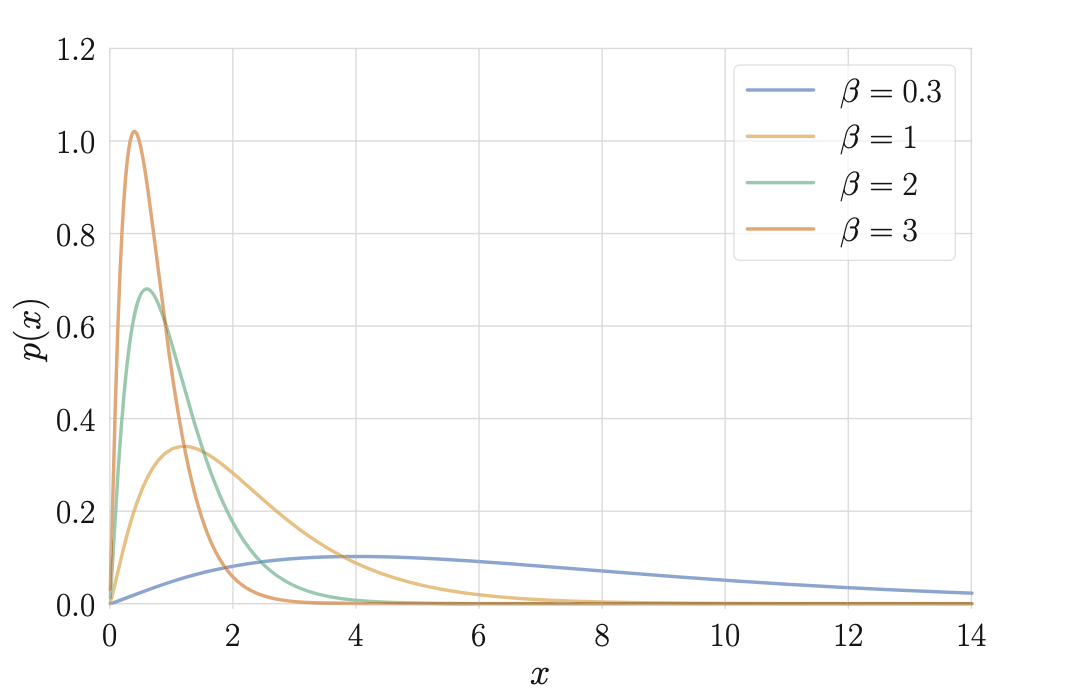
\includegraphics[width=\linewidth]{gamma_family}
		\caption*{\textbf{(a)}}
	\end{minipage}
	\begin{minipage}[b]{0.49\linewidth}
      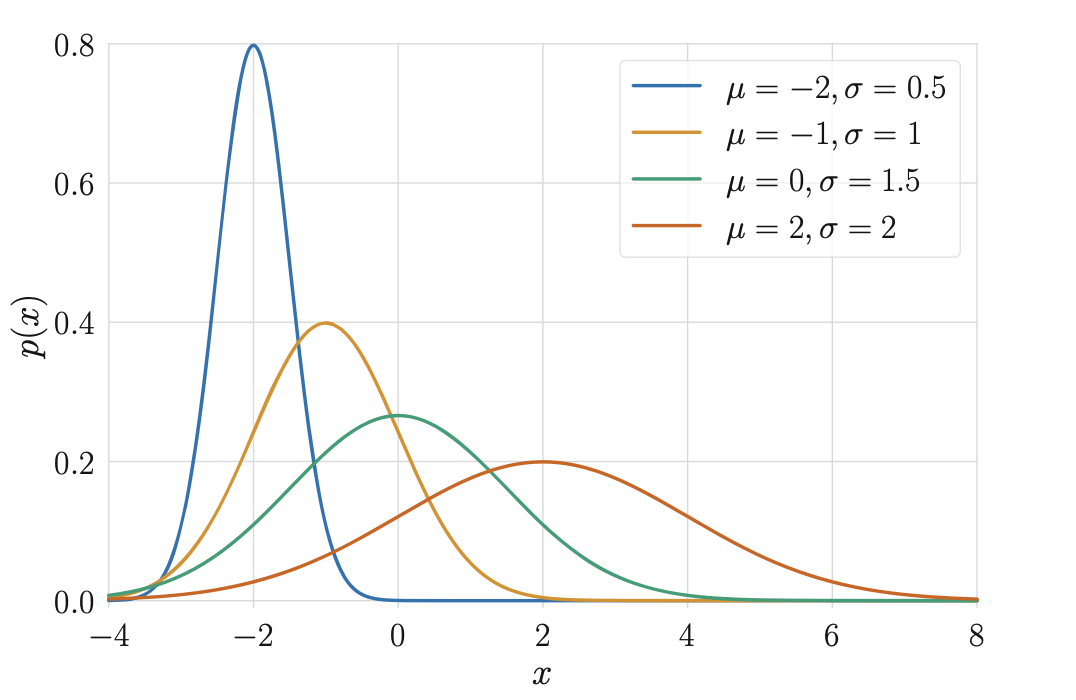
\includegraphics[width=\linewidth]{gaussian_family}
		\caption*{\textbf{(b)}}
	\end{minipage}
	\caption{Illustration of location-scale families for the Gamma distribution and the Gaussian distribution, respectively. In the parametrization of the the Gamma function with the rate parameter $\b$, the scale parameter as defined in Theorem \ref{theorem:pdf_gen} is actually $\s = 1/\b$. Note that as the scale $\s$ increases the distribution becomes less concentrated around the location parameter $\m$. In particular, $\lim_{\s\to\infty} p(x; \m,\s) = \d(x-\m)$. \textbf{(a)} Members of the same scale family of Gamma distributions with shape parameter $\a = 2.2$. \textbf{(b)} Members of the same location-scale family of Gaussian distributions.}\label{fig:pdf_gen}
\end{center}
\end{figure}

\chapter{Autoencoders}\label{chap:ae}

Having introduced the basics of neural networks in chapter \ref{preliminary} we can consider a specific architecture of a neural network, a so called autoencoding neural network, or short: autoencoder. The idea of autoencoders is to take a given input, compress the input to a smaller size (usually called encoding) and afterwards, expand it as accurately as possible to the original size again (usually called decoding). Such an architecture is widely used in different applications. For example on social media platforms, where users send images to one another. Instead of sending the original image, which size might very well be a couple of megabytes, the image is firstly being encoded and sent in the compressed representation. Afterwards, the recipient decodes the image to its original representation. This way one has only to transmit the encoded representation, which usually is smaller by magnitudes.
Another very important application of autoencoders is in the machine learning field. Most state of the art machine learning models are using autoencoding structures, since it is way more efficient to first encode the data and then run a model on the encoded data. This is quite straight-forward, considering the same argument as in the previous use case - the encoded data being smaller by magnitudes. This way processing the samples can happen much faster compared to the non-encoded data samples and secondly, it makes storing data (on the drive and in memory) much more efficient.\\
In this chapter we want to consider how to formulate autoencoding neural networks from a mathematical point of view, take a look at some important results and lastly, analyse the theory in multiple applications using Python.

\section{Conceptional ideas}

As already mentioned, an autoencoding neural network first compresses/encodes the input data to a smaller representation. The size of this smaller representation is usually referred to as bottleneck of the autoencoder.
Afterwards, the autoencoding neural network expands/decodes the data to its original size. Hence, we can divide these two steps into separate architectures - the encoding and the decoding part of the neural network, which we will formulate separately.\\
In figure \ref{autoencoder} we can take a look at a visual example of an autoencoding architecture.


\begin{figure}
\begin{center}
   \begin{minipage}[b]{0.9\linewidth}
      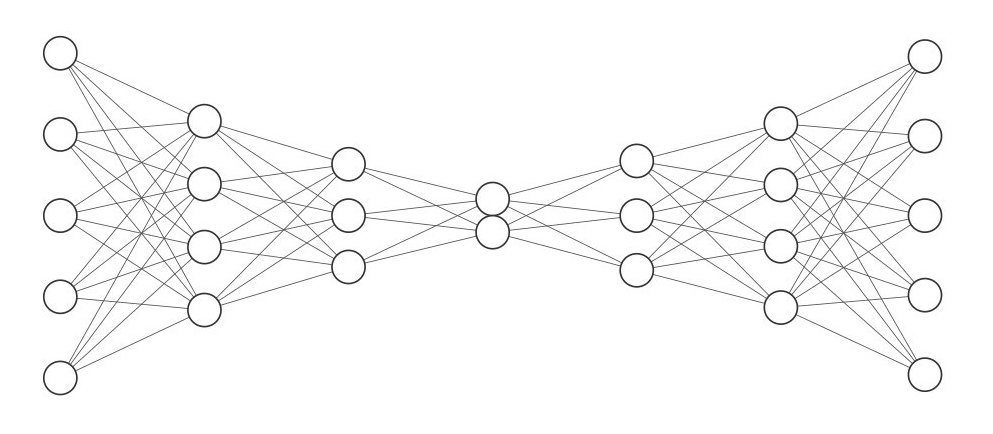
\includegraphics[width=\linewidth]{autoencoder}
      \caption{An autoencoding neural network with input and output $x, y\in \R^5$. The five hidden layers have dimensions $4$, $3$, $2$, $3$ and $4$ respectively. Hence, the bottleneck dimension is $2$ in this example. The graphic was generated with http://alexlenail.me/NN-SVG/index.html}\label{autoencoder}
	\end{minipage}
\end{center}
\end{figure}


If we divide the autoencoding structure as described above, we firstly obtain the encoder as we can see in figure \ref{img_encoder} or formally defined as follows.

\begin{definition}\label{def_encoder}
Let $\T$ be a parameter space and $\t \in \T$ a set of parameters, $L\in \N$ and $d_1,\ldots, d_L\in\N$. Let further $\f$ be an activation function and $f_{\f,L,\t}$ a neural network.\\
If the neural network $f_{\f,L,\t}$ fulfils the condition $n_i= d_1 \geq \ldots \geq d_L = n_o$ with $n_i, n_o \in \N$ being the input and output dimensions respectively, then we speak of an \textbf{encoding neural network} (or short: \textbf{encoder}) and denote it as $f_e$.
\end{definition}


\begin{figure}
\begin{center}
   \begin{minipage}[b]{0.9\linewidth}
      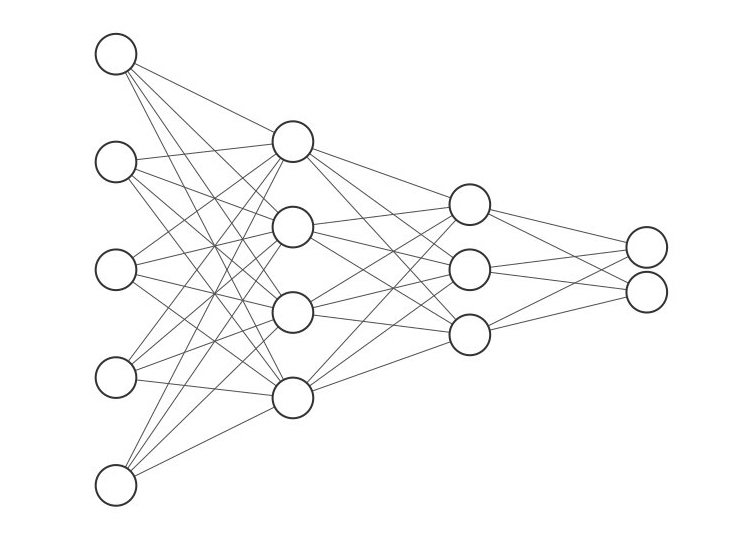
\includegraphics[width=\linewidth]{encoder}
      \caption{An encoding neural network with input $x\in \R^5$ and output $y \in \R^2$. The two hidden layers have dimensions $4$ and $3$. Hence, the encoder reduces the data dimensionality from $5$ to $2$ dimension. The graphic was generated with http://alexlenail.me/NN-SVG/index.html}\label{img_encoder}
	\end{minipage}
\end{center}
\end{figure}


For the second part of the divided autoencoding structure, we obtain the decoder as we can see in figure \ref{img_decoder}. We can define this architecture analogously to the encoder in definition \ref{def_encoder}.


\begin{definition}\label{def_decoder}
Let $\T$ be a parameter space and $\t \in \T$ a parameter, $L\in \N$ and $d_1,\ldots, d_L\in\N$. Let further $\f$ be an activation function and $f_{\f,L,\t}$ a neural network.\\
If the neural network $f_{\f,L,\t}$ fulfils the condition $n_i= d_1 \leq \ldots \leq d_L = n_o$ with $n_i, n_o \in \N$ being the input and output dimensions respectively, then we speak of an \textbf{decoding neural network} (or short: \textbf{decoder}).
\end{definition}


\begin{figure}
\begin{center}
   \begin{minipage}[b]{0.9\linewidth}
      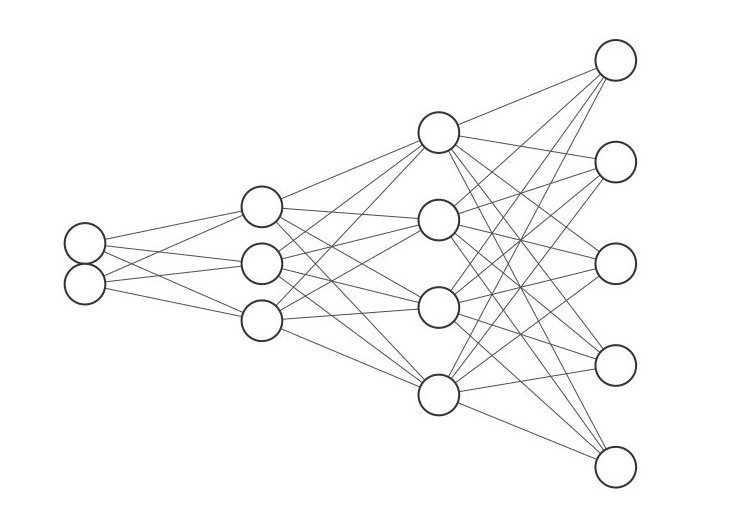
\includegraphics[width=\linewidth]{decoder}
      \caption{A decoding neural network with input $x\in \R^2$ and output $y \in \R^5$. The two hidden layers have dimensions $3$ and $4$. Hence, the decoder expands the data dimensionality from $2$ to $5$ dimensions. The graphic was generated with http://alexlenail.me/NN-SVG/index.html}\label{img_decoder}
	\end{minipage}
\end{center}
\end{figure}

Before combining the encoding and the decoding structure to obtain the autoencoding neural network, we need to consider the following technicality first.

\begin{lemma}\label{lemma:composition_of_nns}
Let $f_1, f_2$ be two neural networks of depths $L_1, L_2 \in \N$ with parameters $\t_1, \t_2 \in \T$, where $\T$ is an arbitrary parameter space. Furthermore, let the dimensions of each layer be $d_1, \ldots, d_{L_1} \in \N$ of $f_1$ and $\tilde{d}_1, \ldots, \tilde{d}_{L_2} \in \N$ of $f_2$. Additionally, let $d_{L_1} = \tilde{d}_1$.\\
Then their composition $f_2\circ f_1$ is a neural network of depth $L_1 + L_2$ with parameters $(\t_1, \t_2)$.
\end{lemma}

\begin{proof}
Since $f_1$ is a neural network of depth $L_1$ with parameters $\t_1$, its architecture looks like
\begin{align}\label{nn_1}
f_1 (x) = H_{L_1} \circ H_{L_1-1} \circ \ldots H_{2} \circ H_1 (x),\qquad x \in \R^{d_1}.
\end{align}
Analogously, we can write $f_2$ as
\begin{align}\label{nn_2}
f_2 (y) = \tilde{H}_{L_2} \circ \tilde{H}_{L_2-1} \circ \ldots \tilde{H}_{2} \circ \tilde{H}_1 (y), \qquad y \in \R^{\tilde{d}_1}.
\end{align}
Since we assumed that the output dimension $d_{L_1}$ of the neural network $f_1$ is equal to the input dimension $\tilde{d}_1$ of the neural network $f_2$, we can consider the result of \eqref{nn_1} as input for \eqref{nn_2}
\begin{align*}
y &\coloneqq H_{L_1} \circ H_{L_1-1} \circ \ldots H_{2} \circ H_1 (x), \qquad x \in \R^{d_1}.
\end{align*}
Hence, we obtain
\begin{align}\label{nn_comp}
f_2 (y) &= \tilde{H}_{L_2} \circ \tilde{H}_{L_2-1} \circ \ldots \tilde{H}_{2} \circ \tilde{H}_1 (y),\nonumber\\
f_2\left(f_1\left(x\right)\right)  &= \tilde{H}_{L_2} \circ \tilde{H}_{L_2-1} \circ \ldots \tilde{H}_{2} \circ \tilde{H}_1 \left( H_{L_1} \circ H_{L_1-1} \circ \ldots H_{2} \circ H_1 (x) \right),\nonumber\\
f_2\left(f_1\left(x\right)\right)  &= \tilde{H}_{L_2} \circ \tilde{H}_{L_2-1} \circ \ldots \tilde{H}_{2} \circ \tilde{H}_1 \circ H_{L_1} \circ H_{L_1-1} \circ \ldots H_{2} \circ H_1 (x), \qquad x \in \R^{d_1}.
\end{align}
Therefore, from \eqref{nn_comp} follows that the composition $f_2 \circ f_1$ is a neural network of depth $L_1 + L_2$.\\
Lastly, we consider the parameters $\t$ of the neural network $f_2 \circ f_1$. Since the parameters of a neural network were defined as $\t = (\t_1,\ldots, \t_L)$, where each entry is defined as $\t_i = (W_i, b_i)$ and denotes the weight and bias of each layer $H_i$ or $\tilde{H}_i$, respectively, we can write the parameters of both neural networks as
\begin{align*}
\t_1 &\coloneqq (\t_1, \ldots, \t_{L_1}) = \left((W_1, b_1),\ldots, (W_{L_1}, b_{L_1}) \right),\\
\t_2 &\coloneqq (\tilde{\t}_1, \ldots, \tilde{\t}_{L_2}) = \left((\tilde{W}_1, \tilde{b}_1),\ldots, (\tilde{W}_{L_2}, \tilde{b}_{L_2}) \right).
\end{align*}
Hence, the composition $f_2\circ f_1$ has the parameters
\begin{align*}
\t  &= \left((W_1, b_1),\ldots, (W_{L_1}, b_{L_1}), (\tilde{W}_1, \tilde{b}_1),\ldots, (\tilde{W}_{L_2}, \tilde{b}_{L_2})  \right)\\
&= \left(\t_1,\ldots \t_{L_1}, \tilde{\t}_1, \ldots, \tilde{\t}_{L_2} \right) \eqqcolon \left(\t_1,\t_2 \right).
\end{align*}
\end{proof}


Lemma \ref{lemma:composition_of_nns} allows us to consider a modern approach to neural networks, a so called modular approach. Essentially, we consider entire structures like the encoding and the decoding neural network as a self-contained module. These modules can now easily be put together by considering them in series. This is very useful in practice, since modern neural networks consist of thousands of layers and thus billions of parameters. Considering a modular approach one can therefore divide the whole neural network and tune each module separately.


\begin{theorem}
Let $\T$ be a parameter space, $N\in \N$ and $L_1,\ldots,L_N\in \N$. Furthermore, let $f_1,\ldots,f_N$ be neural networks with parameters $\t_1,\ldots,\t_N\in\T$ and depths $L_1,\ldots,L_N$, respectively. Lastly, let the output dimension of $f_i$ match the input dimension of $f_{i+1}$ for all $i\in\{1,\ldots,N-1\}$.\\
Then the composition
\begin{align*}
f \coloneqq f_{N} \circ f_{N-1} \circ \ldots \circ f_1,
\end{align*}
is a neural network with parameters $\t = (\t_1,\ldots\t_N)$ of depth $L = L_1 + \ldots + L_N$.
\end{theorem}


\begin{proof}
Applying lemma \ref{lemma:composition_of_nns} to $f_1$ and $f_2$ yields the composed neural network $f^{(1)} \coloneqq f_2 \circ f_1$ with parameters $\t^{(1)} \coloneqq (\t_1, \t_2)$ and depth $L^{(1)}\coloneqq L_1 + L_2$.\\
If we now apply lemma \ref{lemma:composition_of_nns} once again to $f^{(1)}$ and $f_3$, we receive $f^{(2)} \coloneqq f_3 \circ f^{(1)}$ with parameters $\t^{(2)} \coloneqq (\t^{(1)}, \t_3) = (\t_1, \t_2, \t_3)$ and depth $L^{(2)}\coloneqq L^{(1)} + L_3 = L_1 + L_2 + L_3$.\\
We realize, that iteratively applying lemma \ref{lemma:composition_of_nns} yields  after $N-1$ applications
\begin{align*}
f^{(N-1)} &= f_{N} \circ f_{N-1} \circ \ldots \circ f_1,\\
\t^{(N-1)}&= \left(\t_1, \ldots, \t_N \right),\\
L^{(N-1)} &= \sum_{i=1}^{N-1} L_i.
\end{align*}
Therefore the assertion is proven.
\end{proof}


\begin{definition}\label{def_autoencoder}
Let $f_e$ and $f_d$ be an encoding and a decoding neural network with input dimension $n_i$ in $\N$ and output of the encoding neural network $n_b$ in $\N$, that we will refer to as \textbf{bottleneck} of the autoencoding neural network.
Then we define an \textbf{autoencoding neural network} $f_a$ as the composition
\begin{align*}
f_a: \R^{n_i} &\to \R^{n_i},\\
x &\mapsto \left(f_d \circ f_e \right)(x).
\end{align*}
\end{definition}

\begin{remark}
Let $f_e$ and $f_d$ be an encoding and a decoding neural network as in definition \ref{def_autoencoder}. Then the composition $f_d \circ f_e$ is indeed a neural network, following from lemma \ref{lemma:composition_of_nns}.
\end{remark}


\section{Training of autoencoders}

When tackling the question of how to train an autoencoding neural network, we realize that in contrast to regular neural networks, where we compare the output of the neural network to a label, in the current setting we can compare the input data to the computed output, since the goal of an autoencoding neural network ultimately is to alter and reconstruct images. In other words, we approach this optimization problem in an unsupervised learning setting. This forces us to consider slightly different loss functions than in the supervised learning setting.


\begin{definition}
Let $X, Y$ be Banach spaces representing the input and output space, respectively.\\
Then a continuous function defined as
\begin{align*}
L:X\times Y &\to \R,\\
\left(x, p(x)\right) &\mapsto L\left(x, p(x)\right),
\end{align*}
is called \textbf{unsupervised loss function}.
\end{definition}


There are multiple important loss functions in computer vision. We will consider a couple of those in the following example. For further reading please take a look at \cite{foster2022generative}


\begin{example}
Let $\O$ be a pixel domain with resolution $(M,N)$ and $d$ the number of channels. Furthermore, let $f$ be a neural network with arbitrary but fixed architecture.\\
Then the following functions are loss functions operating on images.
\begin{mydescription}{\widthof{\textbf{Binary Cross-Entropy (BCE)}}}
\item[\textbf{Mean Squared Error (MSE)}] \begin{align*}
\MSE(\p, f(\p)) = \sum_{i=1}^{M}\sum_{j=1}^{N}\left\|\p_{ij} - f(\p)_{ij}\right\|^2,
\end{align*}
\item[\textbf{Binary Cross-Entropy (BCE)}]
\begin{align*}
\BCE(\p, f(\p)) = - \frac{1}{MN}\sum_{i=1}^{M}\sum_{j=1}^{N} \biggl(&\p_{ij} \log\left(f\left(\p\right)_{ij}\right)\\ + \bigl(1-&\p_{ij}\bigr)\log\left(1 - f\left(\p\right)_{ij}\right)\biggr),
\end{align*}
\end{mydescription}
where $\p$ denotes an image defined on $\P_{\O}$.
\end{example}


\begin{remark}
The Binary Cross-Entropy loss function is usually used for binary classification problems. However, it still works in computer vision.
\end{remark}


\section{Applications}

In this section we want to train a couple of own autoencoding neural networks on the MNIST dataset - a dataset consisting of handwritten digits. Lastly, we will consider a composition of MNIST images in order to simulate a scenario that will allow the Duckeneers GmbH to generate new data. We will consider some various architectures of neural networks and visualise the results in a comprehensible manner.\\
First, we want to consider the most simple architecture, a fully connected linear neural network.

\begin{definition}\label{def_linear_encoder}
Let $\T$ be an arbitrary parameter space, $L\in \N$ and $d_1,\ldots,d_L \in \N$. Furthermore, let $\f$ be an arbitrary activation function.\\
Then an encoding neural network, where each layer $H_1,\ldots, H_L$ is defined as
\begin{align*}
H_i(x) = \hat{\f}(W_ix + b_i), \qquad x \in \R^{d_i}, i \in \{1,\ldots, L\},
\end{align*}
where $\t_i = (W_i, b_i)\in\T$ are the parameters of the $i$-th layer, see \eqref{eq_linear_layer}. Such an encoding neural network is called a \textbf{linear encoder}.
\end{definition}

Analogously, we define a linear decoding neural network.

\begin{definition}\label{def_linear_decoder}
Let $\T$ be an arbitrary parameter space, $L\in \N$ and $d_1,\ldots,d_L \in \N$. Furthermore, let $\f$ be an arbitrary activation function.\\
Then a decoding neural network, where each layer $H_1,\ldots, H_L$ is defined as
\begin{align*}
H_i(x) = \hat{\f}(W_ix + b_i), \qquad x \in \R^{d_i}, i \in \{1,\ldots, L\},
\end{align*}
where $\t_i=(W_i, b_i)\in\T$ are the parameters of the $i$-th layer $H_i$, see \eqref{eq_linear_layer}. Such a decoding neural network is called a \textbf{linear decoder}.
\end{definition}


With the definitions of the linear encoder and linear decoder, we now can define a linear autoencoder.


\begin{definition}
Let $f_e$ and $f_d$ be a linear encoder and a linear decoder. Then a \textbf{linear autoencoder} $f_{\text{lin}}$ is defined as the composition
\begin{align*}
f_{\text{lin}} \coloneqq f_d \circ f_e.
\end{align*}
\end{definition}

Before considering specific examples on the MNIST dataset, we need to consider some properties of the said dataset first.

\begin{remark}\label{def:mnist}
The MNIST dataset $\D$ consists of greyscale images with a resolution of $(28,28)$. Hence, the images are defined on the pixel domain $\O$ of $\D$ with $\O=\{1,\ldots,28\}\times\{1,\ldots,28\}$ with only one channel.
\end{remark}

Now, let us take a look at a specific example of a linear autoencoder defined on the MNIST dataset.

\begin{algorithm}
Let the input and output dimensions be $n_i, n_o \in\N$. Furthermore, let the linear encoder and the linear decoder have $k$ hidden linear layers with dimensions $n_1, n_2,\ldots, n_k\in\N$ with bottleneck $n_b\in\N$.\\
Let the chosen optimizer be ADAM first and afterwards be AMSGrad with a learning rate $\g=\num{3e-4}$ and the MSE loss function. We will perform the training on $10.000$ epochs with a batch size of $512$.
\caption{Linear Autoencoder}\label{alg:linear_AE}
\begin{algorithmic}[1]
\Require $\g \gets \num{3e-4}$
\For{epoch in $\{1,\ldots, 10.000\}$}
	\For{image in batch}
		\State image = image.reshape(784) \Comment{Convert the image from matrix to array.}
	    \State encoded = encoder(image) \Comment{Encode the image onto latent space.}
		\State reconstructed = decoder(encoded) \Comment{Decode the encoded image.}
    	\State loss = MSE(reconstructed, image) \Comment{Compare the output to the input.}
	    \State optimization(loss, $\g$) \Comment{Perform an optimization step.}
    \EndFor
\EndFor
\end{algorithmic}
\end{algorithm}


Let's take a look at the trained autoencoders using the ADAM and the AMSGrad optimizer. In figure \ref{fig:linear_AE_2d_latent} we can see the latent space of the models. Furthermore, in figure \ref{fig:linear_AE_2d_inference} we can see ten reconstructions for each of the ten digits. The training progresses are illustrated in figure \ref{fig:linear_AE_2d_adam_training_progress} with the ADAM optimizer and in figure \ref{fig:linear_AE_2d_amsgrad_training_progress} with an AMSGrad optimizer, respectively.


\begin{figure}
\begin{center}
   \begin{minipage}[b]{0.49\linewidth}
      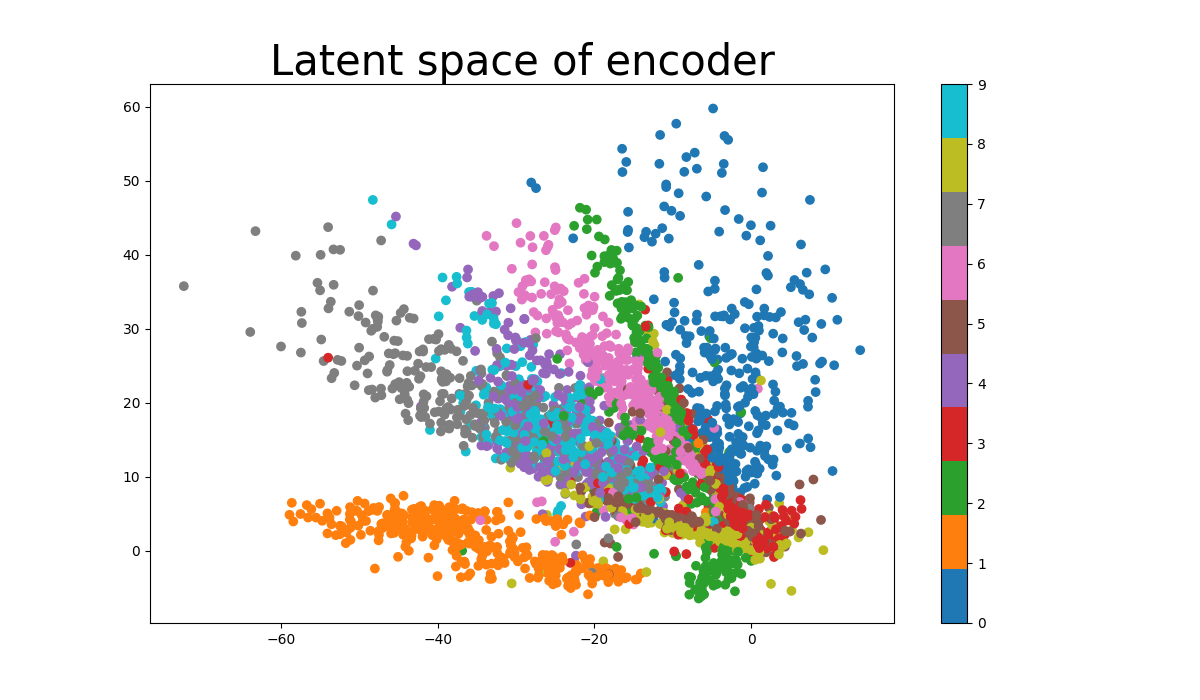
\includegraphics[width=\linewidth]{linear_AE_2d_adam_latent}
	\end{minipage}
	\begin{minipage}[b]{0.49\linewidth}
      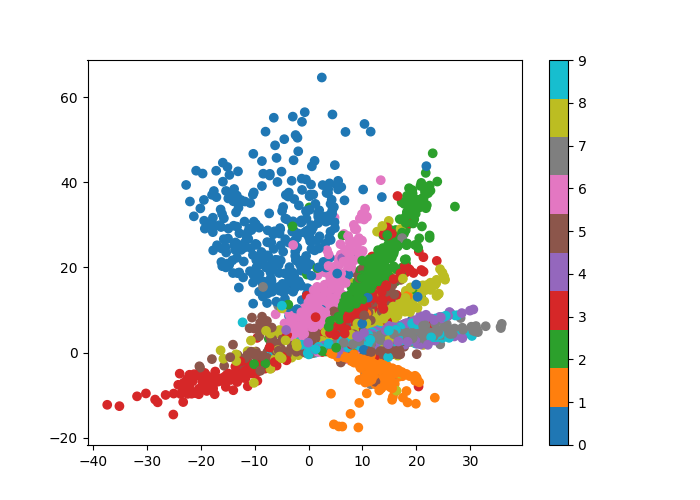
\includegraphics[width=\linewidth]{linear_AE_2d_amsgrad_latent}
	\end{minipage}
\end{center}
\caption{The figure illustrates the latent space of the linear autoencoder with bottleneck $n_b=2$ optimized with an ADAM optimizer (left) and an AMSGrad optimizer (right). Each dot is one encoded image of a digit. The color and the corresponding color map represent the digit that was encoded.}\label{fig:linear_AE_2d_latent}
\end{figure}


\begin{figure}
\begin{center}
   \begin{minipage}[b]{0.49\linewidth}
      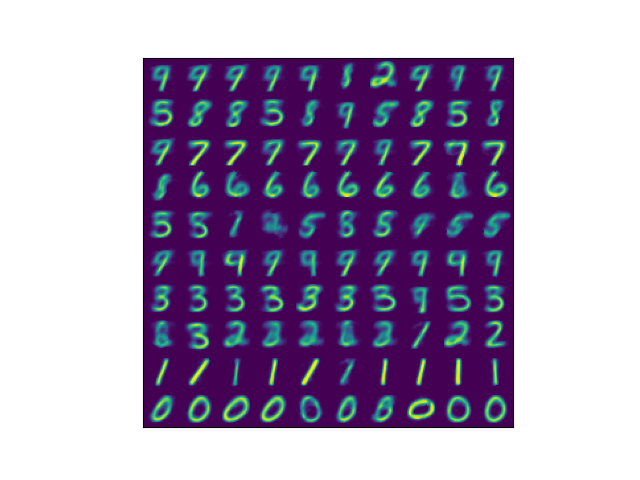
\includegraphics[width=\linewidth]{linear_AE_2d_adam_inference}
	\end{minipage}
   \begin{minipage}[b]{0.49\linewidth}
      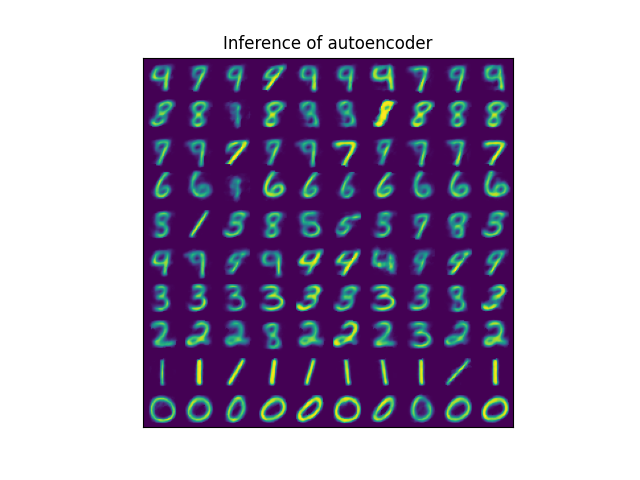
\includegraphics[width=\linewidth]{linear_AE_2d_amsgrad_inference}
	\end{minipage}
\end{center}
\caption{The figure illustrates the inference of the linear autoencoder with bottleneck $n_b=2$ optimized with an ADAM optimizer (left) and an AMSGrad optimizer (right). The inference are ten reconstructed images for each of the ten digits.}\label{fig:linear_AE_2d_inference}
\end{figure}


\begin{figure}
\begin{center}
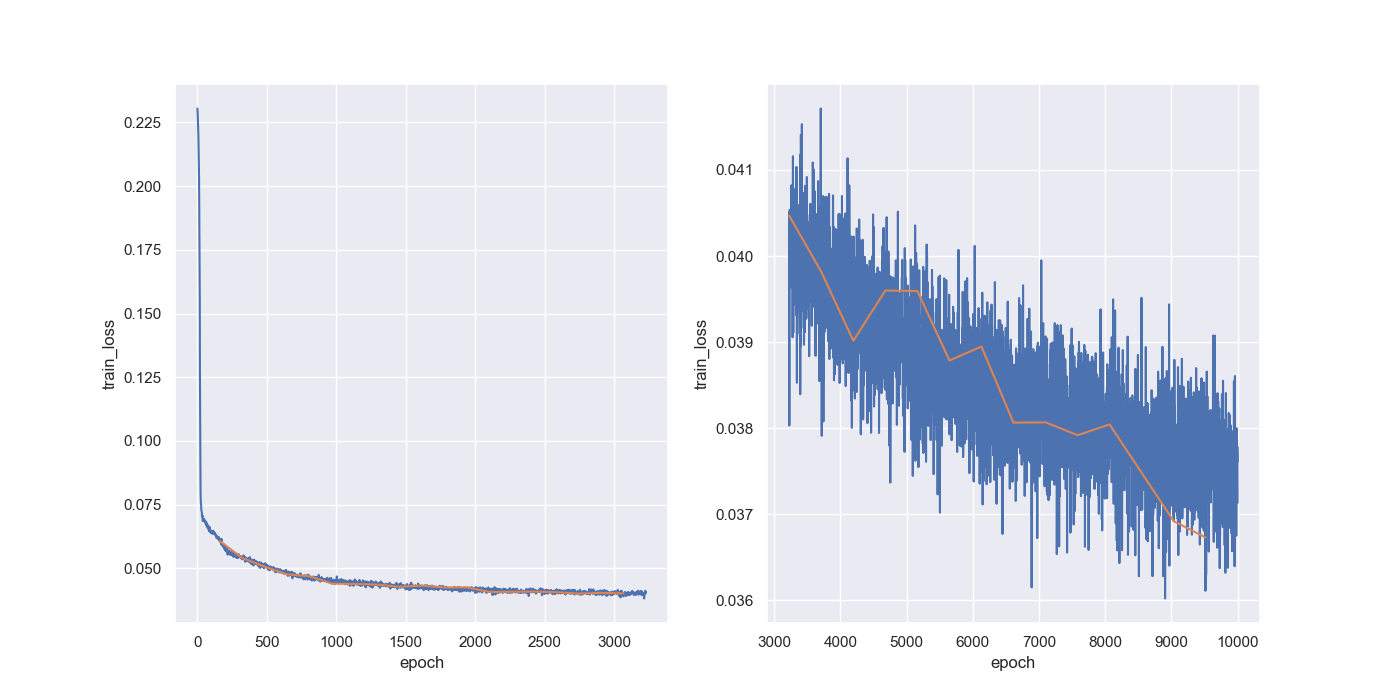
\includegraphics[width=\linewidth]{linear_AE_2d_adam_training_progress}
\end{center}
\caption{The figure illustrates the training progresses of the linear autoencoder with bottleneck $n_b=2$ optimized with an ADAM optimizer with epochs on one axis and corresponding training loss on the other axis.On the left side we see the first $3.500$ epochs and on the right side the following epochs until $10.000$. The blue line represents the loss in each epoch and the orange line represents the moving average over $100$ epochs to point out the trend of the training progress.}\label{fig:linear_AE_2d_adam_training_progress}
\end{figure}


\begin{figure}
\begin{center}
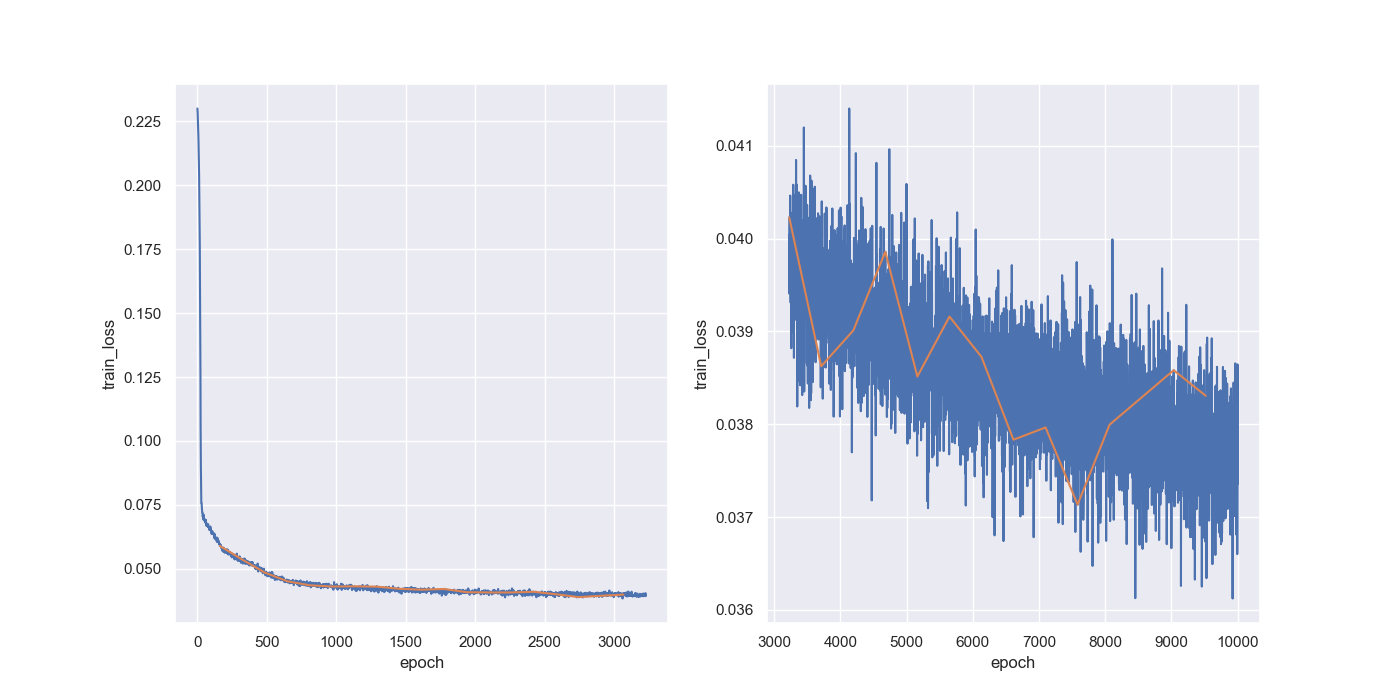
\includegraphics[width=\linewidth]{linear_AE_2d_amsgrad_training_progress}
\end{center}
\caption{The figure illustrates the training progresses of the linear autoencoder with bottleneck $n_b=2$ optimized with an AMSGrad optimizer with epochs on one axis and corresponding training loss on the other axis.On the left side we see the first $3.500$ epochs and on the right side the following epochs until $10.000$. The blue line represents the loss in each epoch and the orange line represents the moving average over $100$ epochs to point out the trend of the training progress.}\label{fig:linear_AE_2d_amsgrad_training_progress}
\end{figure}


Now, let's consider another latent dimension, resulting in $3$ dimensions. This allows the neural network to save more information upon encoding the data and hence, it should be able to perform better reconstructions. However, it makes visualising the latent space a bit more difficult. In figure \ref{fig:linear_AE_3d_adam_latent} we can see the latent space of the autoencoder from two different perspectives trained with the ADAM optimizer and in figure \ref{fig:linear_AE_3d_amsgrad_latent} with the AMSGrad optimizer. Furthermore, in figure \ref{fig:linear_AE_3d_inference} we can see ten reconstructions for each of the ten digits. The training progress for the ADAM optimizer is illustrated in figure \ref{fig:linear_AE_3d_adam_training_progress} and for the AMSGrad optimizer in figure \ref{fig:linear_AE_3d_amsgrad_training_progress}, respectively.


\begin{figure}
\begin{center}
   \begin{minipage}[b]{0.49\linewidth}
      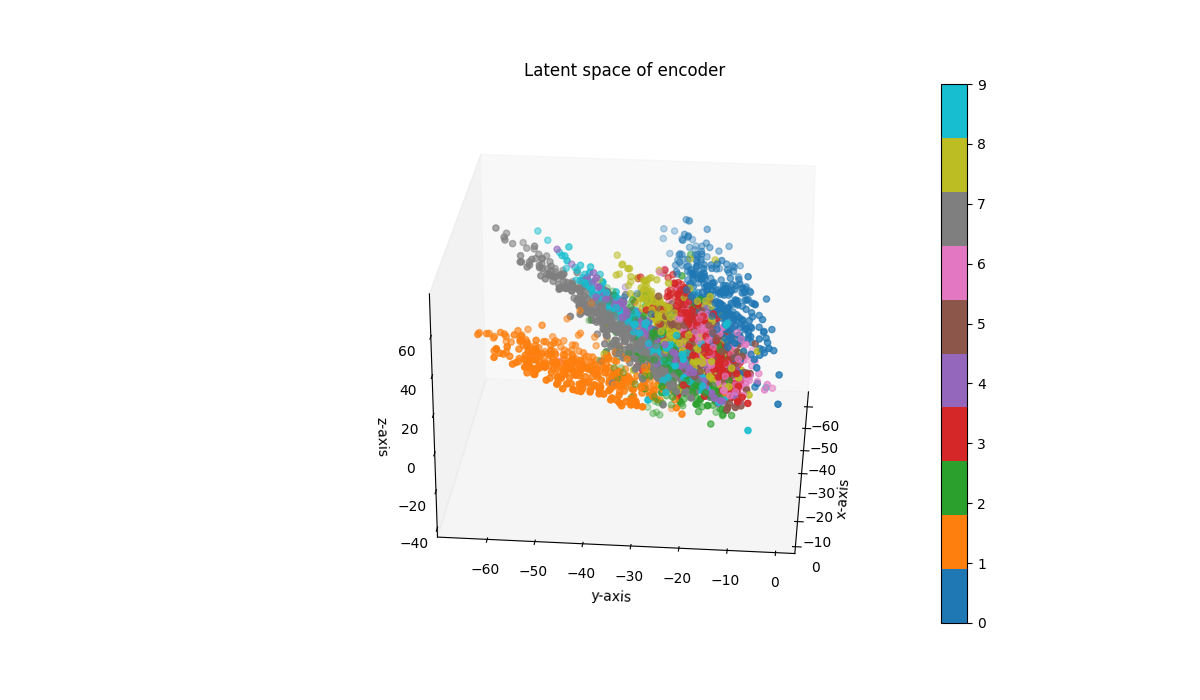
\includegraphics[width=\linewidth]{linear_AE_3d_adam_latent_1}
	\end{minipage}
	\begin{minipage}[b]{0.49\linewidth}
      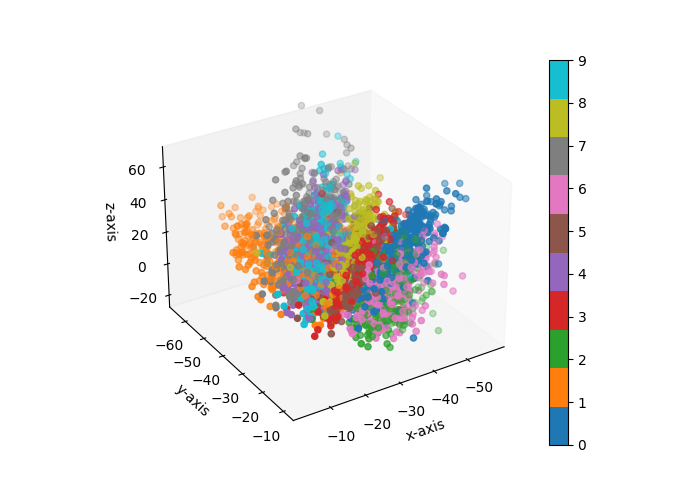
\includegraphics[width=\linewidth]{linear_AE_3d_adam_latent_2}
	\end{minipage}
\end{center}
\caption{The figure illustrates the latent space of the linear autoencoder with bottleneck $n_b=3$ optimized with an ADAM optimizer from two different perspectives. Each dot is one encoded image of a digit. The color and the corresponding color map represent the digit that was encoded.}\label{fig:linear_AE_3d_adam_latent}
\end{figure}

\begin{figure}
\begin{center}
   \begin{minipage}[b]{0.49\linewidth}
      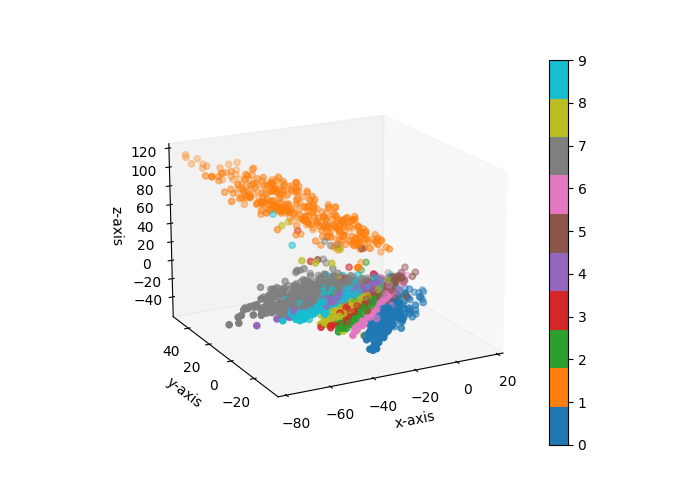
\includegraphics[width=\linewidth]{linear_AE_3d_amsgrad_latent_1}
	\end{minipage}
   \begin{minipage}[b]{0.49\linewidth}
      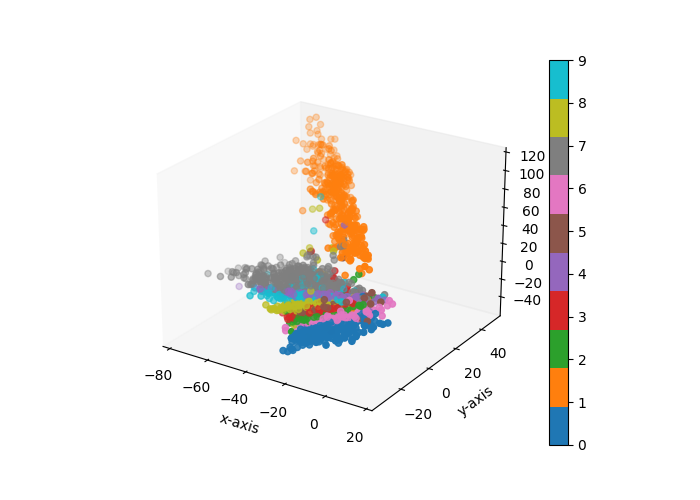
\includegraphics[width=\linewidth]{linear_AE_3d_amsgrad_latent_2}
	\end{minipage}
\end{center}
\caption{The figure illustrates the latent space of the linear autoencoder with bottleneck $n_b=3$ optimized with an AMSGrad optimizer from two different perspectives. Each dot is one encoded image of a digit. The color and the corresponding color map represent the digit that was encoded.}\label{fig:linear_AE_3d_amsgrad_latent}
\end{figure}


\begin{figure}
\begin{center}
   \begin{minipage}[b]{0.49\linewidth}
      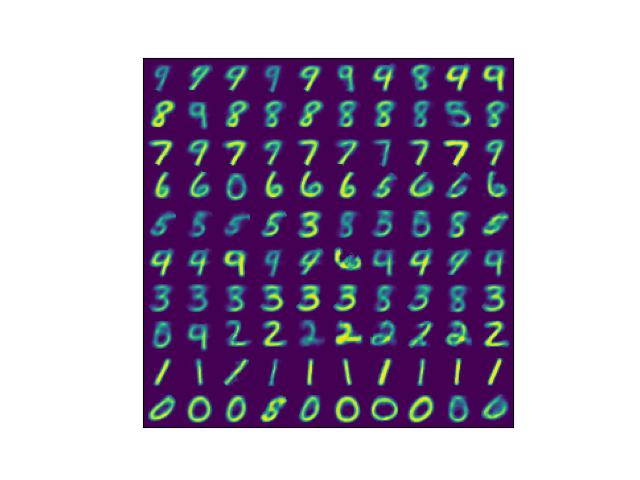
\includegraphics[width=\linewidth]{linear_AE_3d_adam_inference}
	\end{minipage}
   \begin{minipage}[b]{0.49\linewidth}
      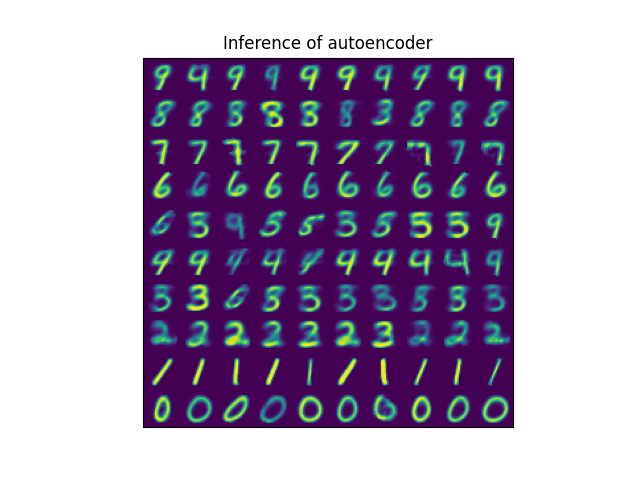
\includegraphics[width=\linewidth]{linear_AE_3d_amsgrad_inference}
	\end{minipage}
\end{center}
\caption{The figure illustrates the inference of the linear autoencoder with bottleneck $n_b=3$ optimized with an ADAM optimizer (left) and an AMSGrad optimizer (right). The inference are ten reconstructed images for each of the ten digits}.\label{fig:linear_AE_3d_inference}
\end{figure}


\begin{figure}
\begin{center}
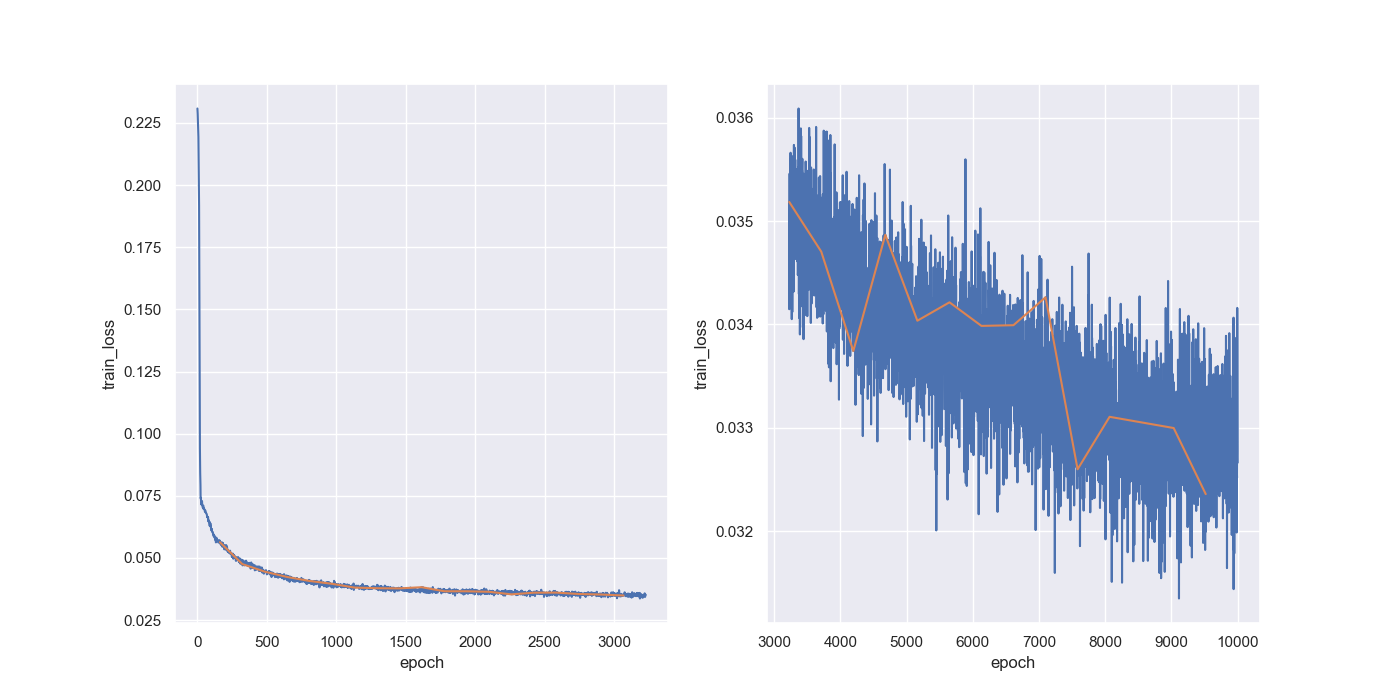
\includegraphics[width=\linewidth]{linear_AE_3d_adam_training_progress}
\end{center}
\caption{The figure illustrates the training progresses of the linear autoencoder with bottleneck $n_b=3$ optimized with an ADAM optimizer with epochs on one axis and corresponding training loss on the other axis.On the left side we see the first $3.500$ epochs and on the right side the following epochs until $10.000$. The blue line represents the loss in each epoch and the orange line represents the moving average over $100$ epochs to point out the trend of the training progress.}\label{fig:linear_AE_3d_adam_training_progress}
\end{figure}


\begin{figure}
\begin{center}
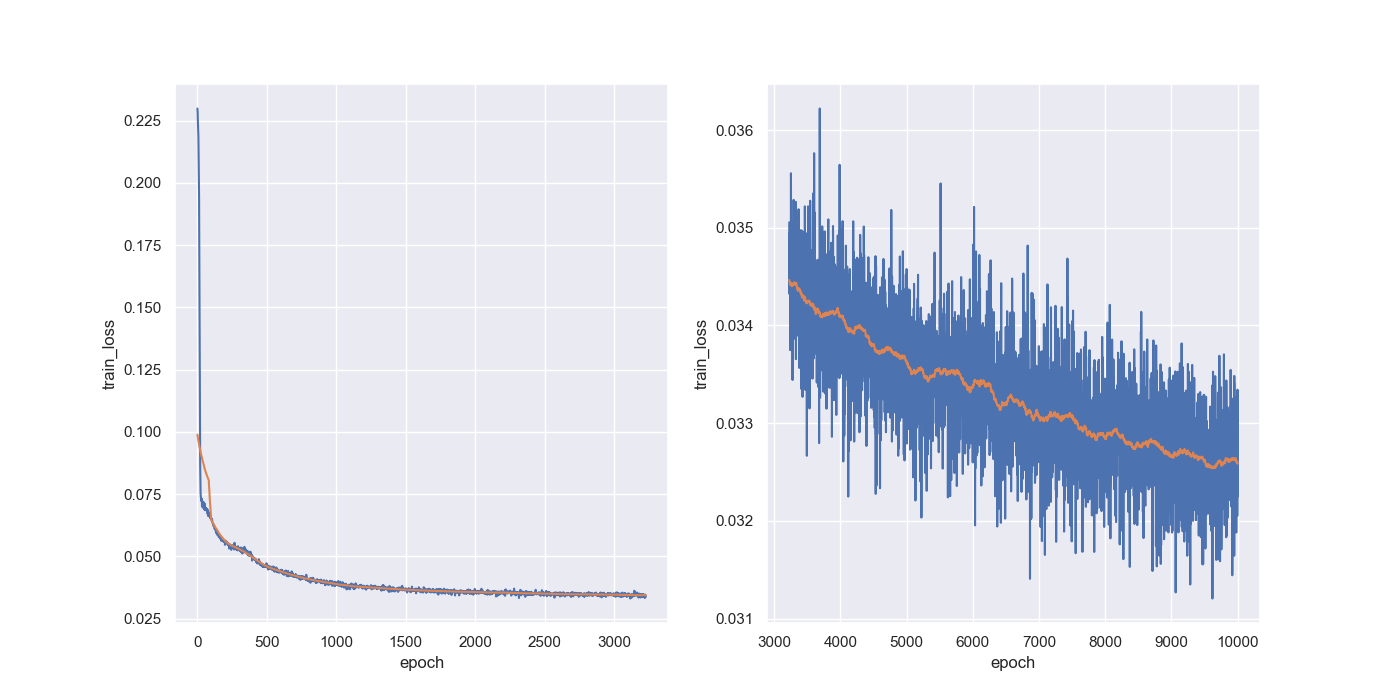
\includegraphics[width=\linewidth]{linear_AE_3d_amsgrad_training_progress}
\end{center}
\caption{The figure illustrates the training progresses of the linear autoencoder with bottleneck $n_b=3$ optimized with an AMSGrad optimizer with epochs on one axis and corresponding training loss on the other axis.On the left side we see the first $3.500$ epochs and on the right side the following epochs until $10.000$. The blue line represents the loss in each epoch and the orange line represents the moving average over $100$ epochs to point out the trend of the training progress.}\label{fig:linear_AE_3d_amsgrad_training_progress}
\end{figure}


As we saw in figure \ref{fig:linear_AE_3d_inference}, the linear autoencoder does produce recognisable digits in its reconstructions, but it still performs quite poorly. To address this issue, we propose another architecture of an autoencoding neural network. In this setting, we now consider convolutional layers instead of linear layers, this means that the connections between each layer are no longer matrix multiplications, but much more convolutions. Hence, we introduce the convolutional encoder and the convolutional decoder.


\begin{definition}\label{def_convolutional_encoder}
Let $\T$ be an arbitrary parameter space, $L\in \N$ and $d_1,\ldots,d_L \in \N$. Furthermore, let $\f$ be an arbitrary activation function.\\
Then an encoding neural network, where each layer $H_1,\ldots, H_L$ is defined as
\begin{align*}
H_i(x) = \hat{\f}(T_{\text{conv}, i}x + b_i), \qquad x \in \R^{d_i}, i \in \{1,\ldots, L\},
\end{align*}
where $\t_i = (T_{\text{conv}, i}, b_i)\in\T$ are the parameters of the $i$-th layer, see proposition \ref{prop:convolutional_layer}. Such an encoding neural network is called a \textbf{convolutional encoder}.
\end{definition}

Analogously, we define a convolutional decoding neural network.

\begin{definition}\label{def_convolutional_decoder}
Let $\T$ be an arbitrary parameter space, $L\in \N$ and $d_1,\ldots,d_L \in \N$. Furthermore, let $\f$ be an arbitrary activation function.\\
Then a decoding neural network, where each layer $H_1,\ldots, H_L$ is defined as
\begin{align*}
H_i(x) = \hat{\f}(T_{\text{conv}, i}x + b_i), \qquad x \in \R^{d_i}, i \in \{1,\ldots, L\},
\end{align*}
where $\t_i = (T_{\text{conv}, i}, b_i)\in\T$ are the parameters of the $i$-th layer, see proposition \ref{prop:convolutional_layer} Such a decoding neural network is called a \textbf{convolutional decoder}.
\end{definition}


Analogously to the linear autoencoder, we can define the convolutional autoencoder with the convolutional encoder and decoder architecture.

\begin{definition}
Let $f_e$ and $f_d$ be a convolutional encoder and a convolutional decoder. Then a \textbf{convolutional autoencoder} $f_{\text{conv}}$ is defined as the composition
\begin{align*}
f_{\text{conv}} \coloneqq f_d \circ f_e.
\end{align*}
\end{definition}

Now, lets define a specific example of a convolutional autoencoder and see how it performs.

\begin{algorithm}
Let the input and output dimensions be $n_i, n_o \in \N^{2\times 1}$. Furthermore, let the convolutional encoder and the convolutional decoder have $k$ hidden linear layers with dimensions $n_1, n_2,\ldots, n_k\in \N^{2\times 1}$ with bottleneck $n_b\in\N^{2\times 1}$. Here, $n_{b;1,2}\in\N^{2}$ represents the resolution and $n_{b,3}\in\N$ represents the number of channels in the corresponding layer, respectively.\\
Let the chosen optimizer be AMSGrad with a learning rate $\g=\num{3e-4}$ and the MSE loss function. We will perform the training on $10.000$ epochs.
\caption{Convolutional Autoencoder}\label{alg:convolutional_AE}
\begin{algorithmic}[1]
\Require $\g \gets \num{3e-4}$
\For{epoch in $\{1,\ldots, 10.000\}$}
	\For{image in batch}
	    \State encoded = encoder(image) \Comment{Encode the image onto latent space.}
		\State reconstructed = decoder(encoded) \Comment{Decode the encoded image.}
    	\State loss = MSE(reconstructed, image) \Comment{Compare the output to the input.}
	    \State optimization(loss, $\g$) \Comment{Perform an optimization step.}
    \EndFor
\EndFor
\end{algorithmic}
\end{algorithm}

However, in contrast to the linear autoencoder, the convolutional autoencoder architecture does not allow us to visualise the latent space as easily. The reason is that we designed our two linear autoencoders, each with distinct bottleneck dimensions of 2 and 3, respectively. This choice allowed us straightforward visualization of the latent space, given the single channel nature of our data, which was not altered in the course of computation. Unfortunately, the convolutional neural network does alter the amount of channels in the course of computation, such that we encode the data onto a resolution of one single pixel that comprises of $64$ channels and therefore, we would have to visualise $64$ channels.\\
We still came up with an idea of how to visualise the encoded representation, where we plot each channel in a separate bar in a bar plot, see figure \ref{fig:convolutional_AE_latent}. It is to be read in the following way: each digit receives an own representation in the latent space, that can be uniquely described by the composition of activations in each channel. Here, by activation we mean the value that each channel has. We see that most of the channels have quite different average values and so can be distinguished in that way.\\
However, what is highly interesting to highlight here is that although the magnitude of the values might differ quite significantly, their signs match most of the time.



\begin{figure}
\begin{center}
   \begin{minipage}[b]{\linewidth}
      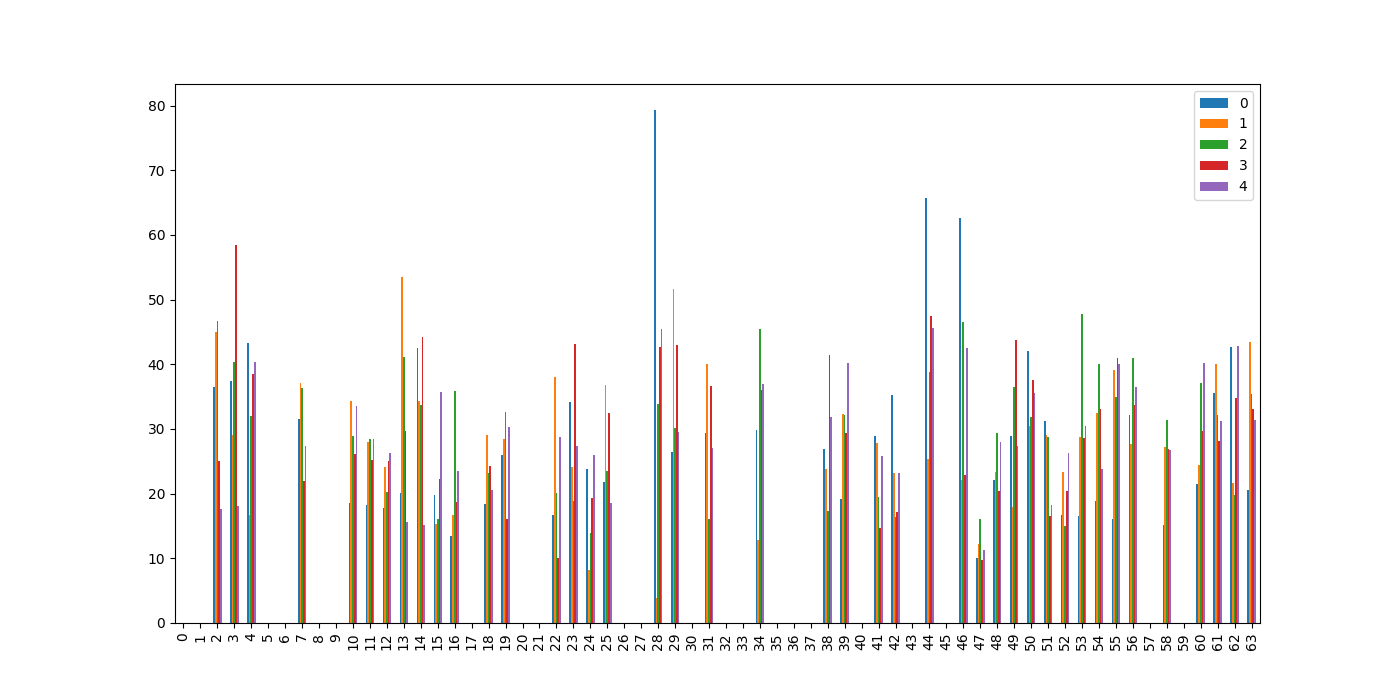
\includegraphics[width=\linewidth]{convolutional_AE_latent_0}
      This figure illustrates the average activations of each of the $64$ channels in the latent space of the convolutional autoencoder for the digits $0, 1, 2, 3$ and  $4$. The average has been taken over $5.000$ different images of the same digit.
	\end{minipage}
   \begin{minipage}[b]{\linewidth}
      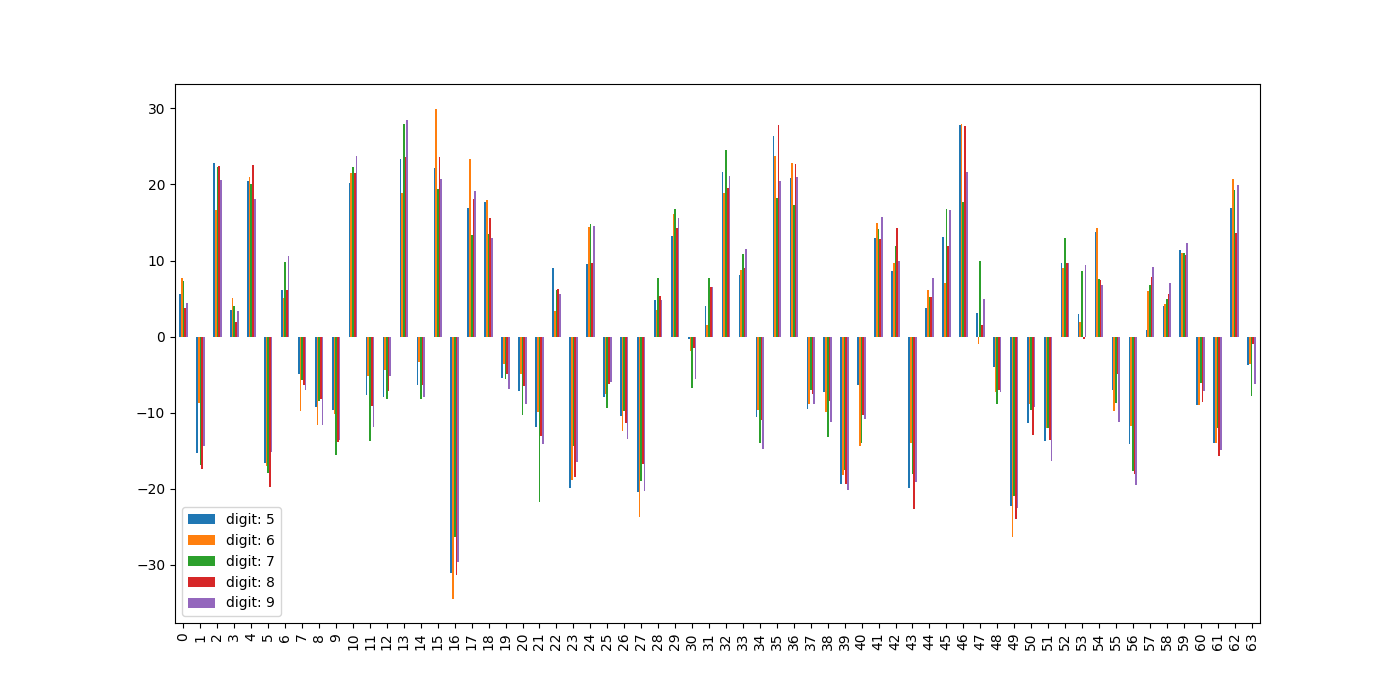
\includegraphics[width=\linewidth]{convolutional_AE_latent_1}
      This figure illustrates the average activations of each of the $64$ channels in the latent space of the convolutional autoencoder for the digits $5, 6, 7, 8$ and $9$. The average has been taken over $5.000$ different images of the same digit.
	\end{minipage}
\end{center}
\caption{The figure illustrates the activations of all $64$ channels in the latent space of our trained convolutional autoencoder, which was optimized with an AMSGrad optimizer, see algorithm \ref{alg:convolutional_AE}.}\label{fig:convolutional_AE_latent}
\end{figure}

Another interesting result that we want to highlight here is the inference of the convolutional autoencoder, which is displayed in figure \ref{fig:convolutional_AE_inference}. All reconstructions are sharp enough to be recognised as their original digit, which is a huge improvement compared to the inference of the linear autoencoder, see e.g. figure \ref{fig:linear_AE_3d_inference}.


\begin{figure}
\begin{center}
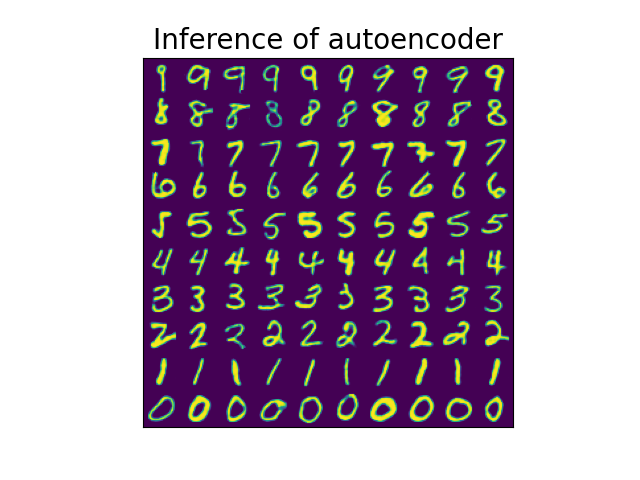
\includegraphics[width=0.7\linewidth]{convolutional_AE_inference}
\end{center}
\caption{The figure illustrates the inference of the convolutional autoencoder, optimized with the AMSGrad optimizer. The inference consists of the reconstructed images for each of the ten digits.}\label{fig:convolutional_AE_inference}
\end{figure}


Lastly, we want to take a quick look at the training progress of the convolutional autoencoder, see figure \ref{fig:convolutional_AE_training_progress}.

\begin{figure}
\begin{center}
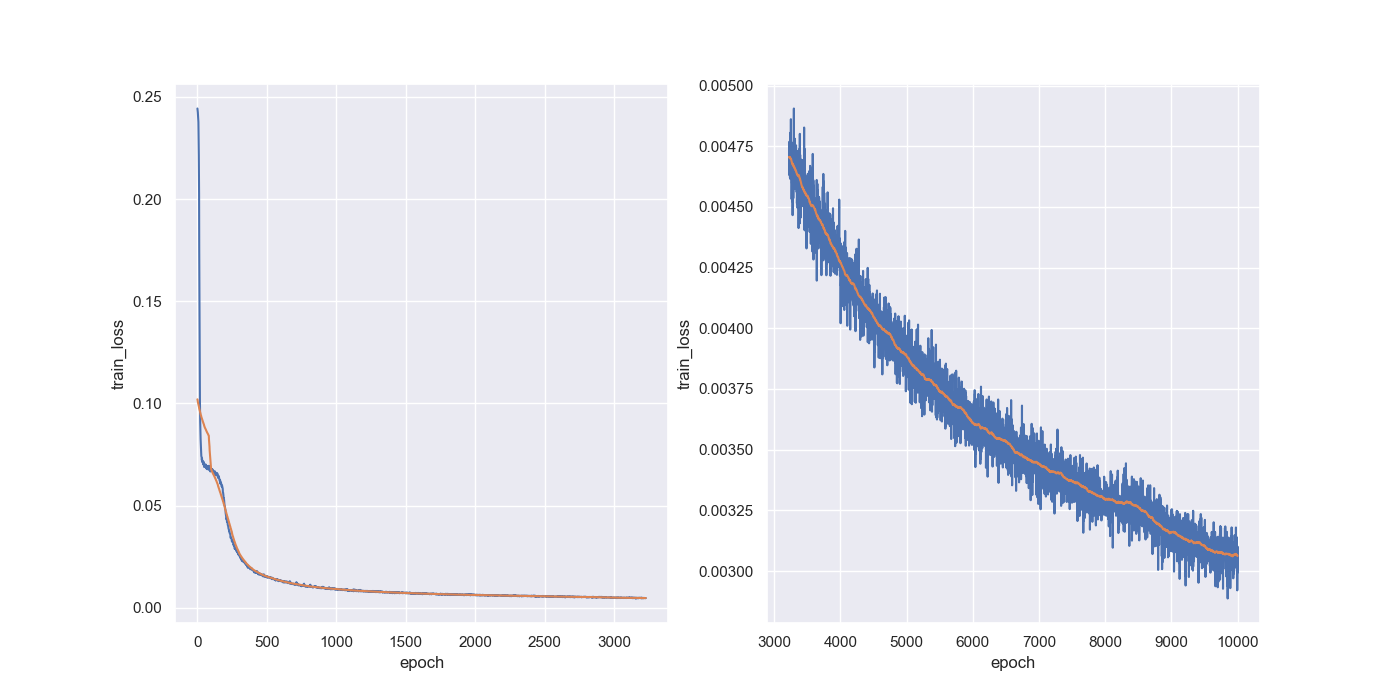
\includegraphics[width=\linewidth]{convolutional_AE_training_progress}
\end{center}
\caption{The figure illustrates the training progresses of the convolutional autoencoder optimized with an AMSGrad optimizer  with epochs on one axis and corresponding training loss on the other axis. On the left side we see the first $3.500$ epochs and on the right side the following epochs until $10.000$. The blue line represents the loss in each epoch and the orange line every $300$ epochs to point out the trend of the training progress.}\label{fig:convolutional_AE_training_progress}
\end{figure}

\iffalse
\include{convergence_rates}
\chapter{Implementation}

In this final chapter we want to consider a possible way to implement the theory. We postulate an algorithm how to apply the theory and afterwards, we construct a specific example of how to implement and visualize the theory.

\section{Algorithm}

In order to implement the theory, we have to consider the Tikhonov regularization method

\begin{align*}
\T_{\a;y_\d} = \min_{x \in D} \left( \D(\F(x), y_\d) + \a \reg(x) \right).
\end{align*}

Hence, we have to choose a certain similarity measure $\D: Y \times Y \to \R$, e.g.: $\D(y_1,y_2) = \frac{1}{2}\|y_1-y_2\|^2$ the mean squared error. Additionally, we have to define the regularizer. This we do by proposing for $q\geq 1$

\begin{align*}
\reg(\V,\wc) = \sum_{\l\in\L} \left\|\Phi_{\l}(\V,x) \right\|_{q}^q,
\end{align*}

with a neural network $\Phi(\V,\wc) = (\Phi(\V_\l,\wc))_{\l\in\L}$ as in equation \eqref{Def_Phi}. This ultimately resembles a non-linear $\ell^q$-regularizer. Combining the above two definitions, this leads to the optimization problem

\begin{align}\label{optim}
\T_{\a;y}(x) = \min_{x \in D} \left\{\frac{1}{2}\left\|\F(x) - y_\d\right\|^2 + \a \sum_{\l\in\L_l} \left\|\Phi_{\l}(\V,x) \right\|_{q}^q \right\}.
\end{align}

At this point, we should note that $\Phi(\V,\wc)$ is an already pre-trained network. Therefore, the optimization problem \eqref{optim} can be tackled by using an incremental gradient descent method, since it is easy for standard software (e.g.: pyTorch, TensorFlow, etc.) to compute the gradient of the regularizer $\reg(\V,\wc)$. The gradient of the first term $\frac{1}{2}|\F(x) - y_\d\|^2$ can be easily computed with standard functional analytic methods as well, see \cite{werner2006funktionalanalysis}.
\newpage
All in all, we propose the algorithm \ref{alg1} for an incremental gradient descent iteration to minimize the network Tikhonov method.

\begin{algorithm}
\caption{Incremental gradient descent for NETT}\label{alg1}
\begin{algorithmic}[1]
\State Choose a family of step-sizes $(\g_k)_{k\in\N} \subset (0,\infty)^\N$
\State Choose an initial guess $x_0 \in D \subseteq X$.
\For{$i = 1$ to maxiter}
    \State $\bar{x}_i \gets x_{i-1} - \g_i\F^\prime(x_{i-1})(\F(x_{i-1}) - y_\d)$ \Comment{gradient descent step for first term}
	\State $x_i \gets \bar{x}_i - \g_i \a \nabla_{x} \reg(\V,\wc)(\bar{x}_i)$ \Comment{gradient descent step for second term}
\EndFor
\end{algorithmic}
\end{algorithm}

\section{Specific example}

This section is not based on the paper \cite{li2020nett} by Housen Li, Johannes Schwab, Stephan Antholzer and Markus Haltmeier any more, these are new ideas.\\
Engaging Machine Learning tasks one may face to crucial decisions - what data should I use to train? And the second one being what model represents by data best? Since there are many pre-trained models out there, the idea is to choose a pre-trained neural network and choose as well the dataset, the model has been trained on. This way we can test the approximation at all times. Since our main goal was

\begin{align}
\text{Estimate } x \in D \text{ from data } y_\d = \F(x) + \x_\d.
\end{align}

Since $y_\d$ is the observed data and $\x_\d$ is additive noise, we thereby artificially construct a new dataset by applying $\F(x) + \x_\d$ on each data point of the original data set. We may choose a transformation $\F(\wc)$ as we see fit, for example by adding any kind of noise or filter. Since we add the altercation ourselves, we can lead each altered data point back to its original value. This gives us the opportunity to compare the original value to the value the NETT method yields. Hereby, we tackled the first major question, what data to use.\\
The second question - what model to use - is tackled fairly quickly as described above, since we already chose a pre-trained model on the original dataset. We simply have to choose it to be a neural network, in order to stay in the network Tikhonov setting. Otherwise, we could use any other arbitrary pre-trained model that satisfies our assumptions \ref{ass2}. This would lead to the general Tikhonov method.\\
There are many communities providing already pre-trained models as described above. An example for such a community would be huggingface.co. It offers a huge selection of state of the art models and corresponding datasets for computer vision, NLP, audio recognition, and many other tasks.

\fi

\addcontentsline{toc}{chapter}{References}
\bibliographystyle{ieeetr}
\bibliography{bibliography}
\vspace{4 cm}

$\overline{\text{Stuttgart, \today} \hspace{1 cm}}$


\end{document}
